\chapter{Orden del Modelo}\label{chap:OrdenModelo}


La estimación del orden de un modelo es un tema fundamental en diversas áreas del procesamiento de señales. Este proceso se refiere a la identificación del número óptimo de parámetros o variables a incluir en un modelo estadístico o matemático, con el objetivo de capturar de manera precisa y eficiente la estructura subyacente de los datos. La elección correcta del orden del modelo es esencial para obtener resultados fiables en el análisis de datos y la toma de decisiones basada en modelos.

La determinación del orden del modelo se presenta como un desafío en muchos contextos, ya que un modelo con demasiados parámetros puede llevar a la sobreajustar los datos, lo que significa que se ajusta excesivamente a las particularidades del conjunto de datos de entrenamiento y no generaliza bien a nuevos datos. Por otro lado, un modelo con muy pocos parámetros puede ser insuficiente para capturar las relaciones y patrones subyacentes en los datos, lo que resulta en un bajo poder predictivo.

Una técnica muy empleada para estimar el orden del modelo son los criterios de información. Entre los más conocidos se encuentran el Criterio de información de Akaike (AIC) o el criterio de información Bayesiana (BIC). Estos criterios garantizan un buen desempeño en el caso asintótico. Sin embargo, para registros de datos pequeños, estos métodos ya no son óptimos y su desempeño se ve deteriorado a medida que disminuye la relación señal a ruido. 

En el contexto específico del modelo exponencial, se pueden concebir métodos de estimación del orden que se basan en el Teorema de Kronecker. En esta situación, tanto la aproximación de Padé como el principio de invariancia rotacional se erigen como herramientas potencialmente beneficiosas para la determinación de la cantidad de términos exponenciales necesarios. Sin embargo, es relevante señalar que las bases teóricas de dichos métodos se cimentan en la presunción de que no existe ruido en los datos de entrada, lo cual puede incidir adversamente en su desempeño cuando se enfrentan a señales que presentan niveles apreciables de ruido.

El resto del capítulo está organizado de la siguiente manera: en la sección \ref{BIC_Appendix} se presenta el criterio  de información Bayesiana y su aplicación para obtener el orden de un modelo exponencial. A continuación, en la sección \ref{sec:review} se presentan diferentes métodos para estimar el orden del modelo usando las propiedades de la matriz de Hankel asociada al modelo exponencial. Se estudiará técnicas asociadas con las aproximaciones de Padé. Además, se introducirán dos técnicas de estimación de orden que se basan en el principio de invariancia. Al hacerlo, se mostrará explícitamente la falta de robustez de estas técnicas en regímenes de alto nivel de ruido. 


%https://courses.cit.cornell.edu/econ620/reviewm5.pdf

\section{Criterio de información Bayesiana}\label{BIC_Appendix}


Considere la muestra aleatoria $\y=\begin{bmatrix} y_0 & y_1 & \cdots & y_{N-1}
\end{bmatrix}^T$, donde cada variable aleatoria $y_i$ tiene función de densidad $p(\y_i,\vectheta)$. Se asume que cada $p(\y_i,\vectheta)\in\mathcal{F}$, donde

\begin{equation}
	\mathcal{F} = \big\{F_{\vectheta}(y):\vectheta\in\Theta\big\}
	\label{eq:MLE0}
\end{equation}
es una familia de distribuciones de probabilidad parametrizadas por un  subconjunto no vacío $\Theta\subset\R^K$ llamado espacio paramétrico. Se supone que existe una correspondencia uno a uno entre el espacio paramétrico $\Theta$ y la familia $\mathcal{F}$, es decir, $F_{\vectheta_1}(\y)\neq F_{\vectheta_2}(\y)$ cuando $\vectheta_1\neq\vectheta_2$.

El estimador de máxima verosimilitud (MLE) de $\vectheta$ es la solución al problema de maximización 
\begin{equation}
	\max_{\vectheta\in\Theta}\L(\y,\vectheta),
	\label{eq:MLE1}
\end{equation}
donde $\L(\cdot)$ es la función de verosimilitud. Cuando las observaciones en $\y$ son independientes e idénticamente distribuidas (iid), la función de distribución se puede escribir como
\[\L(\y,\vectheta) = \prod_{i=0}^{N-1}p(y_i,\vectheta).\]

Notar que la solución al problema de optimización es invariante a una transformación monótona estrictamente creciente de la función objetivo. Por lo tanto, se puede obtener un MLE como la solución al siguiente problema
\begin{equation}
	 \max_{\vectheta\in\Theta}\log \L(\y, \vectheta) = \max_{\vectheta\in\Theta}\sum_{i=1}^{N-1}\log p(y_i,\vectheta). 
	 \label{eq:MLE2}
\end{equation}

Los estimadores de máxima verosimilitud no tienen propiedades óptimas para muestras finitas. Sin embrago, posee una serie de propiedades asintóticas atractivas. Para discutir estas propiedades asintóticas de MLE, se necesitan algunas condiciones llamadas de regularidad.
\begin{enumerate}
	\item El numero de parámetros en el modelo $\mathcal{F}$ es constante.
	\item El soporte de $p(y_i,\vectheta)$ no depende de $\vectheta$.
	\item El espacio paramétrico $\Theta$ es un conjunto abierto.
	\item Las funciones de densidad $p(y_i,\vectheta)$ es son funciones suficientemente suave de $\vectheta$ (al menos dos veces continuamente diferenciable).
	\item La matriz de información de Fisher
	\begin{equation}
	\setI(\vectheta) = -\E\bigg[\frac{\partial^2\log p(\y, \vectheta)}{\partial\vectheta\partial\vectheta^T}\bigg]
	\label{eq:MLE3}
	\end{equation}
	existe y es no singular.
	\item El orden de diferenciación e integración se puede intercambiar en expresiones como
	\[\frac{\partial}{\partial\vectheta}\int h(\y,\vectheta)\mathrm{d}\y = \int\frac{\partial}{\partial\vectheta}h(\y,\vectheta)\mathrm{d}\y,\]
	donde $h(\y,\vectheta)$ puede ser $p(\y,\vectheta)$ o $\partial p(\y,\vectheta)/\partial\vectheta$.
\end{enumerate}

Por lo tanto, bajo estas condiciones de regularidad, el estimador obtenido por máxima verosimilitud posee el siguiente conjunto de propiedades
\begin{itemize}
	\item \textbf{Consistencia}: Si el numero de observaciones $N\to\infty$, el estimador converge en probabilidad a su valor verdadero:
	\begin{equation}
		\hat{\vectheta}\xrightarrow{p}\vectheta,
		\label{eq:MLE4.1}
	\end{equation}
	donde la convergencia en probabilidad ($\xrightarrow{p}$) se da si para todo $\epsilon >0$
	\[\lim\limits_{N\to \infty}\P \big(|\hat{\vectheta}-\vectheta|\ge\epsilon\big) = 0.\]
	\item \textbf{Invariancia}: Sea una función biyectiva $g:\Theta\to\Lambda$ donde $\Lambda\in\R^m$ y sea $\hat{\vectheta}$ es el MLE de $\vectheta$, luego $\hat{\veclambda}=g(\hat{\vectheta})$ es el MLE de $\veclambda=g(\vectheta)\in\Lambda$.
	\item \textbf{Normalidad asintótica}: el estimador de máxima verosimilitud converge en distribución a una distribución normal
	\begin{equation}
		\sqrt{N}(\hat{\vectheta}-\vectheta)\xrightarrow{d}\Normal(\mathbf{0},\setI^{-1}(\vectheta)),
		\label{eq:MLE4}
	\end{equation}
	donde la convergencia en distribución ($\xrightarrow{d}$) significa que para cualquier conjunto $\mathcal{D}\in\R^N$,
	\[\lim\limits_{N\to\infty}\P(\sqrt{N}(\hat{\vectheta}-\vectheta)\in\mathcal{D}) = \P(\matY\in\mathcal{D})\]
	para el vector $\matY\sim\Normal(\mathbf{0},\setI^{-1}(\vectheta))$. De hecho, la varianza asintótica del MLE coincide con la cota inferior de Cramer-Rao, que es la varianza más pequeña alcanzable entre todos los estimadores asintóticamente insesgados. 
\end{itemize}

La distribución asintótica \eqref{eq:MLE4}, en sí misma, no es muy útil ya que se debe evaluar la matriz de información de Fisher en el valor real del parámetro. Sin embargo, podemos estimar consistentemente la varianza asintótica del estimador evaluando la matriz de información en el MLE, es decir,
	\begin{equation}
\sqrt{N}(\hat{\vectheta}-\vectheta)\xrightarrow{d}\Normal(\mathbf{0},\setI^{-1}(\hat{\vectheta})),
\label{eq:MLE5}
\end{equation}
donde 
\begin{equation}
\setI(\hat{\vectheta}) = -\frac{\partial^2\log p(\y,\vectheta)}{\partial\vectheta\partial\vectheta^T}\bigg|_{\vectheta=\hat{\vectheta}}.
\label{eq:MLE6}
\end{equation}

%https://onlinelibrary.wiley.com/doi/epdf/10.1111/anzs.12254
La selección del modelo ha recibido considerable atención en la literatura debido al papel crucial que desempeña en el análisis de los datos. A continuación, se considera el vector de datos observados $\y$, y se proponen modelos candidatos $\setM_1, \setM_2, \ldots, \setM_K$ especificados por la función de densidad $p(\y,\vectheta_k)$, $k=1,\ldots, K$; $\vectheta_k\in\Theta_k\subset\R^k$ es el vector de parámetros. El Criterio de Información Bayesiano (BIC) es aplicable a una clase general de modelos que solo necesitan cumplir las condiciones de regularidad enunciadas anteriormente, bajo las cuales el método de estimación de máxima verosimilitud es asintóticamente eficiente desde el punto de vista estadístico.


Sea $\pi(\setM_k)$ la distribución a priori sobre los modelos $\setM_1, \setM_2, \ldots, \setM_K$,  y $p(\vectheta_k\mid\setM_k)$ la distribución a priori de $\vectheta_k$ dado el modelo $\setM_k$. Luego, la distribución conjunta a posteriori de $\setM_k$ y $\vectheta_k$ dado los datos es
\begin{equation}
	p(\setM_k,\vectheta_k \mid \y) = \frac{\pi(\setM_k)p(\vectheta_k\mid\setM_k)\L(\y,\vectheta_k)}{p(\y)},
	\label{eq:MLE7}
\end{equation}
donde $p(\y)$ es la función de densidad de los datos $\y$. Luego, la probabilidad del modelo $\setM_k$ dadas la muestras es
\begin{equation}
	\P(\setM_k\mid\y) = p^{-1}(\y)\pi(\setM_k)\int_{\Theta_k}\L(\y, \vectheta_k)p(\vectheta_k\mid\setM_k)\mathrm{d}\vectheta_k.
	\label{eq:MLE8}
\end{equation}
Esta probabilidad se interpreta como la probabilidad que los datos sean generador por el modelo $\setM_k$ dado que se ha observado $\y$, entonces desde un punto de vista Bayesiano  es natural adoptar como mejor modelo el que tenga mayor probabilidad a posteriori.

El método BIC general implica minimizar $-2\log\P(\setM_k\mid\y)$, ignorando $p(\y)$ ya que no depende del modelo $\setM_k$, y asumiendo que $\pi(\setM_k)=1/K$, se define el BIC para el modelo $\setM_k$ como
\begin{equation}
	\mathrm{BIC}(\setM_k) = -2\log\int_{\Theta_k}\L(\y, \vectheta_k)p(\vectheta_k\mid\setM_k)\mathrm{d}\vectheta_k.
	\label{eq:MLE9}
\end{equation}

En la práctica los valores de $\mathrm{BIC}(\setM_k)$ son difíciles de calcular, ya que la integral no se puede evaluar analíticamente.

A continuación, para obtener un aproximación de la integral que aparece en \eqref{eq:MLE9}, expansión de  Taylor hasta el segundo orden para $\log \L(\y, \vectheta_k)$ alrededor del estimador MLE $\hat{\vectheta}_k$, 
\begin{equation}
	\begin{aligned}
		\log\L(\y, \vectheta_k) & \approx \log\L(\y,\hat{\vectheta}_k) + (\vectheta_k-\hat{\vectheta}_k)^T\frac{\partial\L(\y,\vectheta_k)}{\partial\vectheta_k}\bigg|_{\vectheta_k=\hat{\vectheta}_k}\\[0.3em]
		& + (\vectheta_k-\hat{\vectheta}_k)^T\frac{\partial^2\L(\y,\vectheta_k)}{\partial\vectheta_k\partial\vectheta_k^T}\bigg|_{\vectheta_k=\hat{\vectheta}_k}(\vectheta_k-\hat{\vectheta}_k),
	\end{aligned}
	\label{eq:MLE10}
\end{equation}  
donde \[\frac{\partial\L(\y,\vectheta_k)}{\partial\vectheta_k}\bigg|_{\vectheta_k=\hat{\vectheta}_k} = 0,\]
porque el $\hat{\vectheta}_k$ maximiza la verosimilitud. Además, de \eqref{eq:MLE6} se obtiene
\begin{equation}
	\L(\y,\vectheta_k)\approx \L(\y, \hat{\vectheta}_k)\exp\bigg[-(\vectheta_k-\hat{\vectheta}_k)^T\setI(\hat{\vectheta}_k)(\vectheta_k-\hat{\vectheta}_k)\bigg].
	\label{eq:MLE11}
\end{equation}
Luego,

\begin{equation}
	\begin{aligned}
	\int_{\Theta_k}\L(\y, \vectheta_k)& p(\vectheta_k\mid\setM_k)\mathrm{d}\vectheta_k  =\\[0.3em] & = \L(\y, \hat{\vectheta}_k)\int_{\Theta_k}\exp\bigg[-(\vectheta_k-\hat{\vectheta}_k)^T\setI(\hat{\vectheta}_k)(\vectheta_k-\hat{\vectheta}_k)\bigg]p(\vectheta_k\mid\setM_k)\mathrm{d}\vectheta_k.
	\end{aligned} 
	\label{eq:MLE12}
\end{equation}

Esta aproximación se conoce como aproximación de Laplace. La expansión de Taylor anterior se cumple cuando $\vectheta_k$ está cerca de $\hat{\vectheta}_k$. Por lo tanto, la aproximación debería ser válida para $N$ grande. En este caso, $\L(\y,\vectheta_k)$ debería dominar $p(\vectheta_k\mid\setM_k)$ a priori en un pequeño entorno $\hat{\vectheta}_k$. Fuera de este entorno, $\L(\y,\vectheta_k)$ y el término exponencial en \eqref{eq:MLE12} deberían ser lo suficientemente pequeños como para forzar los integrando correspondientes a cero. 

Si se considera el caso especial donde $p(\vectheta_k\mid\setM_k)=1$, es decir, distribuciones planas y poco informativa se obtiene que
\begin{equation}
	\int_{\Theta_k}\exp\bigg[-(\vectheta_k-\hat{\vectheta}_k)^T\setI(\hat{\vectheta}_k)(\vectheta_k-\hat{\vectheta}_k)\bigg]\mathrm{d}\vectheta_k = (2\pi)^{k/2}\big|\setI(\hat{\vectheta}_k)\big|^{-1/2}.
	\label{eq:MLE13}
\end{equation}

Finalmente, utilizando \eqref{eq:MLE13}, se puede escribir \eqref{eq:MLE9} como
\begin{equation}
	\mathrm{BIC}(\setM_k) = -2\log\L(\y,\hat{\vectheta}_k) + \log\big|\setI(\hat{\vectheta}_k)\big| - \frac{k}{2}\log(\pi)
	\label{eq:MLE14}
\end{equation}
Las diversas formas del BIC surgen al ignorar los términos de primer orden y al considerar el comportamiento de $\setI(\hat{\vectheta}_k$ para varios valores de $N$ y $\eta^2$ \cite{Stoica2004}. Sin embargo, este término depende de los datos y la forma del modelo candidato, por lo que puede tener información relevante para evaluar la idoneidad del modelo candidato adecuado.

\subsection{Criterio Bayesiano para el model exponencial}

Dado el modelo exponencial introducido en el capítulo \eqref{chap:ModeloSumExp}, se define los siguientes modelo candidatos
\begin{equation}
	\setM_k\quad : \quad \y = \matZ(\vecxi_k)\c_k + \w,
	\label{eq:BIC2} 
\end{equation}
donde $\matZ(\vecxi_k)$ es la matriz de Vandermonde, $\c_k$ es el vector con las amplitudes asociadas a cada frecuencia y, $\w\sim\NormalC(\mathbf{0},\eta^2\matI)$. Los diversos modelos candidatos difieren en términos de $k$, la cantidad de parámetros en $\c_k$. La matriz $\matZ(\vecxi_k)$ tiene dimensiones $N\times k$ y se puede asumir conocida o desconocida.

Cuando la matriz $\matZ(\vecxi_k)$ es conocida, bajo $\setM_k$ los estimadores de máxima verosimilitud de $\c_k$ y $\eta^2$ son

\begin{equation}
	\begin{aligned}
		& \hat{\c}_k = \big(\matZ(\vecxi_k)^T\matZ(\vecxi_k)\big)^{-1}\matZ(\vecxi_k)^T\y\\[0.3em]
		& \hat{\eta}^2 = \frac{\big\|\y - \matZ(\vecxi_k)\hat{\c}_k\big\|_2^2}{N}
	\end{aligned}
	\label{Eq:BIC3}
\end{equation}

Cada modelo $\setM_k$ está parametrizado por los parámetros del modelo $\vectheta_k = [\c_k^T\ \eta^2]^T\in\R^{k+1}$. Asumiendo que los modelos $\{\setM_k\}$ son equiprobables, a partir de \eqref{eq:MLE13} el modelo que mejor se ajusta a los datos será
\begin{equation}
	\hat{r} = \arg\max_{k} \big[-2\log\L(\y,\hat{\vectheta}_k) + \log\big|\setI(\hat{\vectheta}_k)\big| - \frac{k+1}{2}\log(\pi)\big]
\end{equation}
donde  
\begin{equation}
	\L(\y,\hat{\vectheta}_k) = \frac{1}{(2\pi)^{N/2}}e^{-\frac{1}{2}\|\y-\matZ(\vecxi_k)\hat{\c}_k\|_2^2}
\end{equation}

\begin{equation}
	\setI(\hat{\vectheta}_k) = -\frac{\partial^2\ln p(\y\mid \vectheta_k,\setM_k)}{\partial\vectheta\partial\vectheta^T}\bigg|_{\vectheta_k=\hat{\vectheta}_k} = \begin{bmatrix} \frac{1}{\hat{\eta}^2}\matZ(\vecxi_k)^T\matZ(\vecxi_k) & \mathbf{0}\\[0.3em] \mathbf{0} & \frac{N}{2\hat{\eta}^4}.
	\end{bmatrix}
	\label{Eq:Bic7}
\end{equation}

Sin embargo, en esta tesis, en el modelo exponencial \eqref{eq:BIC2} la matriz $\matZ(\vecxi_k)$ es desconocida, además $\vecxi_k\in\C^k$. Para contrarrestar este problema, los autores en \cite{Nielsen2013} proponen un enfoque Bayesiano, mediante la elección de distribuciones a priori adecuada para los parámetros $\c_k$.  Los autores aseguran que con las elecciones correctas de distribuciones apriori, no hay necesidad de asumir un $N$ grande/pequeño o si se está trabajando en un régimen de relación señal ruido alto/bajo. 

Ahora $\matZ(\vecxi_k)$ es desconocida, por lo tanto, cada modelo $\setM_k$ está parametrizado por $\vectheta_k = [\c_k^T\ \Re(\vecxi_k)^T\ \Im(\vecxi_k)^T\ \eta^2]\in\R^{3k+1}$.  El criterio Bayesiano se formulara a partir de comparar dos modelos distintos $\setM_j$ y $\setM_i$. Es este sentido se definen las probabilidades a posteriori de los modelos como
%Como  ahora $\matZ(\vecxi_k)$ es desconocida, cada modelo $\setM_k$ está parametrizado por $\vectheta_k = [\c_k^T\ \Re(\vecxi_k)^T\ \Im(\vecxi_k)^T\ \eta^2]\in\R^{3k+1}$. Como la idea del método es utilizar distribuciones apriori distintas a la que se utilizaron para derivar \eqref{eq:MLE14}, el criterio Bayesiano se formulara a partir de comparar dos modelos distintos $\setM_j$ y $\setM_i$. Es este sentido se definen las probabilidades a posteriori de los modelos como 
\begin{equation}
	\frac{p(\setM_j\mid \y)}{p(\setM_i\mid \y)} = \mathrm{BF}[\setM_j,\setM_i]\frac{p(\setM_j)}{p(\setM_i)}.
	\label{eq:BIC7}
\end{equation}
donde 
\begin{equation}
	\mathrm{BF}[\setM_j;\setM_i] = \frac{p(\y\mid\setM_j)}{p(\y\mid\setM_i)} = \frac{m_j(\y)}{m_i(\y)},
	\label{eq:BIC8}	
\end{equation}
se conoce como factor de Bayes, y $m_k(\y)$ es la verosimilitud marginal definida en \eqref{eq:MLE8}. Reescribiendo la distribución a posteriori del modelo en término del factor de Bayes, se obtiene  
\begin{equation}
	p(\setM_k\mid\y) = \frac{\mathrm{BF}[\setM_k,\setM_b]p(\setM_k)}{\sum_{i=1}^{K}\mathrm{BF}[\setM_i,\setM_b]p(\setM_i)}
	\label{eq:BIC9}
\end{equation}
donde $\setM_b$ es un modelo seleccionado para comparar los otros modelos. Por lo tanto, el modelo más probable se encuentra maximizando $\mathrm{BF}[\setM_k; \setM_N ]$, donde $\setM_N$ es el modelo de solo ruido ($k=0$).

Como la dimensión del vector $\c_k$ varía entre los diferentes modelos, una distribución a priori adecuada viene dada por \cite{Zellner88}
\begin{equation}
	\c_k\mid \eta \sim \mathcal{CN}(0,g\eta[\matZ^H(\vecxi_k)\matZ(\vecxi_k)]^{-1}),
	\label{eq:BIC10}
\end{equation}
El parámetro $g$ determina intuitivamente cuanto contribuye la distribución a priori de $\c_k$ a la distribución a posteriori. La distribución a posteriori del parámetro $\c_k$ es
\begin{equation}
	p(\c_k\mid \y, \eta) \propto \exp\bigg[-(\c_k-\bar{\c}_k)^H\Sigmab^{-1}(\c_k-\bar{\c}_k)\bigg]
\end{equation}
donde
\begin{equation}
	\Sigmab = \frac{g\sigma^2}{1+g}[\matZ^H(\vecxi_k)\matZ(\vecxi_k)]^{-1},
\end{equation}
\begin{equation}
	\bar{\c}_k = \frac{g}{1+g}\hat{\c}_k.
\end{equation}
Por ejemplo, si $g=0$, la media de la distribución a posteriori se reduce por completo a la media de la distribución a posteriori; si $g=1$ la media de la distribución a posteriori se reduce a $0.5$ de la media de la a priori. La matriz de covarianza también coincide con una versión escalada de la matriz de información de Fisher inversa para los parámetros $\c_k$. Como consecuencia, se asigna una gran varianza apriori a los parámetros que son difíciles de estimar. 

Si el parámetro $g$ está fijo, pero es desconocido, su valor debe seleccionarse con cuidado. También puede tratarse como una variable aleatoria e integrarse a partir de la probabilidad marginal. Se suele utilizar una distribución beta invertida como a priori para $g$. Para el caos de los parámetros no lineales $\c_k$ se suele utilizar una distribución a priori uniforme.

Luego, la función de verosimilitud es
\begin{equation}
	\begin{aligned}
		p(\y\mid\setM_k) = \int_{0}^\infty \int_{0}^\infty \int_{A_k} & p(\y\mid\c_k,\vecxi_k,\eta^2,\setM_k)p(\c_k\mid g,\eta^2,\vecxi_k,\setM_k) \times \\& \times p(\eta^2)p(g)p(\vecxi_k\mid\setM_k)\mathrm{d}\c_k\mathrm{d}\vecxi_kdgd\eta^2
	\end{aligned} \label{eq:BIC11}
\end{equation}
donde $\vecxi_k\in A_k\subset\C^{2k}$.

Desde un punto de vista computacional puede no ser ventajoso realizar la integral \eqref{eq:BIC11}. En cambio, la aproximación de Laplace se puede utilizar como una alternativa simple. Haciendo la aproximación de Laplace para la parametrización $\tau = \ln g$, se puede demostrar que el factor de Bayes \eqref{eq:BIC8} es \cite{Nielsen2013}
\begin{equation}
	\mathrm{BF}[\setM_k,\setM_N] = \int_{-\infty}^{\infty}\int_{A_k}q(\vecxi_k,\tau)\mathrm{d}\vecxi_k\mathrm{d}\tau
\end{equation}
donde el integrando está dado por
\begin{equation}
	q(\vecxi_k,\tau) = \mathrm{BF}[\setM_k;\setM_N\mid \exp(\tau),\vecxi_k]p(\vecxi_k\mid\setM_k)p(\tau)
	\label{eq:BIC12}
\end{equation}
con
\[p(\tau) = \exp(\tau)p(\exp(\tau)\mid\delta).\]
Usando la aproximación de Laplace
\begin{equation}
	\mathrm{BF}[\setM_k,\setM_N] \approx \int_{-\infty}^{\infty} q(\hat{\vecxi}_k,\tau)(2\pi)^{\rho_k/2-1}\big|\mathbf{H}(\hat{\vecxi}_k)\big|^{-1/2}\mathrm{d}\tau.
	\label{eq:BIC13} 
\end{equation}
donde 
\begin{equation}
	\hat{\vecxi}_k = \arg\max_{\vecxi_k\in A_k}\y^H\matP_\matZ\y.
	\label{Eq:BIC16}
\end{equation}
La matriz $\matP_\matZ$ es la matriz de proyección ortogonal del espacio columna de $\matZ(\vecxi_k)$. El estimador $\hat{\vecxi}_k$ coincide con los de máxima verosimilitud. El Hessiano se define como
\begin{equation}
	\mathbf{H}(\vecxi_k) = \frac{\partial^2\ln q(\vecxi_k,\tau)}{\partial\vecxi_k\partial\vecxi_k^T}, 
	\label{eq:BIC14}
\end{equation}
La expresión analítica de $\mathbf{H}(\vecxi_k)$ y su correspondiente derivación se puede encontrar en \cite{Nielsen2013}. Finalmente, el modelo con la probabilidad posterior más alta es la solución a
\begin{equation}
	\begin{aligned}
		\hat{r} = \arg\max &\big[ -N\ln\big(\y^H(\matI_N-\frac{g}{g+1}\matP_\matZ)\y\big)-\k\ln(1+\hat{g})\\ & +  \ln\hat{g} - \delta\ln(1+\hat{g}) + (3k+1)2\pi + \frac{1}{2}\ln(\gamma(\hat{g}\mid\vecxi_k)) - \frac{1}{2}\ln|\mathbf{H}(\hat{\vecxi}_k)|\big].
	\end{aligned}
	\label{Eq:BIC15}
\end{equation}

Donde se han definido

\[\hat{g} = \exp\hat{\tau}\]
\[\hat{\tau} = \ln\bigg(\frac{\beta_\tau + \sqrt{\beta_\tau^2 - 4\alpha_\tau}}{-2\alpha_\tau}\bigg)\]
\[\beta_\tau = (N-1)R^2 + 2 + (N-k-\delta) - N,\]
\[\alpha_\tau = (1-R^2)(1+(N-k-\delta) - N)\]
\[\gamma(\hat{g}\mid\vecxi_k) = \bigg[\frac{\hat{g}N(1-R^2)}{[1+\hat{g}(1-R^2)]^2}-\frac{\hat{g}(N-k-\delta)}{(1+\hat{g})^2}\bigg]\]

Este método, denominado $BIC-lp$, incorpora de manera aproximada los parámetros no lineales desconocidos al integrarlos a través de la verosimilitud marginal mediante el empleo de la aproximación de Laplace. Aunque se ha demostrado que este método es sólido para la estimación de órdenes en el caso del modelo exponencial con frecuencias en el círculo unitario, en el caso de frecuencias con factores de amortiguamiento, las estimaciones en \eqref{Eq:BIC16} pueden ser susceptibles a errores, lo que conlleva la obtención de órdenes incorrectos.

Para analizar la performance del método $BIC-lp$ se considerarán 3 casos diferentes de sumas de exponenciales:
\begin{itemize}
	\item[Caso 1:] se usan los parámetros dados por la tabla \ref{Tab:vexpa_parameters_bic}.
	\item[Caso 2:] Se modifica el cuarto modo por  $\nu_4 = 12.475$. Esta modificación resulta en que los modos 3 y 4 están mas cerca entre sí.
	\item[Caso 3:] Se modifica la amplitud el cuarto modo por $|a_4|=0.1$. Al tener una menor energía puede ser más susceptible al ruido.
\end{itemize}

Para cada modelo se realizarán $M$ simulaciones de Monte Carlo para diferentes niveles de potencia de ruido. Para realizar una comparación cualitativa se calcula la tasa de estimación del orden correcto (COR), defina por
\[\mathrm{COR} = \frac{\text{número de veces } \hat{r}=r}{M}.\]

\begin{table}[ht]
	\centering
	\begin{tabular}{l|llll}
		& \multicolumn{4}{l}{}  \\ \hline
		$\nu_i$        & 30.4  & 34.92   & 13   & 12    \\
		$\gamma_i$     & -0.07  & -0.1   & -0.106 & -0.19 \\ 
		$|a_i|$      & 0.01 & 0.5     & 1.0     & 1.0    \\
		$\angle a_i$ & 0.15    & 0.3    & 0.9    & 0.52    \\ \hline
	\end{tabular}
	\caption{Parámetro usados en la simulación numérica del desempeño de $BIC-lp$.}
	\label{Tab:vexpa_parameters_bic}
\end{table}

\begin{figure}[ht]
	\centering
	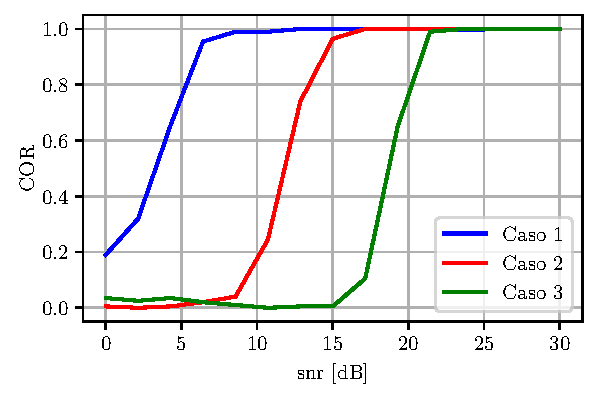
\includegraphics[width = 0.7\textwidth]{Figuras/COR_BIC_pruebas.pdf}
	\caption{COR para $BIC-lp$ en función de la SNR.}
	\label{fig:COR_example_bic}
\end{figure}

Los resultados se muestran en la figura \ref{fig:COR_example_bic}. Para el caso 1 se obtiene una buena estimación del orden a partir de 5dB. Sin embargo, para los casos 2 y 3 se ve que la performance de la estimación se ve degradada. Esto se debe a que al tener frecuencias muy cercas entre sí o con energía muy pequeña, no se obtienen buenas estimaciones de los modos, lo que lleva a una estimación errónea del Hessiano y repercute en la estimación del orden. 


\section{Selección del modelo explotando la estructura Hankel }\label{sec:review}
	 
	Debido al Teorema \ref{Th:Kronecker2} enunciado en el  capítulo \ref{chap:ModeloSumExp}, existe una relación entre el orden del modelo exponencial y el rango de su matriz de Hankel asociada. Además, este resultado se puede asociar con las aproximaciones de Padé o con la propiedad de invariancia de la matrices de Hankel. En está sección se explorará ambas alternativas para encontrar el orden del modelo.
	% 	Recordando el Teorema \ref{Th:Kronecker2}, el orden del modelo se puede estimar como el rango de la matriz de Hankel o también encontrando la aproximación de Padé, $R_{r-1,r}(z)$.

\subsection{Aproximaciones de Padé}

	De la sección \ref{sec:pade}, se puede asociar una aproximación de Padé $R_{r-1,r}(z)$ para el modelo exponencial definido en \eqref{Eq:Eq:NoiselessSignal}. En este camino, los autores en \cite{Gonnet2013} aproximan el símbolo asociado a la matriz de Hankel del modelo exponencial encontrando una aproximación de bajo orden. Considerando el caso especial de la aproximación de Padé $R_{n-1,n}$, de la relación \eqref{Eq:PadeApprox1} se obtiene el siguiente sistema de ecuaciones
	\begin{equation}
		\begin{bmatrix} a_n \\[0.3em] \vdots \\[0.3em] a_{2n-1} 
		\end{bmatrix} = \begin{bmatrix} x_n & x_{n-1} & \cdots & x_0 \\[0.3em] x_{n+1} & x_{n} & \cdots & x_1 \\[0.3em]
		\vdots & & \ddots & & \\[0.3em]
		x_{2n-1} & x_{2n-2} & \cdots & x_n
	\end{bmatrix}\begin{bmatrix} b_0 \\[0.3em] \vdots\\[0.3em] b_n \end{bmatrix}.
	\label{eq:ToeplitsSystem}
	\end{equation}
	Esta ecuación toma la forma de
	\begin{equation}
		\mathbf{0} = \matC\b,
		\label{eq:ToeplitsSystem2}
	\end{equation}
	donde el vector $\b$ contiene los coeficientes del polinomio del denominador $R_{n-1,n}$. El determinante de la matriz $\matC$ juega un papel crucial en la aproximación de Padé. Cuando este determinante es distinto de cero, se puede encontrar una aproximación de Padé para el sistema sin problemas. Si bien la matriz $\matC$ tiene estructura Toeplitz, se puede invertir fácilmente a una matriz con estructura Hankel. En \cite{Gonnet2013} utilizan la descomposición en valores singulares de $\matC\in\C^{n\times n+1}$,
	\begin{equation}
		\matC = \matU\Sigmab\matV^H,
	\end{equation} 
	donde $\Sigmab$ es una matriz diagonal, tal que sus elementos son los valores singulares $\sigma_1\ge\sigma_2\ge\cdots\ge\sigma_n$. Si $\sigma_n>0$, entonces $\rank(\matC) = n$ y la última columna de la matriz $\matV$ proporciona un vector no-nulo $\b$. Por otro lado, si $\sigma_{n} = 0$, $\rank(\matC) = \rho\le n$, con $\sigma_{\rho+1}=\cdots=\sigma_{n}=0$. En particular, la submatriz que contiene los últimos $\rho+1$ columnas de $\matC$ tiene rango deficiente, por lo que el espacio nulo de $\matC$ contiene un vector no nulo donde sus primeros $n-\rho$ elementos son cero. Por lo tanto, se puede hacer una reducción del grado de la aproximación de Padé a $R_{\rho-1,\rho}$ y volver al plantear el sistema \eqref{eq:ToeplitsSystem2} para orden $\rho$.
	
	Para el caso de señales ruidosas, el símbolo asociado a $\Hank_{\y}$ es
	\[\tilde{f}(z) = \sum_{k=1}^{\infty}(x_k+w_k)z^{-k}.\]
	La teoría de aproximación de Padé garantiza que la secuencia $\{R_{n-1,n}\}_{n\in\N}$ converge a $\tilde{f}(z)$ en probabilidad para un $n$ suficientemente grande. A medida que se aumenta el grado del polinomio del denominador por encima de $n$, aparecen pares espurios de polos y ceros en la aproximación de Padé. Para este caso, se puede pensar que la matriz $\matC$ en \eqref{eq:ToeplitsSystem2} estará perturbada por una matriz cuya norma espectral es al menos $\varepsilon$, entonces cada valor singular se ve perturbado como máximo por $\varepsilon$.  Por lo tanto, en \cite{Gonnet2013}, se propone realizar las mismas operaciones que para el caso no ruidoso, pero tratar un valor singular como cero si es menor que cierto umbral. Los autores proponen como umbral $\mathrm{tol}\cdot\|\x\|_2$, donde $\x=\big[x_0,\cdots,x_{2n-1}\big]$, y $\mathrm{tol}$ es una tolerancia relativa. Dado que el umbral estará definido por el usuario, la estimación del orden puede resultar incorrecta, dado que un umbral muy grande puede resultar en órdenes más chicos; y si umbrales pequeños resultar en órdenes más grandes. Esta observación se puede complementar dado el siguiente ejemplo. Se arman el modelo exponencial usando los parámetros dados en la la tabla \ref{Tab:vexpa_parameters_pade}. 	Además, se agrega ruido Gaussiano blanco circular a la señal y se normaliza el ruido para que tenga una norma infinita igual a $2\times 10^{-3}$.  
	
	\begin{table}[ht]
		\centering
		\begin{tabular}{l|llll}
			& \multicolumn{4}{l}{Ejemplo tomado de \cite{Cuyt2018}}  \\ \hline
			$\nu_i$        & 1.5  & 15.7   & 40   & 25.2    \\
			$\gamma_i$     & 0.0  & 0.0    & -0.0159 & -0.0477 \\ 
			$|a_i|$      & 0.001 & 2.0     & 4.0     & 8.0    \\
			$\angle a_i$ & 0.0    & 0.0    & 0.0    & 0.0    \\ \hline
		\end{tabular}
		\caption{Parámetro usados en la simulación numérica para el desempeño de \cite{Gonnet2013}.}
		\label{Tab:vexpa_parameters_pade}
	\end{table}

	Se realiza una estimación del orden usando el algoritmo en \cite{Gonnet2013} para diferentes realizaciones de ruido tomando dos tolerancias, $1\times 10^{-5}$ y $5\times 10^{-5}$. Para ello, se realizan simulaciones de Monte Carlo para diferentes escenarios haciendo 200 simulaciones para cada uno.
	
	\begin{figure}
		\centering
		\begin{subfigure}{0.45\linewidth}
			\centering
			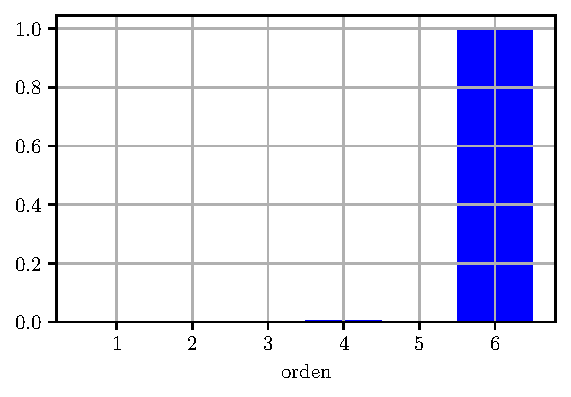
\includegraphics[width = \linewidth]{Figuras/orden_pade_svd_1e5.pdf}
			\caption{Ordenes estimados usando tolerancia \hspace*{1cm}$1\times10^{-5}$.}
			\label{fig:Hist_pade1}
		\end{subfigure}
		\begin{subfigure}{0.45\linewidth}
			\centering
			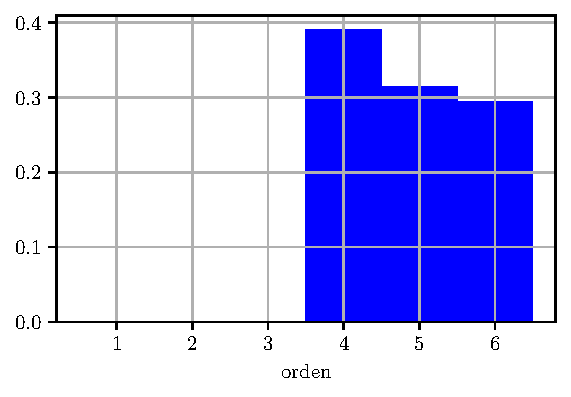
\includegraphics[width = \linewidth]{Figuras/orden_pade_svd_5e5.pdf}
			\caption{Ordenes estimados usando tolerancia \hspace*{1cm}$5\times10^{-5}$.}
			\label{fig:Hist_pade2}	
		\end{subfigure}
		\caption{Histogramas para el orden estimado usando el algoritmo \cite{Gonnet2013}}
		\label{fig:Hist_pade}
	\end{figure}

	En la figura \ref{fig:Hist_pade} se muestran los histogramas de los ordenes obtenidos en las realizaciones de Monte Carlo para las dos tolerancias propuestas. Cuando se usa como tolerancia $1\times 10^{-5}$ se puede observar en la figura \ref{fig:Hist_pade1} que el orden estimado siempre es mas grande que el real. Sin embargo, usando la tolerancia $5\times 10^{-5}$ en la figura \ref{fig:Hist_pade2} en algunas realizaciones se llega a estimar el orden correctamente.
	
	
	La aproximación de Padé se verá afectado por los $n-r$ combinaciones de polos y ceros no deseado que se suman a los $r$ polos y $r-1$ de la aproximación de $f(z)$, el polo y el cero en el par casi se cancelan entre sí localmente. En \cite{Cuyt2018} se observó que la inclusión de pares adicionales de polos y ceros en el modelo proporciona una representación más adecuada del ruido inherente al sistema. En consecuencia, se notó que se amplía la brecha para la determinación del número de valores singulares relevantes presentes en la matriz de Hankel asociada a la señal ruidosa. Este ajuste en la cantidad de valores singulares significativos se vuelve crucial a medida que la cantidad de muestras de la señal aumenta, lo que permite revelar con mayor precisión la estructura subyacente del sistema. No obstante, en situaciones prácticas, la obtención de una cantidad extensa de datos puede no ser factible. Este desafío se agrava en paralelo con el incremento de la potencia del ruido presente en la señal, ya que la distancia entre los valores singulares tiende a disminuir.
	
	Debido al teorema de convergencia de Padé \cite{NUTTALL1970}, los polos verdaderos pueden identificarse como polos estables en los sucesivas aproximaciones $\{R_{n-1,n}\}_{n\in\N}$, mientras que los polos ruidosos se distinguen por su inestabilidad. Al aumentar $n$ se obtiene un conjunto mayor de polos, de los cuales los ruidosos se mueven para cada realización diferente del ruido. Los verdaderos $z_i$ formaran grupos estables mientras los relacionados con el ruido estarán dispersos. Esta característica permite desarrollar un algoritmo de validado \cite{BRIANI2020} para la identificación de los parámetros desconocidos del modelo exponencial. Este algoritmo se basa en hacer un decimado por debajo de la frecuencia de Nyquist y utiliza técnicas de agrupamiento para distinguir los polos estables de aquellos que son espurios. A continuación se hará una breve descripción del algoritmo.
	 
	 
	
	
	%Por otro lado, cabe señalar que en \cite{Cuyt2018} se observó que la inclusión de pares adicionales de polos y ceros en el modelo proporciona una representación más adecuada del ruido inherente al sistema. En consecuencia, se notó que se amplía la brecha para la determinación del número de valores singulares relevantes presentes en la matriz de Hankel asociada a la señal ruidosa. Este ajuste en la cantidad de valores singulares significativos se vuelve crucial a medida que la cantidad de muestras de la señal aumenta, lo que permite revelar con mayor precisión la estructura subyacente del sistema. No obstante, en situaciones prácticas, la obtención de una cantidad extensa de datos puede no ser factible. Este desafío se agrava en paralelo con el incremento de la potencia del ruido presente en la señal, ya que la distancia entre los valores singulares tiende a disminuir.
	
	
	%Para superar esta situación, en \cite{BRIANI2020}  se propone un algoritmo conocido como VEXPA. Este algoritmo se basa en hacer un decimado por debajo de la frecuencia de Nyquist y utiliza técnicas de agrupamiento para distinguir los polos estables de aquellos que son espurios. Esta estrategia tiene un buen rendimiento de estimación en régimen de alta SNR. Desafortunadamente, el algoritmo requiere establecer varios parámetros que definen críticamente el rendimiento de estimación. A continuación se hará una breve descripción del algoritmo.
	
	\subsubsection{VEXPA (Validated EXPonential Analysis)}\label{VEXPA_Appendix}

	 Dado un factor de decimación $u$, se considera el modelo 
		\begin{equation}
			x_{ku} = \sum_{i=1}^r c_iz_i^{ku}, \quad k = 0,\ldots, 2r-1
			\label{eq:decimatedVEXPA}
		\end{equation}
		de manera que al plantear el problema de autovalores generalizados con las matrices de Hankel asociados a la señal \eqref{eq:decimatedVEXPA}, los autovalores obtenidos serán $z_i^u$, $i=1,\ldots, r$. Si estos autovalores se escriben como $z_i^u = e^{u\xi_iT_s}$, donde $\xi_i\in \C$ y $T_s$ un período de muestreo dado, la parte imaginaria de $\xi_i$ no puede recuperar de forma única, debido a que 
		\[|\Im(u\xi_iT_s)|<u\pi.\]
		De modo que puede aparecer el problema de \emph{aliasing}. Dada la periodicidad de la función $e^{\jmath u\Im(\xi_i)T_s}$ se puede identificar $u$ valores posibles de $\xi_i$ en el intervalo  $(-u\pi,u\pi)$.

		El problema de \emph{aliasing} puede resolverse agregando $r$ muestras a la señal decimada \\ $x_0,x_u,\ldots,x_{(2r-1)u}$, en los puntos desplazados $kuT_s + s T_s$ para $k = h,\ldots,h+r-1$ con $0\le h\le r$. Los números $u$ y $s$ deben ser números mutuamente primos.
	
		De las muestras $x_0,x_u,\ldots,x_{(2r-1)u}$ se obtienen autovalores generalizados $z_i^u$ y coeficientes $c_i$ a partir del sistema lineal \eqref{eq:decimatedVEXPA}. De modo que se obtienen los coeficientes $c_i$ correspondiente a cada $z_i^u$, pero aun no se puede identificar $\Im(\xi_i)$ correcto a partir de $z_i^u$. Sin embargo, las muestras adicionales que se agregan cumplen que 
		\[x_{ku + s} = \sum_{i=1}^r (c_iz_i^{s})z_i^{uk}, \quad k = h,\ldots, h+r-1. \]
		De este sistema se pueden obtener $c_1z_1^{s}, \ldots,c_rz_r^{s}$ asociados a $z_i^u$. Es decir, se obtiene un conjunto de $s$ valores posibles para $\xi_i$ en el intervalo  $(-s\pi,s\pi)$. Debido a que $s$ y $u$ son números mutuamente primos, los dos conjuntos de posibles para $\xi_i$ tienen solo un valor en su intersección. 

		De modo que los autovalores generalizados asociados a la señal $x_k$ se agrupan cerca del valor real de $z_i^u$, y similarmente para $z_i^{s}$, mientras que otros autovalores se asocian a realizaciones de ruido y no suelen estar agrupados.  
		
		Para encontrar estos cluster de autovalores, VEXPA usa el algoritmo DBSCAN \cite{ester1996}. DBSCAN es una algoritmo de agrupamiento no paramétrico basado en densidad, es decir, dado un conjunto de untos en algún espacio, agrupa puntos que están muy juntos (puntos con muchos vecinos cercanos), marcando como valores atípicos los puntos que se encuentran solos en regiones de baja densidad (cuyos vecinos más cercanos están demasiado lejos). A diferencia de algoritmos de agrupación tradicionales como K-means, DBSCAN no requiere especificar el número de grupos de antemano, lo que lo hace adecuado para situaciones en las que no se conoce el número de grupos. Sin embrago, puede ser sensible a la elección de parámetros y puede tener dificultades con grupos de densidad variable. 
		
		
		Esta estrategia tiene un buen rendimiento de estimación en régimen de alta SNR. Desafortunadamente, VEXPA  requiere establecer varios parámetros que definen críticamente el rendimiento de estimación. 
		
		Dado el modelo exponencial definido en \eqref{Eq:Eq:NoiselessSignal}, utilizando los parámetros dados en la tabla \ref{tab:vexpa_parameters}, se realiza una comparación cualitativa para diferentes regímenes de SNR y diferentes parámetros del algoritmo VEXPA. Para ello, se realizan simulaciones de Monte Carlo para diferentes escenarios haciendo 200 simulaciones para cada uno. Para realizar el análisis se calcula la tasa de estimación correcta del orden correcto (COR), es decir, 
		\[\mathrm{COR} = \frac{\text{número de veces } \hat{r}=r}{M}.\]
		  
		\begin{table}[ht]
			\centering
			\begin{tabular}{l|llllllllllll}
					& \multicolumn{12}{l}{Ejemplo tomado de \cite{BRIANI2020}}  \\ \hline
				$\nu_i$      & -5.93  & -4.05   & -3.10   & -1.82  & -1.31        & 1.90   & 2.97    & 6.05    & 6.67   & 
				38.0         & 43.0   & -24.0 \\
				$\gamma_i$   & 0.0    & 0.0     & 0.0     & 0.0    & 0.0          & 0.0    & 0.0     & 0.0     & 0.0    & 
				0.0          & 0.0    & 0.0 \\
				$|a_i|$      & 1.0    & 2.0     & 2.0     & 2.0    & 2.0          & 1.0    & 3.0     & 1.5     & 2.0    &
				3.0          & 1.0    & 1.0    \\
				$\angle a_i$ & 0.0    & 3.14    & 0.78    & 0.39   &
				2.35         & 0.31   & -3.14   & -2.74   & 0.0    &
				-2.45        & 0.0    & 0.628        \\ \hline
			\end{tabular}
			\caption{Parámetro usados en la simulación numérica para el desempeño de VEXPA.}
			\label{Tab:vexpa_parameters}
		\end{table}
	
		En principio se observa que para ejecutar VEXPA con DBSCAN se necesitan elegir cinco parámetros diferentes. Se ejecutó el algoritmo de estimación de orden usando diferentes combinación de estos parámetros. Al comparar su desempeño, en la figura \ref{fig:COR_example_vexpa} se observa que el algoritmo es muy sensible a la elección de los parámetros. Se observa que VEXPA no obtiene una buen rendimiento para SNR por de bajo de 5dB, y para algunos parámetros esta observación se extiende por debajo de los 10dB. 
		
		\begin{figure}[ht]
			\centering
			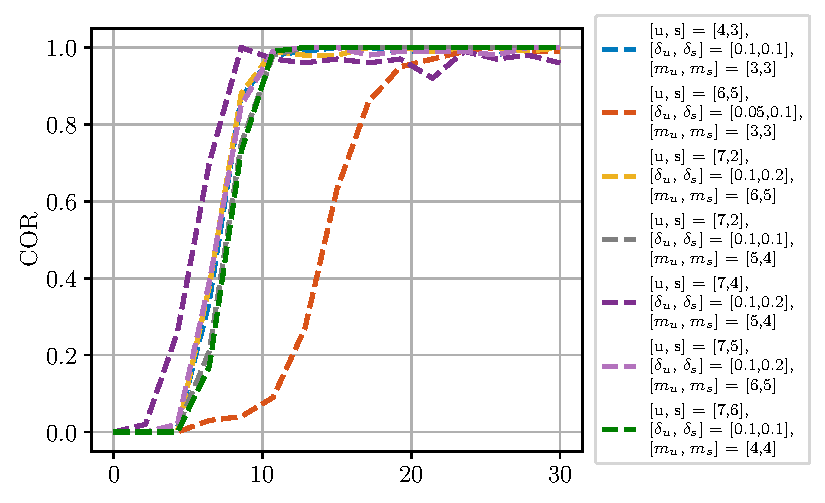
\includegraphics[width = 0.7\textwidth]{Figuras/vexpa_example.pdf}
			\caption{COR para VEXPA en función de la SNR.}
			\label{fig:COR_example_vexpa}
		\end{figure}
		
		Por otro lado, otro problema que se observa en \cite{BRIANI2020} es que cuando los modos oscilatorios se agrupan muy cerca entre sí se necesita utilizar múltiples ejecuciones de DBSCAN para obtener un buen rendimiento, traduciéndose en más tiempo de procesamiento para obtener la estimación del orden del modelo.
			
\subsection{Principio de invariancia}	

Los métodos de estimación espectral como el MPM o ESPRIT explotan el principio de invariancia, dada la relación obtenida en \eqref{Esprit:eq}.  La distancia entre el subespacio generado por las columnas de $\matU_{f}$  y del generado por las columnas $\matU_l$ resulta clave para estimar el orden del modelo. Como medida de proximidad, se usaran los ángulos principales entre estos dos subespacios. A continuación se reproducen tanto la definición de ángulos principales y resultados relacionados, para luego estudiar como estos ángulos se puede estimar el orden del modelo.
\subsubsection{Lemas y definiciones auxiliares}

 Para demostrar los resultados obtenidos en esta sección serán útiles los siguientes resultados y definiciones 

\begin{definition}[\cite{Stewart1990}]\label{def:principalAngles}
	Sean $\setX$, $\setY$ dos subespacios con $\dim(\setX) = \dim(\setY)=s$. Los ángulos principales entre $\setX$ y $\setY$ son
	\begin{equation*}
		\Thetab(\setX,\setY) = \big[\theta_1, \ldots, \theta_s\big],\quad \theta_k\in[0,\pi/2],\quad k=1,\ldots,s
	\end{equation*}
	definidos por
	\begin{equation}
		\cos\theta_k = \max_{\stackrel{\x\in\setX}{\y\in\setY}}\bigg\{\frac{|\langle\x,\y\rangle|}{\|\x\|_2\|\y\|_2} : \x^H\x_i = 0,\ \y^H\y_i = 0,  \forall i\in\{1,\ldots,k-1\}\bigg\}.
		\label{Eq:principalAngles2}
	\end{equation}
\end{definition}

\begin{lemma}\label{Lemma:Angulos}
		$\setX = \setY$ si y solo si $\Thetab(\setX,\setY) = \mathbf{0}$
	\end{lemma}
	\begin{proof}
		Por construcción, los vectores $\{\x_1,\ldots,\x_s\}$ forman un base del subespacio $\setX$. De igual forma $\{\y_1,\ldots,\y_s\}$ es una base $\setY$. Si $\cos\theta_k=1$, se tiene que $\x_k$ e $\y_k$ están alineados. Por lo tanto, si todos los ángulos principales son cero, los conjuntos  $\{\x_1,\ldots,\x_s\}$ y $\{\y_1,\ldots,\y_s\}$ generan el mismo subespacio.
		
		Por otro lado, cuando $\setX=\setY$, es claro que 
		\[\max_{\stackrel{\x\in\setX}{\y\in\setY}}\frac{|\langle\x,\y\rangle|}{\|\x\|_2\|\y\|_2} = 1\]
		y por lo tanto, $\cos\theta_k = 1$ para todo $k$.
	\end{proof}
	
	\begin{definition}
		La distancia entre los subespacios $\setX$ e $\setY$ está dada por
		\begin{equation}
			\rho(\setX,\setY) = \max\bigg\{\max_{\stackrel{\x\in\setX}{\|\x\|_2=1}}\dist(\x,\setY),\max_{\stackrel{\y\in\setY}{\|\y\|_2=1}}\dist(\y,\setX) \bigg\}
			\label{Eq:GapDistance}
		\end{equation}
	\end{definition}
	
	\begin{prop}\label{Prop:GapDistance}
		Sean $\setX$ e $\setY$ dos subespacio, se definen $\matProj_{\setX}$ y $\matProj_{\setY}$ la proyección ortogonal sobre $\setX$ e $\setY$ respectivamente. Luego,
		\begin{itemize}
			\item[i)] $\rho(\setX,\setY)=\sin\theta_1$, con $\theta_1$ es el máximo ángulo principal entre $\setX$ e $\setY$.
			\item[ii)] $\rho(\setX,\setY) = \|\matProj_{\setX}-\matProj_{\setY}\|_2$.
		\end{itemize} 
	\end{prop}
	\begin{proof}
        Sean  $\matX\in\C^{n\times s}$ e $\matY\in\C^{n\times s}$ matrices cuyas columnas forman una base orthonormal para los subespacios $\setX$ e $\setY$ respectivamente. Por lo tanto, se definen las matrices de proyección $\matProj_{\setX} = \matX\matX^H$ y $\matProj_{\setY} = \matY\matY^H$.
        
        Como consecuencia de la descomposición coseno-seno \cite{Stewart1990} existen matrices unitarias $\matU,\matV\in\C^{s\times s}$ y $\matQ\in\C^{n\times n}$ tal que si $2s\le n$,
            \[\matQ\matX\matU = \begin{bmatrix} \matI_s\\[0.3em] \mathbf{0}\\[0.3em]\mathbf{0}\end{bmatrix},\qquad \matQ\matY\matV = \begin{bmatrix}\matC\\[0.3em] \matS\\[0.3em] \mathbf{0}\end{bmatrix}\]
            donde $\matC, \matS$ son matrices diagonales tal que \[\matC = \diag(\cos\theta_1,\cdots,\cos\theta_s), \qquad \matS = \diag(\sin\theta_1,\cdots,\sin\theta_s).\] Además cumplen que $\matC^2+\matS^2=\matI$. Luego,

            \[\begin{aligned} \matQ\matProj_{\setX}(\matI-\matProj_{\setY})\matQ & = \begin{bmatrix} \matI & \mathbf{0} & \mathbf{0}\\[0.3em] \mathbf{0} & \mathbf{0} & \mathbf{0}\\[0.3em] \mathbf{0} & \mathbf{0} & \mathbf{0}
            \end{bmatrix}\begin{bmatrix} \matI - \matC^2 & -\matC\matS & \mathbf{0}\\[0.3em] -\matS\matC & \matS^2 & \mathbf{0}\\[0.3em] \mathbf{0} & \mathbf{0} & \mathbf{0}
            \end{bmatrix}\\[0.3em]
            & = \begin{bmatrix} \matI - \matC^2 & -\matC\matS & \mathbf{0}\\[0.3em] \mathbf{0} & \mathbf{0} & \mathbf{0}\\[0.3em] \mathbf{0} & \mathbf{0} & \mathbf{0}
            \end{bmatrix} = \begin{bmatrix} \matS^2 & -\matC\matS & \mathbf{0}\\[0.3em] \mathbf{0} & \mathbf{0} & \mathbf{0}\\[0.3em] \mathbf{0} & \mathbf{0} & \mathbf{0}
            \end{bmatrix}\\[0.3em]
            & = \begin{bmatrix}\matS\\[0.3em]\mathbf{0}\\[0.3em] \mathbf{0}\end{bmatrix}\begin{bmatrix} \matS & -\matC & \mathbf{0} 
            \end{bmatrix}. \end{aligned}\]

            Dado que las filas de $\begin{bmatrix} \matS & -\matC & \mathbf{0} 
            \end{bmatrix}$ son ortonormales, los valores singulares de $\matQ\matProj_{\setX}(\matI-\matProj_{\setY})\matQ$ son $\sin\theta_1,\sin\theta_2,\sin\theta_3,\ldots$. Por lo tanto,
            
            \begin{equation}\|\matProj_{\setX}(\matI-\matProj_{\setY})\|_2 = \sin\theta_1.\label{Eq:appendix_sin1}\end{equation}

            De una forma similar, se obtiene
             \[\matQ(\matProj_{\setX} - \matProj_{\setY})\matQ  =  \begin{bmatrix} \matS^2 & -\matC\matS & \mathbf{0}\\[0.3em] -\matC\matS & -\matS^2 & \mathbf{0}\\[0.3em] \mathbf{0} & \mathbf{0} & \mathbf{0}
            \end{bmatrix}.\]
             Dado que $\matS$ y $\matC$ son matrices diagonales, los valores singulares de $\matProj_{\setX}-\matProj_{\setY}$ son los valores singulares de las matrices de $2\times 2$
            \[\begin{bmatrix} \sin\theta_i & -\cos\theta_i\sin\theta_i\\[0.3em] -\sin\theta_i\cos\theta_i & -\sin\theta_i\end{bmatrix}, \quad i = 1,\ldots, s,\]
            que son $\sin\theta_i$ dos veces. Por lo tanto, como la norma espectral es igual al máximo valor singular, se obtiene
            \begin{equation} \|\matProj_{\setX} - \matProj_{\setY}\|_2 = \sin\theta_1.\label{Eq:appendix_sin2}\end{equation}

            
		\begin{itemize}
		    \item[i)] La distancia entre un vector y un subespacio se puede escribir como
                    \[dist(\x,\setY) = \|(\matI -\matProj_{\setY})\x\|_2.\]
                    Luego,
                    \[\begin{aligned} \max_{\stackrel{\x\in\setX}{\|\x\|_2=1}} \|(\matI -\matProj_{\setY})\x\|_2 & = \max_{\stackrel{\x\in\setX}{\|\x\|_2\le }} \|(\matI -\matProj_{\setY})\x\|_2\\[0.3em]
                    & = \max_{\|\x\|_2=1}\|(\matI-\matProj_{\setY})\matProj_{\setX}\x\|_2 \\[0.3em]
                    & = \|(\matI-\matProj_{\setY})\matProj_{\setX}\|_2 = \sin\theta_1.
                    \end{aligned}\]
                    Donde la última igual se obtiene de \eqref{Eq:appendix_sin1}
                    De la misma forma, se obtiene que 
                    \[\max_{\stackrel{\y\in\setY}{\|\y\|_2=1}}\dist(\y,\setX) = \|(\matI-\matProj_{\setX})\matProj_{\setY}\|_2 = \sin\theta_1.\]
                Por lo tanto, se obtiene que 
                \[\rho(\setX,\setY) = \sin\theta_1.\]
                
            \item[ii)] Como se observo en \eqref{Eq:appendix_sin2} el máximo valor singular de $\matProj_{\setX}-\matProj_{\setY}$ es $\sin\theta_1$. Por lo tanto se obtiene
            \[\rho(\setX,\setY) = \|\matProj_{\setX}-\matProj_{\setY}\|_2\]
            
		\end{itemize}
	\end{proof}
	

\subsubsection{Estructura algebraica de la señal}

    Al considerar el caso sin ruido, usando la descomposición en valores singulares \eqref{Eq:SVD} asociada al modelo exponencial, se define $\matU(s) = \big[\u_1,\ldots,\u_s\big]$ como la matriz que contiene los primeros $s$ vectores singulares $\u_i$. Como se demostró en el Capítulo \ref{chap:ModeloSumExp}, las columnas de la matriz $\matU(r)$ generan el subespacio de señal. Este subespacio tiene dimensión $r$, que a su vez es igual al orden del modelo. Definiendo las siguiente matrices
\begin{equation}
	\begin{aligned} 
		& \matU_f(s) = \begin{bmatrix} \mathbf{0}_{(n-1)\times 1} & \matI_{n-1}\end{bmatrix}\matU(s), \quad
		\matU_l(s) = \begin{bmatrix}  \matI_{n-1} & \mathbf{0}_{(n-1)\times 1} \end{bmatrix}\matU(s).
	\end{aligned}
	\label{Eq:matrices_lf}
\end{equation}
Usando \eqref{Eq:Invariance}, se construye el siguiente haz matricial
\begin{equation}
	\matU_f(r) = \matU_l(r)\boldsymbol{\Phi},
	\label{Um:eq}
\end{equation}
donde  $\Phib \in \C^{r \times r}$ es una matriz nosingular. A continuación, considerando

\begin{equation}
	\matE(s) = \matU_f(s) - \matU_l(s)\matU_l(s)^\dagger\matU_f(s).
	\label{eq:rhatESTER}
\end{equation}
Claramente, cuando $s=r$, $\matE(s)= \mathbf{0}$.

Los autores en \cite{Badeau2006} proponen el método ESTimation Error Rule (ESTER) para estimar $r$ mediante la minimización del función $\matE(s)$, es decir,
\begin{equation}
	\hat{r}_{\mathrm{ESTER}} = \arg\min_s\|\matE(s)\|_2.
	\label{Eq:ESTER_Rule}
\end{equation}

Una propuesta alternativa es propuesta en \cite{Papy2007}, donde los autores consideran la matriz aumentada de $n\times 2s$
\[ \matE_{aug}(s) = \big[\matU_f(s)\ \matU_l(s)\big].\]
Sea $\gamma_1\ge\cdots\gamma_{2s}$ los valores singulares de $\matE_{aug}(s)$. Cuando $s\ge r$, $\gamma_{r+1} = \cdots =\gamma_{2s} = 0$. La técnica SAMOS (Subspace based Automatic Model Order Selection) estima el orden del modelo $r$ como la solución del siguiente problema de optimización
\begin{equation}
	\hat{r}_{\mathrm{SAMOS}} = \arg\min_s\frac{1}{s}\sum_{i=s+1}^{2s} \gamma_i. 
	\label{eq:rhatSAMOS}
\end{equation}

De acuerdo a \eqref{Um:eq} $\matU_l(r)$ y $\matU_f(r)$ generan el mismo subespacio. Por lo tanto, la distancia entre los espacios columna de estas dos matrices proporciona un elemento clave para poder estimar $r$. Como medida para medir la proximidad entre dos subespacio se utilizarán los ángulos definidos en \eqref{def:principalAngles}. Teniendo en cuenta la proposición \eqref{Prop:GapDistance}, se formulan los siguientes resultados.

\begin{theorem}\label{The1:ESTER_GAP}
	Sea $\theta_1(s),\ge\cdots\ge\theta_s(s)$ los ángulos principales entre los subespacios generados por los vectores columnas de $\matU_f(s)$ y $\matU_l(s)$. Luego,
	\begin{equation}
		\|\matE(s)\|_2  \le \sin\theta_1(s)
		\label{Eq:ESTERBound}
	\end{equation}
\end{theorem}  
\begin{proof} Considerando la descomposición polar de $\matU_f(s)$ y $\matU_l(s)$
	\begin{equation}
		\begin{aligned}
			& \matU_f(s) = \hat{\matU}_f(s)\big(\matI_s -         \u_f^H\u_f\big)^{\frac{1}{2}}\\
			& \matU_l(s) = \hat{\matU}_l(s)\big(\matI_s -         \u_l^H\u_l\big)^{\frac{1}{2}}
		\end{aligned}
		\label{Eq:nearest_Orthonormal}
	\end{equation}
	donde $\u_f\in\C^{1\times s}$ ($\u_l\in\C^{1\times s}$) es la primera (última) fila de $\matU(s)$, y $\hat{\matU}_f(s)$ y $\hat{\matU}_l(s) $ son matrices de $(m-1)\times s$, ambas con columnas ortonormales. Las proyecciones ortogonales sobre los espacio columna de  $\matU_f(s)$ y $\matU_l(s)$ son:  
	\begin{equation}
		\begin{aligned}
			& \matProj_f(s) = \matU_f(s)\matU_f(s)^\dagger = \hat{\matU}_{f}(s)\hat{\matU}_{f}^H(s) \\
			& \matProj_l(s) = \matU_l(s)\matU_l(s)^\dagger = \hat{\matU}_{l}(s)\hat{\matU}_{l}^H(s),
		\end{aligned}
		\label{Eq:ProjMatrix}
	\end{equation}
	donde $\matU_l(s)^\dagger$ es la pseudo-inversa de Moore-Penrose. 
	Dado que $\hat{\matU}_f$ y $\hat{\matU}_l$ tienen columnas ortonormales, sea
	\[\begin{aligned} \|\hat{\matE}(s)\|_2 & = \|\hat{\matU}_{f}(s) -\hat{\matU}_{l}(s)\hat{\matU}_l^H(s)\hat{\matU}_f(s)\|_2 \\\ & = \|\left(\hat{\matU}_{f}(s)\hat{\matU}_{f}^H(s) -\hat{\matU}_{l}(s)\hat{\matU}_l^H(s)\right)\hat{\matU}_f(s)\|_2\\
		&  = \|\matProj_f(s) - \matProj_l(s)\|_2 = \sin \theta_1(s)
	\end{aligned}
	\]
	donde en la última igualdad se uso la Proposición \ref{Prop:GapDistance}. Luego,
	\begin{equation}
		\begin{aligned} \|\matE(s)\|_2 & = \|\matU_{f}(s) -\matU_{l}(s)\matU_l(s)^\dagger\matU_f(s)\|_2 \\
			&\le \|\matProj_f(s) - \matProj_l(s)\|_2\|\matU_f(s)\|_2 = \|\matU_f(s)\|_2\sin \theta_1(s). \end{aligned}
		\label{Eq:ESTER_gap_Theo}
	\end{equation}
	Dado que $\matU_f(s)$ es una submatriz de la matriz unitaria $\matU$, sus valores singulares serán como máximo iguales a 1. Por lo tanto,  usando $\|\matU_f(s)\|_2\leq 1$ se obtiene \eqref{Eq:ESTERBound} . \end{proof}


\begin{theorem}\label{The1:SAMOS}
	Sea $\gamma_1\ge\cdots\ge\gamma_{2s}$ los valores singulares de $\matE_{aug}(s)$. Luego,
	\begin{equation}
		\frac{1}{s}\sum_{i=s+1}^{2s}\gamma_i\le \sqrt{2}\left[1+\frac{1}{s}\sum_{i=1}^s\sin\frac{\theta_{i}(s)}{2}\right].
		\label{eq:Angle_Weyl}
	\end{equation}
\end{theorem}
\begin{proof}
	Recordando que $\matU_f(s)$ es una matriz de rango completo, las matrices $\matU_f(s)$ y $\hat{\matU}_f(s)$ generan el mismo espacio columna, lo mismo vale para $\matU_l(s)$ y $\hat{\matU}_l(s)$, con $\hat{\matU}_f(s)$ y $\hat{\matU}_l(s)$ definidos en \eqref{Eq:nearest_Orthonormal}. Luego, los ángulos principales entre $\matU_f(s)$ y $\matU_l(s)$ son los mismo que los ángulos entre $\hat{\matU}_f(s)$ y $\hat{\matU}_l(s)$. Definiendo
	\begin{equation}
		\hat{\matE}_{aug}(s) = \begin{bmatrix} \hat{\matU}_f(s) & \hat{\matU}_l(s)\end{bmatrix},
	\end{equation}
	notar que sus valores singulares se pueden obtener a partir de la matriz $\matI_{2s}+\matM$, donde
	\[\matM = \begin{bmatrix} \mathbf{0} & \hat{\matU}_f(s)^H\hat{\matU}_l(s)\\[0.3em] \hat{\matU}_l(s)^H\hat{\matU}_f(s) & \mathbf{0}
	\end{bmatrix}.\]
	De acuerdo con \cite[Teorema I.5.2]{Stewart1990}, los valores singulares de $\hat{\matU}_f(s)^H\hat{\matU}_l(s)$ ordenados en forma creciente son $\cos\theta_1(s),\ldots,\cos\theta_s(s)$. Luego, a partir de \cite[Teorema 7.3.3]{Horn1990}, los últimos $s$ valores singulares de $\hat{\matE}_{aug}$ ordenados en forma decreciente son
	\[\sqrt{1-\cos\theta_{i-s}(s)} = \sqrt{2}\sin\frac{\theta_{i-s}(s)}{2}\quad i= s+1,\ldots,2s.\]
	
	Sea $\matA = \matU_f(s) - \hat{\matU}_f(s)$ y $\matB = \matU_l(s) - \hat{\matU}_l(s)$, entonces, $\matE_{aug}(s) - \hat{\matE}_{aug}(s) = \left[ \matA\  \matB\right]$. Se puede demostrar que $\hat{\matU}_f(s)$ es la matriz con columnas ortonormales más cercana a  $\matU_f(s)$ \cite{Higham89}. La misma conclusión se obtiene entre $\hat{\matU}_l(s)$ y $\matU_l(s)$. Además,
	\[\|\matA\|_2 = \max_{i}|\zeta_i-1|,\]
	donde $\zeta_i$ es el $i-$ésimo valor singular de $\matU_f(s)$. Debido a que $\matU_f(s)$ es una submatriz de la matriz unitaria $\matU$ se tiene que  $\zeta_i\le 1$. Por lo tanto, $\|\matA\|_2\le 1$, y de forma similar se deduce que $\|\matB\|_2\le 1$. Luego, por el teorema de Weyl \cite[Teorema 4.11]{Horn1990}, los últimos $s$ valores singulares de $\matE_{aug}(s)$ y $\hat{\matE}_{aug}(s)$ está separados como mucho por $\|\left[ \matA\  \matB\right]\|_2$, es decir, para $i = s+1,\ldots, 2s$,
	\begin{equation}
		|\gamma_i -\sqrt{2}\sin\frac{\theta_{i-s}}{2}|\le \|\left[\matA\ \matB\right]\|_2\le \sqrt{\|\matA\|_2^2+\|\matB\|_2^2}\le \sqrt{2}.
	\end{equation}
	
	Usando la desigualdad triangular se obtiene
	\[\frac{1}{s}\sum_{i=s+1}^{2s}\gamma_i - \frac{1}{2}\sum_{i=s+1}^{2s}\sqrt{2}\sin\frac{\theta_{2s-i+1}(s)}{2} \le \frac{1}{2}\sum_{i=s+1}^{2s}\bigg|\gamma_i - \sqrt{2}\sin\frac{\theta_{2s-i+1}(s)}{2}\bigg|\le \sqrt{2}.\]
	
	Finalmente, 
	\[\frac{1}{s}\sum_{i=s+1}^{2s}\gamma_i\le\sqrt{2}+\frac{1}{s}\sum_{i=1}^s\sqrt{2}\sin\frac{\theta_i(s)}{2}\]
\end{proof}

A continuación se mostrará de forma experimental que los teoremas \ref{The1:ESTER_GAP} y \ref{The1:SAMOS} proveen cotas superiores ajustadas. Para ello, se simula una suma de $r$ exponenciales complejas, tomando diferentes valores de $r$. Para cada señal, las frecuencias $z_i=e^{2\pi\jmath f_i}$, se eligen tomando $r$ valores distribuidos uniformemente sobre el intervalo $(0,1]$. Las amplitudes complejas, $c_i$, son tomadas a partir de muestras de una distribución uniforme entre $[1, 1.5]$. La Figura \ref{Fig:BoundsAngles} muestra los resultados en función del parámetro $s$. Para evaluar la cota en el Teorema \eqref{The1:ESTER_GAP}, la figura \ref{Fig:ESTER_angles} muestra \[\big|\|\matE(s)\|_2 - \rho\big|.\] 
La cota del Teorema \eqref{The1:SAMOS} se analiza en la figura \ref{Fig:SAMOS_angles} donde se muestra \[1/s\big|\sum_i(\gamma_{s+i}-\sqrt{2}\sin(\theta_i/2))\big|.\]
Ambas figuras muestran que las cotas son ajustadas para todo $s$. Además, ambas alcanzan un mínimo cuando $s=r$.

\begin{figure}[t]
	\centering
	\begin{subfigure}{0.45\textwidth}
		\centering
		\resizebox{\linewidth}{!}{%% Creator: Matplotlib, PGF backend
%%
%% To include the figure in your LaTeX document, write
%%   \input{<filename>.pgf}
%%
%% Make sure the required packages are loaded in your preamble
%%   \usepackage{pgf}
%%
%% and, on pdftex
%%   \usepackage[utf8]{inputenc}\DeclareUnicodeCharacter{2212}{-}
%%
%% or, on luatex and xetex
%%   \usepackage{unicode-math}
%%
%% Figures using additional raster images can only be included by \input if
%% they are in the same directory as the main LaTeX file. For loading figures
%% from other directories you can use the `import` package
%%   \usepackage{import}
%%
%% and then include the figures with
%%   \import{<path to file>}{<filename>.pgf}
%%
%% Matplotlib used the following preamble
%%   \usepackage[utf8x]{inputenc}
%%   \usepackage[T1]{fontenc}
%%   \usepackage{amsmath,amssymb,amsfonts}
%%
\begingroup%
\makeatletter%
\begin{pgfpicture}%
\pgfpathrectangle{\pgfpointorigin}{\pgfqpoint{4.613765in}{2.790349in}}%
\pgfusepath{use as bounding box, clip}%
\begin{pgfscope}%
\pgfsetbuttcap%
\pgfsetmiterjoin%
\definecolor{currentfill}{rgb}{1.000000,1.000000,1.000000}%
\pgfsetfillcolor{currentfill}%
\pgfsetlinewidth{0.000000pt}%
\definecolor{currentstroke}{rgb}{1.000000,1.000000,1.000000}%
\pgfsetstrokecolor{currentstroke}%
\pgfsetdash{}{0pt}%
\pgfpathmoveto{\pgfqpoint{0.000000in}{0.000000in}}%
\pgfpathlineto{\pgfqpoint{4.613765in}{0.000000in}}%
\pgfpathlineto{\pgfqpoint{4.613765in}{2.790349in}}%
\pgfpathlineto{\pgfqpoint{0.000000in}{2.790349in}}%
\pgfpathclose%
\pgfusepath{fill}%
\end{pgfscope}%
\begin{pgfscope}%
\pgfsetbuttcap%
\pgfsetmiterjoin%
\definecolor{currentfill}{rgb}{1.000000,1.000000,1.000000}%
\pgfsetfillcolor{currentfill}%
\pgfsetlinewidth{0.000000pt}%
\definecolor{currentstroke}{rgb}{0.000000,0.000000,0.000000}%
\pgfsetstrokecolor{currentstroke}%
\pgfsetstrokeopacity{0.000000}%
\pgfsetdash{}{0pt}%
\pgfpathmoveto{\pgfqpoint{0.577239in}{0.547150in}}%
\pgfpathlineto{\pgfqpoint{4.513765in}{0.547150in}}%
\pgfpathlineto{\pgfqpoint{4.513765in}{2.690349in}}%
\pgfpathlineto{\pgfqpoint{0.577239in}{2.690349in}}%
\pgfpathclose%
\pgfusepath{fill}%
\end{pgfscope}%
\begin{pgfscope}%
\pgfpathrectangle{\pgfqpoint{0.577239in}{0.547150in}}{\pgfqpoint{3.936526in}{2.143199in}}%
\pgfusepath{clip}%
\pgfsetrectcap%
\pgfsetroundjoin%
\pgfsetlinewidth{0.803000pt}%
\definecolor{currentstroke}{rgb}{0.690196,0.690196,0.690196}%
\pgfsetstrokecolor{currentstroke}%
\pgfsetdash{}{0pt}%
\pgfpathmoveto{\pgfqpoint{0.644339in}{0.547150in}}%
\pgfpathlineto{\pgfqpoint{0.644339in}{2.690349in}}%
\pgfusepath{stroke}%
\end{pgfscope}%
\begin{pgfscope}%
\pgfsetbuttcap%
\pgfsetroundjoin%
\definecolor{currentfill}{rgb}{0.000000,0.000000,0.000000}%
\pgfsetfillcolor{currentfill}%
\pgfsetlinewidth{0.803000pt}%
\definecolor{currentstroke}{rgb}{0.000000,0.000000,0.000000}%
\pgfsetstrokecolor{currentstroke}%
\pgfsetdash{}{0pt}%
\pgfsys@defobject{currentmarker}{\pgfqpoint{0.000000in}{-0.048611in}}{\pgfqpoint{0.000000in}{0.000000in}}{%
\pgfpathmoveto{\pgfqpoint{0.000000in}{0.000000in}}%
\pgfpathlineto{\pgfqpoint{0.000000in}{-0.048611in}}%
\pgfusepath{stroke,fill}%
}%
\begin{pgfscope}%
\pgfsys@transformshift{0.644339in}{0.547150in}%
\pgfsys@useobject{currentmarker}{}%
\end{pgfscope}%
\end{pgfscope}%
\begin{pgfscope}%
\definecolor{textcolor}{rgb}{0.000000,0.000000,0.000000}%
\pgfsetstrokecolor{textcolor}%
\pgfsetfillcolor{textcolor}%
\pgftext[x=0.644339in,y=0.449928in,,top]{\color{textcolor}\rmfamily\fontsize{12.000000}{14.400000}\selectfont \(\displaystyle {0}\)}%
\end{pgfscope}%
\begin{pgfscope}%
\pgfpathrectangle{\pgfqpoint{0.577239in}{0.547150in}}{\pgfqpoint{3.936526in}{2.143199in}}%
\pgfusepath{clip}%
\pgfsetrectcap%
\pgfsetroundjoin%
\pgfsetlinewidth{0.803000pt}%
\definecolor{currentstroke}{rgb}{0.690196,0.690196,0.690196}%
\pgfsetstrokecolor{currentstroke}%
\pgfsetdash{}{0pt}%
\pgfpathmoveto{\pgfqpoint{1.091671in}{0.547150in}}%
\pgfpathlineto{\pgfqpoint{1.091671in}{2.690349in}}%
\pgfusepath{stroke}%
\end{pgfscope}%
\begin{pgfscope}%
\pgfsetbuttcap%
\pgfsetroundjoin%
\definecolor{currentfill}{rgb}{0.000000,0.000000,0.000000}%
\pgfsetfillcolor{currentfill}%
\pgfsetlinewidth{0.803000pt}%
\definecolor{currentstroke}{rgb}{0.000000,0.000000,0.000000}%
\pgfsetstrokecolor{currentstroke}%
\pgfsetdash{}{0pt}%
\pgfsys@defobject{currentmarker}{\pgfqpoint{0.000000in}{-0.048611in}}{\pgfqpoint{0.000000in}{0.000000in}}{%
\pgfpathmoveto{\pgfqpoint{0.000000in}{0.000000in}}%
\pgfpathlineto{\pgfqpoint{0.000000in}{-0.048611in}}%
\pgfusepath{stroke,fill}%
}%
\begin{pgfscope}%
\pgfsys@transformshift{1.091671in}{0.547150in}%
\pgfsys@useobject{currentmarker}{}%
\end{pgfscope}%
\end{pgfscope}%
\begin{pgfscope}%
\definecolor{textcolor}{rgb}{0.000000,0.000000,0.000000}%
\pgfsetstrokecolor{textcolor}%
\pgfsetfillcolor{textcolor}%
\pgftext[x=1.091671in,y=0.449928in,,top]{\color{textcolor}\rmfamily\fontsize{12.000000}{14.400000}\selectfont \(\displaystyle {4}\)}%
\end{pgfscope}%
\begin{pgfscope}%
\pgfpathrectangle{\pgfqpoint{0.577239in}{0.547150in}}{\pgfqpoint{3.936526in}{2.143199in}}%
\pgfusepath{clip}%
\pgfsetrectcap%
\pgfsetroundjoin%
\pgfsetlinewidth{0.803000pt}%
\definecolor{currentstroke}{rgb}{0.690196,0.690196,0.690196}%
\pgfsetstrokecolor{currentstroke}%
\pgfsetdash{}{0pt}%
\pgfpathmoveto{\pgfqpoint{1.427171in}{0.547150in}}%
\pgfpathlineto{\pgfqpoint{1.427171in}{2.690349in}}%
\pgfusepath{stroke}%
\end{pgfscope}%
\begin{pgfscope}%
\pgfsetbuttcap%
\pgfsetroundjoin%
\definecolor{currentfill}{rgb}{0.000000,0.000000,0.000000}%
\pgfsetfillcolor{currentfill}%
\pgfsetlinewidth{0.803000pt}%
\definecolor{currentstroke}{rgb}{0.000000,0.000000,0.000000}%
\pgfsetstrokecolor{currentstroke}%
\pgfsetdash{}{0pt}%
\pgfsys@defobject{currentmarker}{\pgfqpoint{0.000000in}{-0.048611in}}{\pgfqpoint{0.000000in}{0.000000in}}{%
\pgfpathmoveto{\pgfqpoint{0.000000in}{0.000000in}}%
\pgfpathlineto{\pgfqpoint{0.000000in}{-0.048611in}}%
\pgfusepath{stroke,fill}%
}%
\begin{pgfscope}%
\pgfsys@transformshift{1.427171in}{0.547150in}%
\pgfsys@useobject{currentmarker}{}%
\end{pgfscope}%
\end{pgfscope}%
\begin{pgfscope}%
\definecolor{textcolor}{rgb}{0.000000,0.000000,0.000000}%
\pgfsetstrokecolor{textcolor}%
\pgfsetfillcolor{textcolor}%
\pgftext[x=1.427171in,y=0.449928in,,top]{\color{textcolor}\rmfamily\fontsize{12.000000}{14.400000}\selectfont \(\displaystyle {7}\)}%
\end{pgfscope}%
\begin{pgfscope}%
\pgfpathrectangle{\pgfqpoint{0.577239in}{0.547150in}}{\pgfqpoint{3.936526in}{2.143199in}}%
\pgfusepath{clip}%
\pgfsetrectcap%
\pgfsetroundjoin%
\pgfsetlinewidth{0.803000pt}%
\definecolor{currentstroke}{rgb}{0.690196,0.690196,0.690196}%
\pgfsetstrokecolor{currentstroke}%
\pgfsetdash{}{0pt}%
\pgfpathmoveto{\pgfqpoint{1.762670in}{0.547150in}}%
\pgfpathlineto{\pgfqpoint{1.762670in}{2.690349in}}%
\pgfusepath{stroke}%
\end{pgfscope}%
\begin{pgfscope}%
\pgfsetbuttcap%
\pgfsetroundjoin%
\definecolor{currentfill}{rgb}{0.000000,0.000000,0.000000}%
\pgfsetfillcolor{currentfill}%
\pgfsetlinewidth{0.803000pt}%
\definecolor{currentstroke}{rgb}{0.000000,0.000000,0.000000}%
\pgfsetstrokecolor{currentstroke}%
\pgfsetdash{}{0pt}%
\pgfsys@defobject{currentmarker}{\pgfqpoint{0.000000in}{-0.048611in}}{\pgfqpoint{0.000000in}{0.000000in}}{%
\pgfpathmoveto{\pgfqpoint{0.000000in}{0.000000in}}%
\pgfpathlineto{\pgfqpoint{0.000000in}{-0.048611in}}%
\pgfusepath{stroke,fill}%
}%
\begin{pgfscope}%
\pgfsys@transformshift{1.762670in}{0.547150in}%
\pgfsys@useobject{currentmarker}{}%
\end{pgfscope}%
\end{pgfscope}%
\begin{pgfscope}%
\definecolor{textcolor}{rgb}{0.000000,0.000000,0.000000}%
\pgfsetstrokecolor{textcolor}%
\pgfsetfillcolor{textcolor}%
\pgftext[x=1.762670in,y=0.449928in,,top]{\color{textcolor}\rmfamily\fontsize{12.000000}{14.400000}\selectfont \(\displaystyle {10}\)}%
\end{pgfscope}%
\begin{pgfscope}%
\pgfpathrectangle{\pgfqpoint{0.577239in}{0.547150in}}{\pgfqpoint{3.936526in}{2.143199in}}%
\pgfusepath{clip}%
\pgfsetrectcap%
\pgfsetroundjoin%
\pgfsetlinewidth{0.803000pt}%
\definecolor{currentstroke}{rgb}{0.690196,0.690196,0.690196}%
\pgfsetstrokecolor{currentstroke}%
\pgfsetdash{}{0pt}%
\pgfpathmoveto{\pgfqpoint{2.321836in}{0.547150in}}%
\pgfpathlineto{\pgfqpoint{2.321836in}{2.690349in}}%
\pgfusepath{stroke}%
\end{pgfscope}%
\begin{pgfscope}%
\pgfsetbuttcap%
\pgfsetroundjoin%
\definecolor{currentfill}{rgb}{0.000000,0.000000,0.000000}%
\pgfsetfillcolor{currentfill}%
\pgfsetlinewidth{0.803000pt}%
\definecolor{currentstroke}{rgb}{0.000000,0.000000,0.000000}%
\pgfsetstrokecolor{currentstroke}%
\pgfsetdash{}{0pt}%
\pgfsys@defobject{currentmarker}{\pgfqpoint{0.000000in}{-0.048611in}}{\pgfqpoint{0.000000in}{0.000000in}}{%
\pgfpathmoveto{\pgfqpoint{0.000000in}{0.000000in}}%
\pgfpathlineto{\pgfqpoint{0.000000in}{-0.048611in}}%
\pgfusepath{stroke,fill}%
}%
\begin{pgfscope}%
\pgfsys@transformshift{2.321836in}{0.547150in}%
\pgfsys@useobject{currentmarker}{}%
\end{pgfscope}%
\end{pgfscope}%
\begin{pgfscope}%
\definecolor{textcolor}{rgb}{0.000000,0.000000,0.000000}%
\pgfsetstrokecolor{textcolor}%
\pgfsetfillcolor{textcolor}%
\pgftext[x=2.321836in,y=0.449928in,,top]{\color{textcolor}\rmfamily\fontsize{12.000000}{14.400000}\selectfont \(\displaystyle {15}\)}%
\end{pgfscope}%
\begin{pgfscope}%
\pgfpathrectangle{\pgfqpoint{0.577239in}{0.547150in}}{\pgfqpoint{3.936526in}{2.143199in}}%
\pgfusepath{clip}%
\pgfsetrectcap%
\pgfsetroundjoin%
\pgfsetlinewidth{0.803000pt}%
\definecolor{currentstroke}{rgb}{0.690196,0.690196,0.690196}%
\pgfsetstrokecolor{currentstroke}%
\pgfsetdash{}{0pt}%
\pgfpathmoveto{\pgfqpoint{2.881001in}{0.547150in}}%
\pgfpathlineto{\pgfqpoint{2.881001in}{2.690349in}}%
\pgfusepath{stroke}%
\end{pgfscope}%
\begin{pgfscope}%
\pgfsetbuttcap%
\pgfsetroundjoin%
\definecolor{currentfill}{rgb}{0.000000,0.000000,0.000000}%
\pgfsetfillcolor{currentfill}%
\pgfsetlinewidth{0.803000pt}%
\definecolor{currentstroke}{rgb}{0.000000,0.000000,0.000000}%
\pgfsetstrokecolor{currentstroke}%
\pgfsetdash{}{0pt}%
\pgfsys@defobject{currentmarker}{\pgfqpoint{0.000000in}{-0.048611in}}{\pgfqpoint{0.000000in}{0.000000in}}{%
\pgfpathmoveto{\pgfqpoint{0.000000in}{0.000000in}}%
\pgfpathlineto{\pgfqpoint{0.000000in}{-0.048611in}}%
\pgfusepath{stroke,fill}%
}%
\begin{pgfscope}%
\pgfsys@transformshift{2.881001in}{0.547150in}%
\pgfsys@useobject{currentmarker}{}%
\end{pgfscope}%
\end{pgfscope}%
\begin{pgfscope}%
\definecolor{textcolor}{rgb}{0.000000,0.000000,0.000000}%
\pgfsetstrokecolor{textcolor}%
\pgfsetfillcolor{textcolor}%
\pgftext[x=2.881001in,y=0.449928in,,top]{\color{textcolor}\rmfamily\fontsize{12.000000}{14.400000}\selectfont \(\displaystyle {20}\)}%
\end{pgfscope}%
\begin{pgfscope}%
\pgfpathrectangle{\pgfqpoint{0.577239in}{0.547150in}}{\pgfqpoint{3.936526in}{2.143199in}}%
\pgfusepath{clip}%
\pgfsetrectcap%
\pgfsetroundjoin%
\pgfsetlinewidth{0.803000pt}%
\definecolor{currentstroke}{rgb}{0.690196,0.690196,0.690196}%
\pgfsetstrokecolor{currentstroke}%
\pgfsetdash{}{0pt}%
\pgfpathmoveto{\pgfqpoint{3.999333in}{0.547150in}}%
\pgfpathlineto{\pgfqpoint{3.999333in}{2.690349in}}%
\pgfusepath{stroke}%
\end{pgfscope}%
\begin{pgfscope}%
\pgfsetbuttcap%
\pgfsetroundjoin%
\definecolor{currentfill}{rgb}{0.000000,0.000000,0.000000}%
\pgfsetfillcolor{currentfill}%
\pgfsetlinewidth{0.803000pt}%
\definecolor{currentstroke}{rgb}{0.000000,0.000000,0.000000}%
\pgfsetstrokecolor{currentstroke}%
\pgfsetdash{}{0pt}%
\pgfsys@defobject{currentmarker}{\pgfqpoint{0.000000in}{-0.048611in}}{\pgfqpoint{0.000000in}{0.000000in}}{%
\pgfpathmoveto{\pgfqpoint{0.000000in}{0.000000in}}%
\pgfpathlineto{\pgfqpoint{0.000000in}{-0.048611in}}%
\pgfusepath{stroke,fill}%
}%
\begin{pgfscope}%
\pgfsys@transformshift{3.999333in}{0.547150in}%
\pgfsys@useobject{currentmarker}{}%
\end{pgfscope}%
\end{pgfscope}%
\begin{pgfscope}%
\definecolor{textcolor}{rgb}{0.000000,0.000000,0.000000}%
\pgfsetstrokecolor{textcolor}%
\pgfsetfillcolor{textcolor}%
\pgftext[x=3.999333in,y=0.449928in,,top]{\color{textcolor}\rmfamily\fontsize{12.000000}{14.400000}\selectfont \(\displaystyle {30}\)}%
\end{pgfscope}%
\begin{pgfscope}%
\definecolor{textcolor}{rgb}{0.000000,0.000000,0.000000}%
\pgfsetstrokecolor{textcolor}%
\pgfsetfillcolor{textcolor}%
\pgftext[x=2.545502in,y=0.247186in,,top]{\color{textcolor}\rmfamily\fontsize{12.000000}{14.400000}\selectfont s}%
\end{pgfscope}%
\begin{pgfscope}%
\pgfpathrectangle{\pgfqpoint{0.577239in}{0.547150in}}{\pgfqpoint{3.936526in}{2.143199in}}%
\pgfusepath{clip}%
\pgfsetrectcap%
\pgfsetroundjoin%
\pgfsetlinewidth{0.803000pt}%
\definecolor{currentstroke}{rgb}{0.690196,0.690196,0.690196}%
\pgfsetstrokecolor{currentstroke}%
\pgfsetdash{}{0pt}%
\pgfpathmoveto{\pgfqpoint{0.577239in}{0.933596in}}%
\pgfpathlineto{\pgfqpoint{4.513765in}{0.933596in}}%
\pgfusepath{stroke}%
\end{pgfscope}%
\begin{pgfscope}%
\pgfsetbuttcap%
\pgfsetroundjoin%
\definecolor{currentfill}{rgb}{0.000000,0.000000,0.000000}%
\pgfsetfillcolor{currentfill}%
\pgfsetlinewidth{0.803000pt}%
\definecolor{currentstroke}{rgb}{0.000000,0.000000,0.000000}%
\pgfsetstrokecolor{currentstroke}%
\pgfsetdash{}{0pt}%
\pgfsys@defobject{currentmarker}{\pgfqpoint{-0.048611in}{0.000000in}}{\pgfqpoint{-0.000000in}{0.000000in}}{%
\pgfpathmoveto{\pgfqpoint{-0.000000in}{0.000000in}}%
\pgfpathlineto{\pgfqpoint{-0.048611in}{0.000000in}}%
\pgfusepath{stroke,fill}%
}%
\begin{pgfscope}%
\pgfsys@transformshift{0.577239in}{0.933596in}%
\pgfsys@useobject{currentmarker}{}%
\end{pgfscope}%
\end{pgfscope}%
\begin{pgfscope}%
\definecolor{textcolor}{rgb}{0.000000,0.000000,0.000000}%
\pgfsetstrokecolor{textcolor}%
\pgfsetfillcolor{textcolor}%
\pgftext[x=0.100000in, y=0.876202in, left, base]{\color{textcolor}\rmfamily\fontsize{12.000000}{14.400000}\selectfont \(\displaystyle {10^{-14}}\)}%
\end{pgfscope}%
\begin{pgfscope}%
\pgfpathrectangle{\pgfqpoint{0.577239in}{0.547150in}}{\pgfqpoint{3.936526in}{2.143199in}}%
\pgfusepath{clip}%
\pgfsetrectcap%
\pgfsetroundjoin%
\pgfsetlinewidth{0.803000pt}%
\definecolor{currentstroke}{rgb}{0.690196,0.690196,0.690196}%
\pgfsetstrokecolor{currentstroke}%
\pgfsetdash{}{0pt}%
\pgfpathmoveto{\pgfqpoint{0.577239in}{1.324901in}}%
\pgfpathlineto{\pgfqpoint{4.513765in}{1.324901in}}%
\pgfusepath{stroke}%
\end{pgfscope}%
\begin{pgfscope}%
\pgfsetbuttcap%
\pgfsetroundjoin%
\definecolor{currentfill}{rgb}{0.000000,0.000000,0.000000}%
\pgfsetfillcolor{currentfill}%
\pgfsetlinewidth{0.803000pt}%
\definecolor{currentstroke}{rgb}{0.000000,0.000000,0.000000}%
\pgfsetstrokecolor{currentstroke}%
\pgfsetdash{}{0pt}%
\pgfsys@defobject{currentmarker}{\pgfqpoint{-0.048611in}{0.000000in}}{\pgfqpoint{-0.000000in}{0.000000in}}{%
\pgfpathmoveto{\pgfqpoint{-0.000000in}{0.000000in}}%
\pgfpathlineto{\pgfqpoint{-0.048611in}{0.000000in}}%
\pgfusepath{stroke,fill}%
}%
\begin{pgfscope}%
\pgfsys@transformshift{0.577239in}{1.324901in}%
\pgfsys@useobject{currentmarker}{}%
\end{pgfscope}%
\end{pgfscope}%
\begin{pgfscope}%
\definecolor{textcolor}{rgb}{0.000000,0.000000,0.000000}%
\pgfsetstrokecolor{textcolor}%
\pgfsetfillcolor{textcolor}%
\pgftext[x=0.100000in, y=1.267508in, left, base]{\color{textcolor}\rmfamily\fontsize{12.000000}{14.400000}\selectfont \(\displaystyle {10^{-11}}\)}%
\end{pgfscope}%
\begin{pgfscope}%
\pgfpathrectangle{\pgfqpoint{0.577239in}{0.547150in}}{\pgfqpoint{3.936526in}{2.143199in}}%
\pgfusepath{clip}%
\pgfsetrectcap%
\pgfsetroundjoin%
\pgfsetlinewidth{0.803000pt}%
\definecolor{currentstroke}{rgb}{0.690196,0.690196,0.690196}%
\pgfsetstrokecolor{currentstroke}%
\pgfsetdash{}{0pt}%
\pgfpathmoveto{\pgfqpoint{0.577239in}{1.716207in}}%
\pgfpathlineto{\pgfqpoint{4.513765in}{1.716207in}}%
\pgfusepath{stroke}%
\end{pgfscope}%
\begin{pgfscope}%
\pgfsetbuttcap%
\pgfsetroundjoin%
\definecolor{currentfill}{rgb}{0.000000,0.000000,0.000000}%
\pgfsetfillcolor{currentfill}%
\pgfsetlinewidth{0.803000pt}%
\definecolor{currentstroke}{rgb}{0.000000,0.000000,0.000000}%
\pgfsetstrokecolor{currentstroke}%
\pgfsetdash{}{0pt}%
\pgfsys@defobject{currentmarker}{\pgfqpoint{-0.048611in}{0.000000in}}{\pgfqpoint{-0.000000in}{0.000000in}}{%
\pgfpathmoveto{\pgfqpoint{-0.000000in}{0.000000in}}%
\pgfpathlineto{\pgfqpoint{-0.048611in}{0.000000in}}%
\pgfusepath{stroke,fill}%
}%
\begin{pgfscope}%
\pgfsys@transformshift{0.577239in}{1.716207in}%
\pgfsys@useobject{currentmarker}{}%
\end{pgfscope}%
\end{pgfscope}%
\begin{pgfscope}%
\definecolor{textcolor}{rgb}{0.000000,0.000000,0.000000}%
\pgfsetstrokecolor{textcolor}%
\pgfsetfillcolor{textcolor}%
\pgftext[x=0.159028in, y=1.658813in, left, base]{\color{textcolor}\rmfamily\fontsize{12.000000}{14.400000}\selectfont \(\displaystyle {10^{-8}}\)}%
\end{pgfscope}%
\begin{pgfscope}%
\pgfpathrectangle{\pgfqpoint{0.577239in}{0.547150in}}{\pgfqpoint{3.936526in}{2.143199in}}%
\pgfusepath{clip}%
\pgfsetrectcap%
\pgfsetroundjoin%
\pgfsetlinewidth{0.803000pt}%
\definecolor{currentstroke}{rgb}{0.690196,0.690196,0.690196}%
\pgfsetstrokecolor{currentstroke}%
\pgfsetdash{}{0pt}%
\pgfpathmoveto{\pgfqpoint{0.577239in}{2.107512in}}%
\pgfpathlineto{\pgfqpoint{4.513765in}{2.107512in}}%
\pgfusepath{stroke}%
\end{pgfscope}%
\begin{pgfscope}%
\pgfsetbuttcap%
\pgfsetroundjoin%
\definecolor{currentfill}{rgb}{0.000000,0.000000,0.000000}%
\pgfsetfillcolor{currentfill}%
\pgfsetlinewidth{0.803000pt}%
\definecolor{currentstroke}{rgb}{0.000000,0.000000,0.000000}%
\pgfsetstrokecolor{currentstroke}%
\pgfsetdash{}{0pt}%
\pgfsys@defobject{currentmarker}{\pgfqpoint{-0.048611in}{0.000000in}}{\pgfqpoint{-0.000000in}{0.000000in}}{%
\pgfpathmoveto{\pgfqpoint{-0.000000in}{0.000000in}}%
\pgfpathlineto{\pgfqpoint{-0.048611in}{0.000000in}}%
\pgfusepath{stroke,fill}%
}%
\begin{pgfscope}%
\pgfsys@transformshift{0.577239in}{2.107512in}%
\pgfsys@useobject{currentmarker}{}%
\end{pgfscope}%
\end{pgfscope}%
\begin{pgfscope}%
\definecolor{textcolor}{rgb}{0.000000,0.000000,0.000000}%
\pgfsetstrokecolor{textcolor}%
\pgfsetfillcolor{textcolor}%
\pgftext[x=0.159028in, y=2.050119in, left, base]{\color{textcolor}\rmfamily\fontsize{12.000000}{14.400000}\selectfont \(\displaystyle {10^{-5}}\)}%
\end{pgfscope}%
\begin{pgfscope}%
\pgfpathrectangle{\pgfqpoint{0.577239in}{0.547150in}}{\pgfqpoint{3.936526in}{2.143199in}}%
\pgfusepath{clip}%
\pgfsetrectcap%
\pgfsetroundjoin%
\pgfsetlinewidth{0.803000pt}%
\definecolor{currentstroke}{rgb}{0.690196,0.690196,0.690196}%
\pgfsetstrokecolor{currentstroke}%
\pgfsetdash{}{0pt}%
\pgfpathmoveto{\pgfqpoint{0.577239in}{2.498818in}}%
\pgfpathlineto{\pgfqpoint{4.513765in}{2.498818in}}%
\pgfusepath{stroke}%
\end{pgfscope}%
\begin{pgfscope}%
\pgfsetbuttcap%
\pgfsetroundjoin%
\definecolor{currentfill}{rgb}{0.000000,0.000000,0.000000}%
\pgfsetfillcolor{currentfill}%
\pgfsetlinewidth{0.803000pt}%
\definecolor{currentstroke}{rgb}{0.000000,0.000000,0.000000}%
\pgfsetstrokecolor{currentstroke}%
\pgfsetdash{}{0pt}%
\pgfsys@defobject{currentmarker}{\pgfqpoint{-0.048611in}{0.000000in}}{\pgfqpoint{-0.000000in}{0.000000in}}{%
\pgfpathmoveto{\pgfqpoint{-0.000000in}{0.000000in}}%
\pgfpathlineto{\pgfqpoint{-0.048611in}{0.000000in}}%
\pgfusepath{stroke,fill}%
}%
\begin{pgfscope}%
\pgfsys@transformshift{0.577239in}{2.498818in}%
\pgfsys@useobject{currentmarker}{}%
\end{pgfscope}%
\end{pgfscope}%
\begin{pgfscope}%
\definecolor{textcolor}{rgb}{0.000000,0.000000,0.000000}%
\pgfsetstrokecolor{textcolor}%
\pgfsetfillcolor{textcolor}%
\pgftext[x=0.159028in, y=2.441425in, left, base]{\color{textcolor}\rmfamily\fontsize{12.000000}{14.400000}\selectfont \(\displaystyle {10^{-2}}\)}%
\end{pgfscope}%
\begin{pgfscope}%
\pgfpathrectangle{\pgfqpoint{0.577239in}{0.547150in}}{\pgfqpoint{3.936526in}{2.143199in}}%
\pgfusepath{clip}%
\pgfsetrectcap%
\pgfsetroundjoin%
\pgfsetlinewidth{1.505625pt}%
\definecolor{currentstroke}{rgb}{0.000000,0.447000,0.741000}%
\pgfsetstrokecolor{currentstroke}%
\pgfsetdash{}{0pt}%
\pgfpathmoveto{\pgfqpoint{0.756172in}{2.261385in}}%
\pgfpathlineto{\pgfqpoint{0.868005in}{2.319412in}}%
\pgfpathlineto{\pgfqpoint{0.979838in}{2.165032in}}%
\pgfpathlineto{\pgfqpoint{1.091671in}{0.785368in}}%
\pgfpathlineto{\pgfqpoint{1.203504in}{2.426185in}}%
\pgfpathlineto{\pgfqpoint{1.315338in}{2.366547in}}%
\pgfpathlineto{\pgfqpoint{1.427171in}{2.367091in}}%
\pgfpathlineto{\pgfqpoint{1.539004in}{2.346079in}}%
\pgfpathlineto{\pgfqpoint{1.650837in}{2.332678in}}%
\pgfpathlineto{\pgfqpoint{1.762670in}{2.332367in}}%
\pgfpathlineto{\pgfqpoint{1.874503in}{2.468909in}}%
\pgfpathlineto{\pgfqpoint{1.986336in}{2.420897in}}%
\pgfpathlineto{\pgfqpoint{2.098169in}{2.529370in}}%
\pgfpathlineto{\pgfqpoint{2.210003in}{2.460719in}}%
\pgfpathlineto{\pgfqpoint{2.321836in}{2.527773in}}%
\pgfpathlineto{\pgfqpoint{2.433669in}{2.537212in}}%
\pgfpathlineto{\pgfqpoint{2.545502in}{2.491854in}}%
\pgfpathlineto{\pgfqpoint{2.657335in}{2.428549in}}%
\pgfpathlineto{\pgfqpoint{2.769168in}{2.466346in}}%
\pgfpathlineto{\pgfqpoint{2.881001in}{2.316106in}}%
\pgfpathlineto{\pgfqpoint{2.992834in}{2.527435in}}%
\pgfpathlineto{\pgfqpoint{3.104668in}{2.482393in}}%
\pgfpathlineto{\pgfqpoint{3.216501in}{2.412285in}}%
\pgfpathlineto{\pgfqpoint{3.328334in}{2.344414in}}%
\pgfpathlineto{\pgfqpoint{3.440167in}{2.411421in}}%
\pgfpathlineto{\pgfqpoint{3.552000in}{2.371729in}}%
\pgfpathlineto{\pgfqpoint{3.663833in}{2.512342in}}%
\pgfpathlineto{\pgfqpoint{3.775666in}{2.496287in}}%
\pgfpathlineto{\pgfqpoint{3.887500in}{2.559511in}}%
\pgfpathlineto{\pgfqpoint{3.999333in}{2.523397in}}%
\pgfpathlineto{\pgfqpoint{4.111166in}{2.547133in}}%
\pgfpathlineto{\pgfqpoint{4.222999in}{2.520647in}}%
\pgfpathlineto{\pgfqpoint{4.334832in}{2.351328in}}%
\pgfusepath{stroke}%
\end{pgfscope}%
\begin{pgfscope}%
\pgfpathrectangle{\pgfqpoint{0.577239in}{0.547150in}}{\pgfqpoint{3.936526in}{2.143199in}}%
\pgfusepath{clip}%
\pgfsetbuttcap%
\pgfsetroundjoin%
\pgfsetlinewidth{1.505625pt}%
\definecolor{currentstroke}{rgb}{0.850000,0.324000,0.098000}%
\pgfsetstrokecolor{currentstroke}%
\pgfsetdash{{5.550000pt}{2.400000pt}}{0.000000pt}%
\pgfpathmoveto{\pgfqpoint{0.756172in}{2.302607in}}%
\pgfpathlineto{\pgfqpoint{0.868005in}{2.276245in}}%
\pgfpathlineto{\pgfqpoint{0.979838in}{2.309965in}}%
\pgfpathlineto{\pgfqpoint{1.091671in}{2.174125in}}%
\pgfpathlineto{\pgfqpoint{1.203504in}{2.174394in}}%
\pgfpathlineto{\pgfqpoint{1.315338in}{2.313137in}}%
\pgfpathlineto{\pgfqpoint{1.427171in}{0.782960in}}%
\pgfpathlineto{\pgfqpoint{1.539004in}{2.498294in}}%
\pgfpathlineto{\pgfqpoint{1.650837in}{2.546989in}}%
\pgfpathlineto{\pgfqpoint{1.762670in}{2.506344in}}%
\pgfpathlineto{\pgfqpoint{1.874503in}{2.450338in}}%
\pgfpathlineto{\pgfqpoint{1.986336in}{2.492567in}}%
\pgfpathlineto{\pgfqpoint{2.098169in}{2.519039in}}%
\pgfpathlineto{\pgfqpoint{2.210003in}{2.525674in}}%
\pgfpathlineto{\pgfqpoint{2.321836in}{2.517210in}}%
\pgfpathlineto{\pgfqpoint{2.433669in}{2.572673in}}%
\pgfpathlineto{\pgfqpoint{2.545502in}{2.556517in}}%
\pgfpathlineto{\pgfqpoint{2.657335in}{2.281353in}}%
\pgfpathlineto{\pgfqpoint{2.769168in}{2.382117in}}%
\pgfpathlineto{\pgfqpoint{2.881001in}{2.414903in}}%
\pgfpathlineto{\pgfqpoint{2.992834in}{2.473573in}}%
\pgfpathlineto{\pgfqpoint{3.104668in}{2.431838in}}%
\pgfpathlineto{\pgfqpoint{3.216501in}{2.214583in}}%
\pgfpathlineto{\pgfqpoint{3.328334in}{2.409525in}}%
\pgfpathlineto{\pgfqpoint{3.440167in}{2.447160in}}%
\pgfpathlineto{\pgfqpoint{3.552000in}{2.263254in}}%
\pgfpathlineto{\pgfqpoint{3.663833in}{2.316010in}}%
\pgfpathlineto{\pgfqpoint{3.775666in}{2.387264in}}%
\pgfpathlineto{\pgfqpoint{3.887500in}{2.465572in}}%
\pgfpathlineto{\pgfqpoint{3.999333in}{2.467392in}}%
\pgfpathlineto{\pgfqpoint{4.111166in}{2.449690in}}%
\pgfpathlineto{\pgfqpoint{4.222999in}{2.469403in}}%
\pgfpathlineto{\pgfqpoint{4.334832in}{2.402154in}}%
\pgfusepath{stroke}%
\end{pgfscope}%
\begin{pgfscope}%
\pgfpathrectangle{\pgfqpoint{0.577239in}{0.547150in}}{\pgfqpoint{3.936526in}{2.143199in}}%
\pgfusepath{clip}%
\pgfsetrectcap%
\pgfsetroundjoin%
\pgfsetlinewidth{1.505625pt}%
\definecolor{currentstroke}{rgb}{0.000000,0.500000,0.000000}%
\pgfsetstrokecolor{currentstroke}%
\pgfsetdash{}{0pt}%
\pgfpathmoveto{\pgfqpoint{0.756172in}{2.309013in}}%
\pgfpathlineto{\pgfqpoint{0.868005in}{2.285840in}}%
\pgfpathlineto{\pgfqpoint{0.979838in}{2.378121in}}%
\pgfpathlineto{\pgfqpoint{1.091671in}{2.360981in}}%
\pgfpathlineto{\pgfqpoint{1.203504in}{2.292586in}}%
\pgfpathlineto{\pgfqpoint{1.315338in}{2.071538in}}%
\pgfpathlineto{\pgfqpoint{1.427171in}{2.229586in}}%
\pgfpathlineto{\pgfqpoint{1.539004in}{2.210213in}}%
\pgfpathlineto{\pgfqpoint{1.650837in}{2.300647in}}%
\pgfpathlineto{\pgfqpoint{1.762670in}{0.836068in}}%
\pgfpathlineto{\pgfqpoint{1.874503in}{2.371811in}}%
\pgfpathlineto{\pgfqpoint{1.986336in}{2.488306in}}%
\pgfpathlineto{\pgfqpoint{2.098169in}{2.483183in}}%
\pgfpathlineto{\pgfqpoint{2.210003in}{2.516819in}}%
\pgfpathlineto{\pgfqpoint{2.321836in}{2.517588in}}%
\pgfpathlineto{\pgfqpoint{2.433669in}{2.400471in}}%
\pgfpathlineto{\pgfqpoint{2.545502in}{2.455173in}}%
\pgfpathlineto{\pgfqpoint{2.657335in}{2.565835in}}%
\pgfpathlineto{\pgfqpoint{2.769168in}{2.553693in}}%
\pgfpathlineto{\pgfqpoint{2.881001in}{2.518735in}}%
\pgfpathlineto{\pgfqpoint{2.992834in}{2.367564in}}%
\pgfpathlineto{\pgfqpoint{3.104668in}{2.480991in}}%
\pgfpathlineto{\pgfqpoint{3.216501in}{2.374745in}}%
\pgfpathlineto{\pgfqpoint{3.328334in}{2.365824in}}%
\pgfpathlineto{\pgfqpoint{3.440167in}{2.363241in}}%
\pgfpathlineto{\pgfqpoint{3.552000in}{2.090961in}}%
\pgfpathlineto{\pgfqpoint{3.663833in}{2.476739in}}%
\pgfpathlineto{\pgfqpoint{3.775666in}{2.471087in}}%
\pgfpathlineto{\pgfqpoint{3.887500in}{2.384954in}}%
\pgfpathlineto{\pgfqpoint{3.999333in}{2.531334in}}%
\pgfpathlineto{\pgfqpoint{4.111166in}{2.530533in}}%
\pgfpathlineto{\pgfqpoint{4.222999in}{2.526434in}}%
\pgfpathlineto{\pgfqpoint{4.334832in}{2.552099in}}%
\pgfusepath{stroke}%
\end{pgfscope}%
\begin{pgfscope}%
\pgfpathrectangle{\pgfqpoint{0.577239in}{0.547150in}}{\pgfqpoint{3.936526in}{2.143199in}}%
\pgfusepath{clip}%
\pgfsetbuttcap%
\pgfsetroundjoin%
\definecolor{currentfill}{rgb}{0.000000,0.500000,0.000000}%
\pgfsetfillcolor{currentfill}%
\pgfsetlinewidth{1.003750pt}%
\definecolor{currentstroke}{rgb}{0.000000,0.500000,0.000000}%
\pgfsetstrokecolor{currentstroke}%
\pgfsetdash{}{0pt}%
\pgfsys@defobject{currentmarker}{\pgfqpoint{-0.041667in}{-0.041667in}}{\pgfqpoint{0.041667in}{0.041667in}}{%
\pgfpathmoveto{\pgfqpoint{0.000000in}{-0.041667in}}%
\pgfpathcurveto{\pgfqpoint{0.011050in}{-0.041667in}}{\pgfqpoint{0.021649in}{-0.037276in}}{\pgfqpoint{0.029463in}{-0.029463in}}%
\pgfpathcurveto{\pgfqpoint{0.037276in}{-0.021649in}}{\pgfqpoint{0.041667in}{-0.011050in}}{\pgfqpoint{0.041667in}{0.000000in}}%
\pgfpathcurveto{\pgfqpoint{0.041667in}{0.011050in}}{\pgfqpoint{0.037276in}{0.021649in}}{\pgfqpoint{0.029463in}{0.029463in}}%
\pgfpathcurveto{\pgfqpoint{0.021649in}{0.037276in}}{\pgfqpoint{0.011050in}{0.041667in}}{\pgfqpoint{0.000000in}{0.041667in}}%
\pgfpathcurveto{\pgfqpoint{-0.011050in}{0.041667in}}{\pgfqpoint{-0.021649in}{0.037276in}}{\pgfqpoint{-0.029463in}{0.029463in}}%
\pgfpathcurveto{\pgfqpoint{-0.037276in}{0.021649in}}{\pgfqpoint{-0.041667in}{0.011050in}}{\pgfqpoint{-0.041667in}{0.000000in}}%
\pgfpathcurveto{\pgfqpoint{-0.041667in}{-0.011050in}}{\pgfqpoint{-0.037276in}{-0.021649in}}{\pgfqpoint{-0.029463in}{-0.029463in}}%
\pgfpathcurveto{\pgfqpoint{-0.021649in}{-0.037276in}}{\pgfqpoint{-0.011050in}{-0.041667in}}{\pgfqpoint{0.000000in}{-0.041667in}}%
\pgfpathclose%
\pgfusepath{stroke,fill}%
}%
\begin{pgfscope}%
\pgfsys@transformshift{0.756172in}{2.309013in}%
\pgfsys@useobject{currentmarker}{}%
\end{pgfscope}%
\begin{pgfscope}%
\pgfsys@transformshift{1.091671in}{2.360981in}%
\pgfsys@useobject{currentmarker}{}%
\end{pgfscope}%
\begin{pgfscope}%
\pgfsys@transformshift{1.427171in}{2.229586in}%
\pgfsys@useobject{currentmarker}{}%
\end{pgfscope}%
\begin{pgfscope}%
\pgfsys@transformshift{1.762670in}{0.836068in}%
\pgfsys@useobject{currentmarker}{}%
\end{pgfscope}%
\begin{pgfscope}%
\pgfsys@transformshift{2.098169in}{2.483183in}%
\pgfsys@useobject{currentmarker}{}%
\end{pgfscope}%
\begin{pgfscope}%
\pgfsys@transformshift{2.433669in}{2.400471in}%
\pgfsys@useobject{currentmarker}{}%
\end{pgfscope}%
\begin{pgfscope}%
\pgfsys@transformshift{2.769168in}{2.553693in}%
\pgfsys@useobject{currentmarker}{}%
\end{pgfscope}%
\begin{pgfscope}%
\pgfsys@transformshift{3.104668in}{2.480991in}%
\pgfsys@useobject{currentmarker}{}%
\end{pgfscope}%
\begin{pgfscope}%
\pgfsys@transformshift{3.440167in}{2.363241in}%
\pgfsys@useobject{currentmarker}{}%
\end{pgfscope}%
\begin{pgfscope}%
\pgfsys@transformshift{3.775666in}{2.471087in}%
\pgfsys@useobject{currentmarker}{}%
\end{pgfscope}%
\begin{pgfscope}%
\pgfsys@transformshift{4.111166in}{2.530533in}%
\pgfsys@useobject{currentmarker}{}%
\end{pgfscope}%
\end{pgfscope}%
\begin{pgfscope}%
\pgfpathrectangle{\pgfqpoint{0.577239in}{0.547150in}}{\pgfqpoint{3.936526in}{2.143199in}}%
\pgfusepath{clip}%
\pgfsetrectcap%
\pgfsetroundjoin%
\pgfsetlinewidth{1.505625pt}%
\definecolor{currentstroke}{rgb}{0.929000,0.694000,0.125000}%
\pgfsetstrokecolor{currentstroke}%
\pgfsetdash{}{0pt}%
\pgfpathmoveto{\pgfqpoint{0.756172in}{2.310172in}}%
\pgfpathlineto{\pgfqpoint{0.868005in}{2.310664in}}%
\pgfpathlineto{\pgfqpoint{0.979838in}{2.410697in}}%
\pgfpathlineto{\pgfqpoint{1.091671in}{2.326787in}}%
\pgfpathlineto{\pgfqpoint{1.203504in}{2.459940in}}%
\pgfpathlineto{\pgfqpoint{1.315338in}{2.418559in}}%
\pgfpathlineto{\pgfqpoint{1.427171in}{2.247536in}}%
\pgfpathlineto{\pgfqpoint{1.539004in}{2.478088in}}%
\pgfpathlineto{\pgfqpoint{1.650837in}{2.261987in}}%
\pgfpathlineto{\pgfqpoint{1.762670in}{2.332113in}}%
\pgfpathlineto{\pgfqpoint{1.874503in}{2.284139in}}%
\pgfpathlineto{\pgfqpoint{1.986336in}{2.374945in}}%
\pgfpathlineto{\pgfqpoint{2.098169in}{2.331302in}}%
\pgfpathlineto{\pgfqpoint{2.210003in}{2.331510in}}%
\pgfpathlineto{\pgfqpoint{2.321836in}{0.644568in}}%
\pgfpathlineto{\pgfqpoint{2.433669in}{2.410627in}}%
\pgfpathlineto{\pgfqpoint{2.545502in}{2.433509in}}%
\pgfpathlineto{\pgfqpoint{2.657335in}{2.486947in}}%
\pgfpathlineto{\pgfqpoint{2.769168in}{2.569763in}}%
\pgfpathlineto{\pgfqpoint{2.881001in}{2.571984in}}%
\pgfpathlineto{\pgfqpoint{2.992834in}{2.566708in}}%
\pgfpathlineto{\pgfqpoint{3.104668in}{2.562115in}}%
\pgfpathlineto{\pgfqpoint{3.216501in}{2.501056in}}%
\pgfpathlineto{\pgfqpoint{3.328334in}{2.525174in}}%
\pgfpathlineto{\pgfqpoint{3.440167in}{2.553743in}}%
\pgfpathlineto{\pgfqpoint{3.552000in}{2.592931in}}%
\pgfpathlineto{\pgfqpoint{3.663833in}{2.587003in}}%
\pgfpathlineto{\pgfqpoint{3.775666in}{2.576642in}}%
\pgfpathlineto{\pgfqpoint{3.887500in}{2.571204in}}%
\pgfpathlineto{\pgfqpoint{3.999333in}{2.555588in}}%
\pgfpathlineto{\pgfqpoint{4.111166in}{2.545016in}}%
\pgfpathlineto{\pgfqpoint{4.222999in}{2.550728in}}%
\pgfpathlineto{\pgfqpoint{4.334832in}{2.464574in}}%
\pgfusepath{stroke}%
\end{pgfscope}%
\begin{pgfscope}%
\pgfpathrectangle{\pgfqpoint{0.577239in}{0.547150in}}{\pgfqpoint{3.936526in}{2.143199in}}%
\pgfusepath{clip}%
\pgfsetbuttcap%
\pgfsetmiterjoin%
\definecolor{currentfill}{rgb}{0.929000,0.694000,0.125000}%
\pgfsetfillcolor{currentfill}%
\pgfsetlinewidth{1.003750pt}%
\definecolor{currentstroke}{rgb}{0.929000,0.694000,0.125000}%
\pgfsetstrokecolor{currentstroke}%
\pgfsetdash{}{0pt}%
\pgfsys@defobject{currentmarker}{\pgfqpoint{-0.041667in}{-0.041667in}}{\pgfqpoint{0.041667in}{0.041667in}}{%
\pgfpathmoveto{\pgfqpoint{-0.000000in}{-0.041667in}}%
\pgfpathlineto{\pgfqpoint{0.041667in}{0.041667in}}%
\pgfpathlineto{\pgfqpoint{-0.041667in}{0.041667in}}%
\pgfpathclose%
\pgfusepath{stroke,fill}%
}%
\begin{pgfscope}%
\pgfsys@transformshift{0.756172in}{2.310172in}%
\pgfsys@useobject{currentmarker}{}%
\end{pgfscope}%
\begin{pgfscope}%
\pgfsys@transformshift{0.979838in}{2.410697in}%
\pgfsys@useobject{currentmarker}{}%
\end{pgfscope}%
\begin{pgfscope}%
\pgfsys@transformshift{1.203504in}{2.459940in}%
\pgfsys@useobject{currentmarker}{}%
\end{pgfscope}%
\begin{pgfscope}%
\pgfsys@transformshift{1.427171in}{2.247536in}%
\pgfsys@useobject{currentmarker}{}%
\end{pgfscope}%
\begin{pgfscope}%
\pgfsys@transformshift{1.650837in}{2.261987in}%
\pgfsys@useobject{currentmarker}{}%
\end{pgfscope}%
\begin{pgfscope}%
\pgfsys@transformshift{1.874503in}{2.284139in}%
\pgfsys@useobject{currentmarker}{}%
\end{pgfscope}%
\begin{pgfscope}%
\pgfsys@transformshift{2.098169in}{2.331302in}%
\pgfsys@useobject{currentmarker}{}%
\end{pgfscope}%
\begin{pgfscope}%
\pgfsys@transformshift{2.321836in}{0.644568in}%
\pgfsys@useobject{currentmarker}{}%
\end{pgfscope}%
\begin{pgfscope}%
\pgfsys@transformshift{2.545502in}{2.433509in}%
\pgfsys@useobject{currentmarker}{}%
\end{pgfscope}%
\begin{pgfscope}%
\pgfsys@transformshift{2.769168in}{2.569763in}%
\pgfsys@useobject{currentmarker}{}%
\end{pgfscope}%
\begin{pgfscope}%
\pgfsys@transformshift{2.992834in}{2.566708in}%
\pgfsys@useobject{currentmarker}{}%
\end{pgfscope}%
\begin{pgfscope}%
\pgfsys@transformshift{3.216501in}{2.501056in}%
\pgfsys@useobject{currentmarker}{}%
\end{pgfscope}%
\begin{pgfscope}%
\pgfsys@transformshift{3.440167in}{2.553743in}%
\pgfsys@useobject{currentmarker}{}%
\end{pgfscope}%
\begin{pgfscope}%
\pgfsys@transformshift{3.663833in}{2.587003in}%
\pgfsys@useobject{currentmarker}{}%
\end{pgfscope}%
\begin{pgfscope}%
\pgfsys@transformshift{3.887500in}{2.571204in}%
\pgfsys@useobject{currentmarker}{}%
\end{pgfscope}%
\begin{pgfscope}%
\pgfsys@transformshift{4.111166in}{2.545016in}%
\pgfsys@useobject{currentmarker}{}%
\end{pgfscope}%
\begin{pgfscope}%
\pgfsys@transformshift{4.334832in}{2.464574in}%
\pgfsys@useobject{currentmarker}{}%
\end{pgfscope}%
\end{pgfscope}%
\begin{pgfscope}%
\pgfsetrectcap%
\pgfsetmiterjoin%
\pgfsetlinewidth{0.803000pt}%
\definecolor{currentstroke}{rgb}{0.000000,0.000000,0.000000}%
\pgfsetstrokecolor{currentstroke}%
\pgfsetdash{}{0pt}%
\pgfpathmoveto{\pgfqpoint{0.577239in}{0.547150in}}%
\pgfpathlineto{\pgfqpoint{0.577239in}{2.690349in}}%
\pgfusepath{stroke}%
\end{pgfscope}%
\begin{pgfscope}%
\pgfsetrectcap%
\pgfsetmiterjoin%
\pgfsetlinewidth{0.803000pt}%
\definecolor{currentstroke}{rgb}{0.000000,0.000000,0.000000}%
\pgfsetstrokecolor{currentstroke}%
\pgfsetdash{}{0pt}%
\pgfpathmoveto{\pgfqpoint{4.513765in}{0.547150in}}%
\pgfpathlineto{\pgfqpoint{4.513765in}{2.690349in}}%
\pgfusepath{stroke}%
\end{pgfscope}%
\begin{pgfscope}%
\pgfsetrectcap%
\pgfsetmiterjoin%
\pgfsetlinewidth{0.803000pt}%
\definecolor{currentstroke}{rgb}{0.000000,0.000000,0.000000}%
\pgfsetstrokecolor{currentstroke}%
\pgfsetdash{}{0pt}%
\pgfpathmoveto{\pgfqpoint{0.577239in}{0.547150in}}%
\pgfpathlineto{\pgfqpoint{4.513765in}{0.547150in}}%
\pgfusepath{stroke}%
\end{pgfscope}%
\begin{pgfscope}%
\pgfsetrectcap%
\pgfsetmiterjoin%
\pgfsetlinewidth{0.803000pt}%
\definecolor{currentstroke}{rgb}{0.000000,0.000000,0.000000}%
\pgfsetstrokecolor{currentstroke}%
\pgfsetdash{}{0pt}%
\pgfpathmoveto{\pgfqpoint{0.577239in}{2.690349in}}%
\pgfpathlineto{\pgfqpoint{4.513765in}{2.690349in}}%
\pgfusepath{stroke}%
\end{pgfscope}%
\begin{pgfscope}%
\pgfsetbuttcap%
\pgfsetmiterjoin%
\definecolor{currentfill}{rgb}{1.000000,1.000000,1.000000}%
\pgfsetfillcolor{currentfill}%
\pgfsetfillopacity{0.800000}%
\pgfsetlinewidth{1.003750pt}%
\definecolor{currentstroke}{rgb}{0.800000,0.800000,0.800000}%
\pgfsetstrokecolor{currentstroke}%
\pgfsetstrokeopacity{0.800000}%
\pgfsetdash{}{0pt}%
\pgfpathmoveto{\pgfqpoint{3.664963in}{0.609650in}}%
\pgfpathlineto{\pgfqpoint{4.426265in}{0.609650in}}%
\pgfpathquadraticcurveto{\pgfqpoint{4.451265in}{0.609650in}}{\pgfqpoint{4.451265in}{0.634650in}}%
\pgfpathlineto{\pgfqpoint{4.451265in}{1.319349in}}%
\pgfpathquadraticcurveto{\pgfqpoint{4.451265in}{1.344349in}}{\pgfqpoint{4.426265in}{1.344349in}}%
\pgfpathlineto{\pgfqpoint{3.664963in}{1.344349in}}%
\pgfpathquadraticcurveto{\pgfqpoint{3.639963in}{1.344349in}}{\pgfqpoint{3.639963in}{1.319349in}}%
\pgfpathlineto{\pgfqpoint{3.639963in}{0.634650in}}%
\pgfpathquadraticcurveto{\pgfqpoint{3.639963in}{0.609650in}}{\pgfqpoint{3.664963in}{0.609650in}}%
\pgfpathclose%
\pgfusepath{stroke,fill}%
\end{pgfscope}%
\begin{pgfscope}%
\pgfsetrectcap%
\pgfsetroundjoin%
\pgfsetlinewidth{1.505625pt}%
\definecolor{currentstroke}{rgb}{0.000000,0.447000,0.741000}%
\pgfsetstrokecolor{currentstroke}%
\pgfsetdash{}{0pt}%
\pgfpathmoveto{\pgfqpoint{3.689963in}{1.250599in}}%
\pgfpathlineto{\pgfqpoint{3.939963in}{1.250599in}}%
\pgfusepath{stroke}%
\end{pgfscope}%
\begin{pgfscope}%
\definecolor{textcolor}{rgb}{0.000000,0.000000,0.000000}%
\pgfsetstrokecolor{textcolor}%
\pgfsetfillcolor{textcolor}%
\pgftext[x=4.039963in,y=1.206849in,left,base]{\color{textcolor}\rmfamily\fontsize{9.000000}{10.800000}\selectfont \(\displaystyle r = 4\)}%
\end{pgfscope}%
\begin{pgfscope}%
\pgfsetbuttcap%
\pgfsetroundjoin%
\pgfsetlinewidth{1.505625pt}%
\definecolor{currentstroke}{rgb}{0.850000,0.324000,0.098000}%
\pgfsetstrokecolor{currentstroke}%
\pgfsetdash{{5.550000pt}{2.400000pt}}{0.000000pt}%
\pgfpathmoveto{\pgfqpoint{3.689963in}{1.076299in}}%
\pgfpathlineto{\pgfqpoint{3.939963in}{1.076299in}}%
\pgfusepath{stroke}%
\end{pgfscope}%
\begin{pgfscope}%
\definecolor{textcolor}{rgb}{0.000000,0.000000,0.000000}%
\pgfsetstrokecolor{textcolor}%
\pgfsetfillcolor{textcolor}%
\pgftext[x=4.039963in,y=1.032549in,left,base]{\color{textcolor}\rmfamily\fontsize{9.000000}{10.800000}\selectfont \(\displaystyle r = 7\)}%
\end{pgfscope}%
\begin{pgfscope}%
\pgfsetbuttcap%
\pgfsetroundjoin%
\definecolor{currentfill}{rgb}{0.000000,0.500000,0.000000}%
\pgfsetfillcolor{currentfill}%
\pgfsetlinewidth{1.003750pt}%
\definecolor{currentstroke}{rgb}{0.000000,0.500000,0.000000}%
\pgfsetstrokecolor{currentstroke}%
\pgfsetdash{}{0pt}%
\pgfsys@defobject{currentmarker}{\pgfqpoint{-0.041667in}{-0.041667in}}{\pgfqpoint{0.041667in}{0.041667in}}{%
\pgfpathmoveto{\pgfqpoint{0.000000in}{-0.041667in}}%
\pgfpathcurveto{\pgfqpoint{0.011050in}{-0.041667in}}{\pgfqpoint{0.021649in}{-0.037276in}}{\pgfqpoint{0.029463in}{-0.029463in}}%
\pgfpathcurveto{\pgfqpoint{0.037276in}{-0.021649in}}{\pgfqpoint{0.041667in}{-0.011050in}}{\pgfqpoint{0.041667in}{0.000000in}}%
\pgfpathcurveto{\pgfqpoint{0.041667in}{0.011050in}}{\pgfqpoint{0.037276in}{0.021649in}}{\pgfqpoint{0.029463in}{0.029463in}}%
\pgfpathcurveto{\pgfqpoint{0.021649in}{0.037276in}}{\pgfqpoint{0.011050in}{0.041667in}}{\pgfqpoint{0.000000in}{0.041667in}}%
\pgfpathcurveto{\pgfqpoint{-0.011050in}{0.041667in}}{\pgfqpoint{-0.021649in}{0.037276in}}{\pgfqpoint{-0.029463in}{0.029463in}}%
\pgfpathcurveto{\pgfqpoint{-0.037276in}{0.021649in}}{\pgfqpoint{-0.041667in}{0.011050in}}{\pgfqpoint{-0.041667in}{0.000000in}}%
\pgfpathcurveto{\pgfqpoint{-0.041667in}{-0.011050in}}{\pgfqpoint{-0.037276in}{-0.021649in}}{\pgfqpoint{-0.029463in}{-0.029463in}}%
\pgfpathcurveto{\pgfqpoint{-0.021649in}{-0.037276in}}{\pgfqpoint{-0.011050in}{-0.041667in}}{\pgfqpoint{0.000000in}{-0.041667in}}%
\pgfpathclose%
\pgfusepath{stroke,fill}%
}%
\begin{pgfscope}%
\pgfsys@transformshift{3.814963in}{0.901999in}%
\pgfsys@useobject{currentmarker}{}%
\end{pgfscope}%
\end{pgfscope}%
\begin{pgfscope}%
\definecolor{textcolor}{rgb}{0.000000,0.000000,0.000000}%
\pgfsetstrokecolor{textcolor}%
\pgfsetfillcolor{textcolor}%
\pgftext[x=4.039963in,y=0.858249in,left,base]{\color{textcolor}\rmfamily\fontsize{9.000000}{10.800000}\selectfont \(\displaystyle r=10\)}%
\end{pgfscope}%
\begin{pgfscope}%
\pgfsetbuttcap%
\pgfsetmiterjoin%
\definecolor{currentfill}{rgb}{0.929000,0.694000,0.125000}%
\pgfsetfillcolor{currentfill}%
\pgfsetlinewidth{1.003750pt}%
\definecolor{currentstroke}{rgb}{0.929000,0.694000,0.125000}%
\pgfsetstrokecolor{currentstroke}%
\pgfsetdash{}{0pt}%
\pgfsys@defobject{currentmarker}{\pgfqpoint{-0.041667in}{-0.041667in}}{\pgfqpoint{0.041667in}{0.041667in}}{%
\pgfpathmoveto{\pgfqpoint{-0.000000in}{-0.041667in}}%
\pgfpathlineto{\pgfqpoint{0.041667in}{0.041667in}}%
\pgfpathlineto{\pgfqpoint{-0.041667in}{0.041667in}}%
\pgfpathclose%
\pgfusepath{stroke,fill}%
}%
\begin{pgfscope}%
\pgfsys@transformshift{3.814963in}{0.727700in}%
\pgfsys@useobject{currentmarker}{}%
\end{pgfscope}%
\end{pgfscope}%
\begin{pgfscope}%
\definecolor{textcolor}{rgb}{0.000000,0.000000,0.000000}%
\pgfsetstrokecolor{textcolor}%
\pgfsetfillcolor{textcolor}%
\pgftext[x=4.039963in,y=0.683950in,left,base]{\color{textcolor}\rmfamily\fontsize{9.000000}{10.800000}\selectfont \(\displaystyle r=15\)}%
\end{pgfscope}%
\end{pgfpicture}%
\makeatother%
\endgroup%
}
		\caption{$\big|\|\matE(s)\|_2 - \rho\big|$}
		\label{Fig:ESTER_angles}
	\end{subfigure}
	~
	\begin{subfigure}{0.45\textwidth}
		\centering
		\resizebox{\linewidth}{!}{%% Creator: Matplotlib, PGF backend
%%
%% To include the figure in your LaTeX document, write
%%   \input{<filename>.pgf}
%%
%% Make sure the required packages are loaded in your preamble
%%   \usepackage{pgf}
%%
%% and, on pdftex
%%   \usepackage[utf8]{inputenc}\DeclareUnicodeCharacter{2212}{-}
%%
%% or, on luatex and xetex
%%   \usepackage{unicode-math}
%%
%% Figures using additional raster images can only be included by \input if
%% they are in the same directory as the main LaTeX file. For loading figures
%% from other directories you can use the `import` package
%%   \usepackage{import}
%%
%% and then include the figures with
%%   \import{<path to file>}{<filename>.pgf}
%%
%% Matplotlib used the following preamble
%%   \usepackage[utf8x]{inputenc}
%%   \usepackage[T1]{fontenc}
%%   \usepackage{amsmath,amssymb,amsfonts}
%%
\begingroup%
\makeatletter%
\begin{pgfpicture}%
\pgfpathrectangle{\pgfpointorigin}{\pgfqpoint{4.613765in}{2.790349in}}%
\pgfusepath{use as bounding box, clip}%
\begin{pgfscope}%
\pgfsetbuttcap%
\pgfsetmiterjoin%
\definecolor{currentfill}{rgb}{1.000000,1.000000,1.000000}%
\pgfsetfillcolor{currentfill}%
\pgfsetlinewidth{0.000000pt}%
\definecolor{currentstroke}{rgb}{1.000000,1.000000,1.000000}%
\pgfsetstrokecolor{currentstroke}%
\pgfsetdash{}{0pt}%
\pgfpathmoveto{\pgfqpoint{0.000000in}{0.000000in}}%
\pgfpathlineto{\pgfqpoint{4.613765in}{0.000000in}}%
\pgfpathlineto{\pgfqpoint{4.613765in}{2.790349in}}%
\pgfpathlineto{\pgfqpoint{0.000000in}{2.790349in}}%
\pgfpathclose%
\pgfusepath{fill}%
\end{pgfscope}%
\begin{pgfscope}%
\pgfsetbuttcap%
\pgfsetmiterjoin%
\definecolor{currentfill}{rgb}{1.000000,1.000000,1.000000}%
\pgfsetfillcolor{currentfill}%
\pgfsetlinewidth{0.000000pt}%
\definecolor{currentstroke}{rgb}{0.000000,0.000000,0.000000}%
\pgfsetstrokecolor{currentstroke}%
\pgfsetstrokeopacity{0.000000}%
\pgfsetdash{}{0pt}%
\pgfpathmoveto{\pgfqpoint{0.577239in}{0.547150in}}%
\pgfpathlineto{\pgfqpoint{4.513765in}{0.547150in}}%
\pgfpathlineto{\pgfqpoint{4.513765in}{2.690349in}}%
\pgfpathlineto{\pgfqpoint{0.577239in}{2.690349in}}%
\pgfpathclose%
\pgfusepath{fill}%
\end{pgfscope}%
\begin{pgfscope}%
\pgfpathrectangle{\pgfqpoint{0.577239in}{0.547150in}}{\pgfqpoint{3.936526in}{2.143199in}}%
\pgfusepath{clip}%
\pgfsetrectcap%
\pgfsetroundjoin%
\pgfsetlinewidth{0.803000pt}%
\definecolor{currentstroke}{rgb}{0.690196,0.690196,0.690196}%
\pgfsetstrokecolor{currentstroke}%
\pgfsetdash{}{0pt}%
\pgfpathmoveto{\pgfqpoint{0.644339in}{0.547150in}}%
\pgfpathlineto{\pgfqpoint{0.644339in}{2.690349in}}%
\pgfusepath{stroke}%
\end{pgfscope}%
\begin{pgfscope}%
\pgfsetbuttcap%
\pgfsetroundjoin%
\definecolor{currentfill}{rgb}{0.000000,0.000000,0.000000}%
\pgfsetfillcolor{currentfill}%
\pgfsetlinewidth{0.803000pt}%
\definecolor{currentstroke}{rgb}{0.000000,0.000000,0.000000}%
\pgfsetstrokecolor{currentstroke}%
\pgfsetdash{}{0pt}%
\pgfsys@defobject{currentmarker}{\pgfqpoint{0.000000in}{-0.048611in}}{\pgfqpoint{0.000000in}{0.000000in}}{%
\pgfpathmoveto{\pgfqpoint{0.000000in}{0.000000in}}%
\pgfpathlineto{\pgfqpoint{0.000000in}{-0.048611in}}%
\pgfusepath{stroke,fill}%
}%
\begin{pgfscope}%
\pgfsys@transformshift{0.644339in}{0.547150in}%
\pgfsys@useobject{currentmarker}{}%
\end{pgfscope}%
\end{pgfscope}%
\begin{pgfscope}%
\definecolor{textcolor}{rgb}{0.000000,0.000000,0.000000}%
\pgfsetstrokecolor{textcolor}%
\pgfsetfillcolor{textcolor}%
\pgftext[x=0.644339in,y=0.449928in,,top]{\color{textcolor}\rmfamily\fontsize{12.000000}{14.400000}\selectfont \(\displaystyle {0}\)}%
\end{pgfscope}%
\begin{pgfscope}%
\pgfpathrectangle{\pgfqpoint{0.577239in}{0.547150in}}{\pgfqpoint{3.936526in}{2.143199in}}%
\pgfusepath{clip}%
\pgfsetrectcap%
\pgfsetroundjoin%
\pgfsetlinewidth{0.803000pt}%
\definecolor{currentstroke}{rgb}{0.690196,0.690196,0.690196}%
\pgfsetstrokecolor{currentstroke}%
\pgfsetdash{}{0pt}%
\pgfpathmoveto{\pgfqpoint{1.091671in}{0.547150in}}%
\pgfpathlineto{\pgfqpoint{1.091671in}{2.690349in}}%
\pgfusepath{stroke}%
\end{pgfscope}%
\begin{pgfscope}%
\pgfsetbuttcap%
\pgfsetroundjoin%
\definecolor{currentfill}{rgb}{0.000000,0.000000,0.000000}%
\pgfsetfillcolor{currentfill}%
\pgfsetlinewidth{0.803000pt}%
\definecolor{currentstroke}{rgb}{0.000000,0.000000,0.000000}%
\pgfsetstrokecolor{currentstroke}%
\pgfsetdash{}{0pt}%
\pgfsys@defobject{currentmarker}{\pgfqpoint{0.000000in}{-0.048611in}}{\pgfqpoint{0.000000in}{0.000000in}}{%
\pgfpathmoveto{\pgfqpoint{0.000000in}{0.000000in}}%
\pgfpathlineto{\pgfqpoint{0.000000in}{-0.048611in}}%
\pgfusepath{stroke,fill}%
}%
\begin{pgfscope}%
\pgfsys@transformshift{1.091671in}{0.547150in}%
\pgfsys@useobject{currentmarker}{}%
\end{pgfscope}%
\end{pgfscope}%
\begin{pgfscope}%
\definecolor{textcolor}{rgb}{0.000000,0.000000,0.000000}%
\pgfsetstrokecolor{textcolor}%
\pgfsetfillcolor{textcolor}%
\pgftext[x=1.091671in,y=0.449928in,,top]{\color{textcolor}\rmfamily\fontsize{12.000000}{14.400000}\selectfont \(\displaystyle {4}\)}%
\end{pgfscope}%
\begin{pgfscope}%
\pgfpathrectangle{\pgfqpoint{0.577239in}{0.547150in}}{\pgfqpoint{3.936526in}{2.143199in}}%
\pgfusepath{clip}%
\pgfsetrectcap%
\pgfsetroundjoin%
\pgfsetlinewidth{0.803000pt}%
\definecolor{currentstroke}{rgb}{0.690196,0.690196,0.690196}%
\pgfsetstrokecolor{currentstroke}%
\pgfsetdash{}{0pt}%
\pgfpathmoveto{\pgfqpoint{1.427171in}{0.547150in}}%
\pgfpathlineto{\pgfqpoint{1.427171in}{2.690349in}}%
\pgfusepath{stroke}%
\end{pgfscope}%
\begin{pgfscope}%
\pgfsetbuttcap%
\pgfsetroundjoin%
\definecolor{currentfill}{rgb}{0.000000,0.000000,0.000000}%
\pgfsetfillcolor{currentfill}%
\pgfsetlinewidth{0.803000pt}%
\definecolor{currentstroke}{rgb}{0.000000,0.000000,0.000000}%
\pgfsetstrokecolor{currentstroke}%
\pgfsetdash{}{0pt}%
\pgfsys@defobject{currentmarker}{\pgfqpoint{0.000000in}{-0.048611in}}{\pgfqpoint{0.000000in}{0.000000in}}{%
\pgfpathmoveto{\pgfqpoint{0.000000in}{0.000000in}}%
\pgfpathlineto{\pgfqpoint{0.000000in}{-0.048611in}}%
\pgfusepath{stroke,fill}%
}%
\begin{pgfscope}%
\pgfsys@transformshift{1.427171in}{0.547150in}%
\pgfsys@useobject{currentmarker}{}%
\end{pgfscope}%
\end{pgfscope}%
\begin{pgfscope}%
\definecolor{textcolor}{rgb}{0.000000,0.000000,0.000000}%
\pgfsetstrokecolor{textcolor}%
\pgfsetfillcolor{textcolor}%
\pgftext[x=1.427171in,y=0.449928in,,top]{\color{textcolor}\rmfamily\fontsize{12.000000}{14.400000}\selectfont \(\displaystyle {7}\)}%
\end{pgfscope}%
\begin{pgfscope}%
\pgfpathrectangle{\pgfqpoint{0.577239in}{0.547150in}}{\pgfqpoint{3.936526in}{2.143199in}}%
\pgfusepath{clip}%
\pgfsetrectcap%
\pgfsetroundjoin%
\pgfsetlinewidth{0.803000pt}%
\definecolor{currentstroke}{rgb}{0.690196,0.690196,0.690196}%
\pgfsetstrokecolor{currentstroke}%
\pgfsetdash{}{0pt}%
\pgfpathmoveto{\pgfqpoint{1.762670in}{0.547150in}}%
\pgfpathlineto{\pgfqpoint{1.762670in}{2.690349in}}%
\pgfusepath{stroke}%
\end{pgfscope}%
\begin{pgfscope}%
\pgfsetbuttcap%
\pgfsetroundjoin%
\definecolor{currentfill}{rgb}{0.000000,0.000000,0.000000}%
\pgfsetfillcolor{currentfill}%
\pgfsetlinewidth{0.803000pt}%
\definecolor{currentstroke}{rgb}{0.000000,0.000000,0.000000}%
\pgfsetstrokecolor{currentstroke}%
\pgfsetdash{}{0pt}%
\pgfsys@defobject{currentmarker}{\pgfqpoint{0.000000in}{-0.048611in}}{\pgfqpoint{0.000000in}{0.000000in}}{%
\pgfpathmoveto{\pgfqpoint{0.000000in}{0.000000in}}%
\pgfpathlineto{\pgfqpoint{0.000000in}{-0.048611in}}%
\pgfusepath{stroke,fill}%
}%
\begin{pgfscope}%
\pgfsys@transformshift{1.762670in}{0.547150in}%
\pgfsys@useobject{currentmarker}{}%
\end{pgfscope}%
\end{pgfscope}%
\begin{pgfscope}%
\definecolor{textcolor}{rgb}{0.000000,0.000000,0.000000}%
\pgfsetstrokecolor{textcolor}%
\pgfsetfillcolor{textcolor}%
\pgftext[x=1.762670in,y=0.449928in,,top]{\color{textcolor}\rmfamily\fontsize{12.000000}{14.400000}\selectfont \(\displaystyle {10}\)}%
\end{pgfscope}%
\begin{pgfscope}%
\pgfpathrectangle{\pgfqpoint{0.577239in}{0.547150in}}{\pgfqpoint{3.936526in}{2.143199in}}%
\pgfusepath{clip}%
\pgfsetrectcap%
\pgfsetroundjoin%
\pgfsetlinewidth{0.803000pt}%
\definecolor{currentstroke}{rgb}{0.690196,0.690196,0.690196}%
\pgfsetstrokecolor{currentstroke}%
\pgfsetdash{}{0pt}%
\pgfpathmoveto{\pgfqpoint{2.321836in}{0.547150in}}%
\pgfpathlineto{\pgfqpoint{2.321836in}{2.690349in}}%
\pgfusepath{stroke}%
\end{pgfscope}%
\begin{pgfscope}%
\pgfsetbuttcap%
\pgfsetroundjoin%
\definecolor{currentfill}{rgb}{0.000000,0.000000,0.000000}%
\pgfsetfillcolor{currentfill}%
\pgfsetlinewidth{0.803000pt}%
\definecolor{currentstroke}{rgb}{0.000000,0.000000,0.000000}%
\pgfsetstrokecolor{currentstroke}%
\pgfsetdash{}{0pt}%
\pgfsys@defobject{currentmarker}{\pgfqpoint{0.000000in}{-0.048611in}}{\pgfqpoint{0.000000in}{0.000000in}}{%
\pgfpathmoveto{\pgfqpoint{0.000000in}{0.000000in}}%
\pgfpathlineto{\pgfqpoint{0.000000in}{-0.048611in}}%
\pgfusepath{stroke,fill}%
}%
\begin{pgfscope}%
\pgfsys@transformshift{2.321836in}{0.547150in}%
\pgfsys@useobject{currentmarker}{}%
\end{pgfscope}%
\end{pgfscope}%
\begin{pgfscope}%
\definecolor{textcolor}{rgb}{0.000000,0.000000,0.000000}%
\pgfsetstrokecolor{textcolor}%
\pgfsetfillcolor{textcolor}%
\pgftext[x=2.321836in,y=0.449928in,,top]{\color{textcolor}\rmfamily\fontsize{12.000000}{14.400000}\selectfont \(\displaystyle {15}\)}%
\end{pgfscope}%
\begin{pgfscope}%
\pgfpathrectangle{\pgfqpoint{0.577239in}{0.547150in}}{\pgfqpoint{3.936526in}{2.143199in}}%
\pgfusepath{clip}%
\pgfsetrectcap%
\pgfsetroundjoin%
\pgfsetlinewidth{0.803000pt}%
\definecolor{currentstroke}{rgb}{0.690196,0.690196,0.690196}%
\pgfsetstrokecolor{currentstroke}%
\pgfsetdash{}{0pt}%
\pgfpathmoveto{\pgfqpoint{2.881001in}{0.547150in}}%
\pgfpathlineto{\pgfqpoint{2.881001in}{2.690349in}}%
\pgfusepath{stroke}%
\end{pgfscope}%
\begin{pgfscope}%
\pgfsetbuttcap%
\pgfsetroundjoin%
\definecolor{currentfill}{rgb}{0.000000,0.000000,0.000000}%
\pgfsetfillcolor{currentfill}%
\pgfsetlinewidth{0.803000pt}%
\definecolor{currentstroke}{rgb}{0.000000,0.000000,0.000000}%
\pgfsetstrokecolor{currentstroke}%
\pgfsetdash{}{0pt}%
\pgfsys@defobject{currentmarker}{\pgfqpoint{0.000000in}{-0.048611in}}{\pgfqpoint{0.000000in}{0.000000in}}{%
\pgfpathmoveto{\pgfqpoint{0.000000in}{0.000000in}}%
\pgfpathlineto{\pgfqpoint{0.000000in}{-0.048611in}}%
\pgfusepath{stroke,fill}%
}%
\begin{pgfscope}%
\pgfsys@transformshift{2.881001in}{0.547150in}%
\pgfsys@useobject{currentmarker}{}%
\end{pgfscope}%
\end{pgfscope}%
\begin{pgfscope}%
\definecolor{textcolor}{rgb}{0.000000,0.000000,0.000000}%
\pgfsetstrokecolor{textcolor}%
\pgfsetfillcolor{textcolor}%
\pgftext[x=2.881001in,y=0.449928in,,top]{\color{textcolor}\rmfamily\fontsize{12.000000}{14.400000}\selectfont \(\displaystyle {20}\)}%
\end{pgfscope}%
\begin{pgfscope}%
\pgfpathrectangle{\pgfqpoint{0.577239in}{0.547150in}}{\pgfqpoint{3.936526in}{2.143199in}}%
\pgfusepath{clip}%
\pgfsetrectcap%
\pgfsetroundjoin%
\pgfsetlinewidth{0.803000pt}%
\definecolor{currentstroke}{rgb}{0.690196,0.690196,0.690196}%
\pgfsetstrokecolor{currentstroke}%
\pgfsetdash{}{0pt}%
\pgfpathmoveto{\pgfqpoint{3.999333in}{0.547150in}}%
\pgfpathlineto{\pgfqpoint{3.999333in}{2.690349in}}%
\pgfusepath{stroke}%
\end{pgfscope}%
\begin{pgfscope}%
\pgfsetbuttcap%
\pgfsetroundjoin%
\definecolor{currentfill}{rgb}{0.000000,0.000000,0.000000}%
\pgfsetfillcolor{currentfill}%
\pgfsetlinewidth{0.803000pt}%
\definecolor{currentstroke}{rgb}{0.000000,0.000000,0.000000}%
\pgfsetstrokecolor{currentstroke}%
\pgfsetdash{}{0pt}%
\pgfsys@defobject{currentmarker}{\pgfqpoint{0.000000in}{-0.048611in}}{\pgfqpoint{0.000000in}{0.000000in}}{%
\pgfpathmoveto{\pgfqpoint{0.000000in}{0.000000in}}%
\pgfpathlineto{\pgfqpoint{0.000000in}{-0.048611in}}%
\pgfusepath{stroke,fill}%
}%
\begin{pgfscope}%
\pgfsys@transformshift{3.999333in}{0.547150in}%
\pgfsys@useobject{currentmarker}{}%
\end{pgfscope}%
\end{pgfscope}%
\begin{pgfscope}%
\definecolor{textcolor}{rgb}{0.000000,0.000000,0.000000}%
\pgfsetstrokecolor{textcolor}%
\pgfsetfillcolor{textcolor}%
\pgftext[x=3.999333in,y=0.449928in,,top]{\color{textcolor}\rmfamily\fontsize{12.000000}{14.400000}\selectfont \(\displaystyle {30}\)}%
\end{pgfscope}%
\begin{pgfscope}%
\definecolor{textcolor}{rgb}{0.000000,0.000000,0.000000}%
\pgfsetstrokecolor{textcolor}%
\pgfsetfillcolor{textcolor}%
\pgftext[x=2.545502in,y=0.247186in,,top]{\color{textcolor}\rmfamily\fontsize{12.000000}{14.400000}\selectfont s}%
\end{pgfscope}%
\begin{pgfscope}%
\pgfpathrectangle{\pgfqpoint{0.577239in}{0.547150in}}{\pgfqpoint{3.936526in}{2.143199in}}%
\pgfusepath{clip}%
\pgfsetrectcap%
\pgfsetroundjoin%
\pgfsetlinewidth{0.803000pt}%
\definecolor{currentstroke}{rgb}{0.690196,0.690196,0.690196}%
\pgfsetstrokecolor{currentstroke}%
\pgfsetdash{}{0pt}%
\pgfpathmoveto{\pgfqpoint{0.577239in}{0.936863in}}%
\pgfpathlineto{\pgfqpoint{4.513765in}{0.936863in}}%
\pgfusepath{stroke}%
\end{pgfscope}%
\begin{pgfscope}%
\pgfsetbuttcap%
\pgfsetroundjoin%
\definecolor{currentfill}{rgb}{0.000000,0.000000,0.000000}%
\pgfsetfillcolor{currentfill}%
\pgfsetlinewidth{0.803000pt}%
\definecolor{currentstroke}{rgb}{0.000000,0.000000,0.000000}%
\pgfsetstrokecolor{currentstroke}%
\pgfsetdash{}{0pt}%
\pgfsys@defobject{currentmarker}{\pgfqpoint{-0.048611in}{0.000000in}}{\pgfqpoint{-0.000000in}{0.000000in}}{%
\pgfpathmoveto{\pgfqpoint{-0.000000in}{0.000000in}}%
\pgfpathlineto{\pgfqpoint{-0.048611in}{0.000000in}}%
\pgfusepath{stroke,fill}%
}%
\begin{pgfscope}%
\pgfsys@transformshift{0.577239in}{0.936863in}%
\pgfsys@useobject{currentmarker}{}%
\end{pgfscope}%
\end{pgfscope}%
\begin{pgfscope}%
\definecolor{textcolor}{rgb}{0.000000,0.000000,0.000000}%
\pgfsetstrokecolor{textcolor}%
\pgfsetfillcolor{textcolor}%
\pgftext[x=0.100000in, y=0.879470in, left, base]{\color{textcolor}\rmfamily\fontsize{12.000000}{14.400000}\selectfont \(\displaystyle {10^{-15}}\)}%
\end{pgfscope}%
\begin{pgfscope}%
\pgfpathrectangle{\pgfqpoint{0.577239in}{0.547150in}}{\pgfqpoint{3.936526in}{2.143199in}}%
\pgfusepath{clip}%
\pgfsetrectcap%
\pgfsetroundjoin%
\pgfsetlinewidth{0.803000pt}%
\definecolor{currentstroke}{rgb}{0.690196,0.690196,0.690196}%
\pgfsetstrokecolor{currentstroke}%
\pgfsetdash{}{0pt}%
\pgfpathmoveto{\pgfqpoint{0.577239in}{1.330673in}}%
\pgfpathlineto{\pgfqpoint{4.513765in}{1.330673in}}%
\pgfusepath{stroke}%
\end{pgfscope}%
\begin{pgfscope}%
\pgfsetbuttcap%
\pgfsetroundjoin%
\definecolor{currentfill}{rgb}{0.000000,0.000000,0.000000}%
\pgfsetfillcolor{currentfill}%
\pgfsetlinewidth{0.803000pt}%
\definecolor{currentstroke}{rgb}{0.000000,0.000000,0.000000}%
\pgfsetstrokecolor{currentstroke}%
\pgfsetdash{}{0pt}%
\pgfsys@defobject{currentmarker}{\pgfqpoint{-0.048611in}{0.000000in}}{\pgfqpoint{-0.000000in}{0.000000in}}{%
\pgfpathmoveto{\pgfqpoint{-0.000000in}{0.000000in}}%
\pgfpathlineto{\pgfqpoint{-0.048611in}{0.000000in}}%
\pgfusepath{stroke,fill}%
}%
\begin{pgfscope}%
\pgfsys@transformshift{0.577239in}{1.330673in}%
\pgfsys@useobject{currentmarker}{}%
\end{pgfscope}%
\end{pgfscope}%
\begin{pgfscope}%
\definecolor{textcolor}{rgb}{0.000000,0.000000,0.000000}%
\pgfsetstrokecolor{textcolor}%
\pgfsetfillcolor{textcolor}%
\pgftext[x=0.100000in, y=1.273280in, left, base]{\color{textcolor}\rmfamily\fontsize{12.000000}{14.400000}\selectfont \(\displaystyle {10^{-12}}\)}%
\end{pgfscope}%
\begin{pgfscope}%
\pgfpathrectangle{\pgfqpoint{0.577239in}{0.547150in}}{\pgfqpoint{3.936526in}{2.143199in}}%
\pgfusepath{clip}%
\pgfsetrectcap%
\pgfsetroundjoin%
\pgfsetlinewidth{0.803000pt}%
\definecolor{currentstroke}{rgb}{0.690196,0.690196,0.690196}%
\pgfsetstrokecolor{currentstroke}%
\pgfsetdash{}{0pt}%
\pgfpathmoveto{\pgfqpoint{0.577239in}{1.724484in}}%
\pgfpathlineto{\pgfqpoint{4.513765in}{1.724484in}}%
\pgfusepath{stroke}%
\end{pgfscope}%
\begin{pgfscope}%
\pgfsetbuttcap%
\pgfsetroundjoin%
\definecolor{currentfill}{rgb}{0.000000,0.000000,0.000000}%
\pgfsetfillcolor{currentfill}%
\pgfsetlinewidth{0.803000pt}%
\definecolor{currentstroke}{rgb}{0.000000,0.000000,0.000000}%
\pgfsetstrokecolor{currentstroke}%
\pgfsetdash{}{0pt}%
\pgfsys@defobject{currentmarker}{\pgfqpoint{-0.048611in}{0.000000in}}{\pgfqpoint{-0.000000in}{0.000000in}}{%
\pgfpathmoveto{\pgfqpoint{-0.000000in}{0.000000in}}%
\pgfpathlineto{\pgfqpoint{-0.048611in}{0.000000in}}%
\pgfusepath{stroke,fill}%
}%
\begin{pgfscope}%
\pgfsys@transformshift{0.577239in}{1.724484in}%
\pgfsys@useobject{currentmarker}{}%
\end{pgfscope}%
\end{pgfscope}%
\begin{pgfscope}%
\definecolor{textcolor}{rgb}{0.000000,0.000000,0.000000}%
\pgfsetstrokecolor{textcolor}%
\pgfsetfillcolor{textcolor}%
\pgftext[x=0.159028in, y=1.667090in, left, base]{\color{textcolor}\rmfamily\fontsize{12.000000}{14.400000}\selectfont \(\displaystyle {10^{-9}}\)}%
\end{pgfscope}%
\begin{pgfscope}%
\pgfpathrectangle{\pgfqpoint{0.577239in}{0.547150in}}{\pgfqpoint{3.936526in}{2.143199in}}%
\pgfusepath{clip}%
\pgfsetrectcap%
\pgfsetroundjoin%
\pgfsetlinewidth{0.803000pt}%
\definecolor{currentstroke}{rgb}{0.690196,0.690196,0.690196}%
\pgfsetstrokecolor{currentstroke}%
\pgfsetdash{}{0pt}%
\pgfpathmoveto{\pgfqpoint{0.577239in}{2.118294in}}%
\pgfpathlineto{\pgfqpoint{4.513765in}{2.118294in}}%
\pgfusepath{stroke}%
\end{pgfscope}%
\begin{pgfscope}%
\pgfsetbuttcap%
\pgfsetroundjoin%
\definecolor{currentfill}{rgb}{0.000000,0.000000,0.000000}%
\pgfsetfillcolor{currentfill}%
\pgfsetlinewidth{0.803000pt}%
\definecolor{currentstroke}{rgb}{0.000000,0.000000,0.000000}%
\pgfsetstrokecolor{currentstroke}%
\pgfsetdash{}{0pt}%
\pgfsys@defobject{currentmarker}{\pgfqpoint{-0.048611in}{0.000000in}}{\pgfqpoint{-0.000000in}{0.000000in}}{%
\pgfpathmoveto{\pgfqpoint{-0.000000in}{0.000000in}}%
\pgfpathlineto{\pgfqpoint{-0.048611in}{0.000000in}}%
\pgfusepath{stroke,fill}%
}%
\begin{pgfscope}%
\pgfsys@transformshift{0.577239in}{2.118294in}%
\pgfsys@useobject{currentmarker}{}%
\end{pgfscope}%
\end{pgfscope}%
\begin{pgfscope}%
\definecolor{textcolor}{rgb}{0.000000,0.000000,0.000000}%
\pgfsetstrokecolor{textcolor}%
\pgfsetfillcolor{textcolor}%
\pgftext[x=0.159028in, y=2.060901in, left, base]{\color{textcolor}\rmfamily\fontsize{12.000000}{14.400000}\selectfont \(\displaystyle {10^{-6}}\)}%
\end{pgfscope}%
\begin{pgfscope}%
\pgfpathrectangle{\pgfqpoint{0.577239in}{0.547150in}}{\pgfqpoint{3.936526in}{2.143199in}}%
\pgfusepath{clip}%
\pgfsetrectcap%
\pgfsetroundjoin%
\pgfsetlinewidth{0.803000pt}%
\definecolor{currentstroke}{rgb}{0.690196,0.690196,0.690196}%
\pgfsetstrokecolor{currentstroke}%
\pgfsetdash{}{0pt}%
\pgfpathmoveto{\pgfqpoint{0.577239in}{2.512105in}}%
\pgfpathlineto{\pgfqpoint{4.513765in}{2.512105in}}%
\pgfusepath{stroke}%
\end{pgfscope}%
\begin{pgfscope}%
\pgfsetbuttcap%
\pgfsetroundjoin%
\definecolor{currentfill}{rgb}{0.000000,0.000000,0.000000}%
\pgfsetfillcolor{currentfill}%
\pgfsetlinewidth{0.803000pt}%
\definecolor{currentstroke}{rgb}{0.000000,0.000000,0.000000}%
\pgfsetstrokecolor{currentstroke}%
\pgfsetdash{}{0pt}%
\pgfsys@defobject{currentmarker}{\pgfqpoint{-0.048611in}{0.000000in}}{\pgfqpoint{-0.000000in}{0.000000in}}{%
\pgfpathmoveto{\pgfqpoint{-0.000000in}{0.000000in}}%
\pgfpathlineto{\pgfqpoint{-0.048611in}{0.000000in}}%
\pgfusepath{stroke,fill}%
}%
\begin{pgfscope}%
\pgfsys@transformshift{0.577239in}{2.512105in}%
\pgfsys@useobject{currentmarker}{}%
\end{pgfscope}%
\end{pgfscope}%
\begin{pgfscope}%
\definecolor{textcolor}{rgb}{0.000000,0.000000,0.000000}%
\pgfsetstrokecolor{textcolor}%
\pgfsetfillcolor{textcolor}%
\pgftext[x=0.159028in, y=2.454711in, left, base]{\color{textcolor}\rmfamily\fontsize{12.000000}{14.400000}\selectfont \(\displaystyle {10^{-3}}\)}%
\end{pgfscope}%
\begin{pgfscope}%
\pgfpathrectangle{\pgfqpoint{0.577239in}{0.547150in}}{\pgfqpoint{3.936526in}{2.143199in}}%
\pgfusepath{clip}%
\pgfsetrectcap%
\pgfsetroundjoin%
\pgfsetlinewidth{1.505625pt}%
\definecolor{currentstroke}{rgb}{0.000000,0.447000,0.741000}%
\pgfsetstrokecolor{currentstroke}%
\pgfsetdash{}{0pt}%
\pgfpathmoveto{\pgfqpoint{0.756172in}{2.390784in}}%
\pgfpathlineto{\pgfqpoint{0.868005in}{2.417481in}}%
\pgfpathlineto{\pgfqpoint{0.979838in}{2.236284in}}%
\pgfpathlineto{\pgfqpoint{1.091671in}{0.644568in}}%
\pgfpathlineto{\pgfqpoint{1.203504in}{2.451429in}}%
\pgfpathlineto{\pgfqpoint{1.315338in}{2.521263in}}%
\pgfpathlineto{\pgfqpoint{1.427171in}{2.517030in}}%
\pgfpathlineto{\pgfqpoint{1.539004in}{2.548661in}}%
\pgfpathlineto{\pgfqpoint{1.650837in}{2.526906in}}%
\pgfpathlineto{\pgfqpoint{1.762670in}{2.520983in}}%
\pgfpathlineto{\pgfqpoint{1.874503in}{2.561231in}}%
\pgfpathlineto{\pgfqpoint{1.986336in}{2.563861in}}%
\pgfpathlineto{\pgfqpoint{2.098169in}{2.582294in}}%
\pgfpathlineto{\pgfqpoint{2.210003in}{2.592931in}}%
\pgfpathlineto{\pgfqpoint{2.321836in}{2.578405in}}%
\pgfpathlineto{\pgfqpoint{2.433669in}{2.579736in}}%
\pgfpathlineto{\pgfqpoint{2.545502in}{2.566060in}}%
\pgfpathlineto{\pgfqpoint{2.657335in}{2.569633in}}%
\pgfpathlineto{\pgfqpoint{2.769168in}{2.574355in}}%
\pgfpathlineto{\pgfqpoint{2.881001in}{2.563692in}}%
\pgfpathlineto{\pgfqpoint{2.992834in}{2.555364in}}%
\pgfpathlineto{\pgfqpoint{3.104668in}{2.552335in}}%
\pgfpathlineto{\pgfqpoint{3.216501in}{2.546063in}}%
\pgfpathlineto{\pgfqpoint{3.328334in}{2.545886in}}%
\pgfpathlineto{\pgfqpoint{3.440167in}{2.553737in}}%
\pgfpathlineto{\pgfqpoint{3.552000in}{2.558919in}}%
\pgfpathlineto{\pgfqpoint{3.663833in}{2.567100in}}%
\pgfpathlineto{\pgfqpoint{3.775666in}{2.577075in}}%
\pgfpathlineto{\pgfqpoint{3.887500in}{2.576234in}}%
\pgfpathlineto{\pgfqpoint{3.999333in}{2.575810in}}%
\pgfpathlineto{\pgfqpoint{4.111166in}{2.580898in}}%
\pgfpathlineto{\pgfqpoint{4.222999in}{2.573916in}}%
\pgfpathlineto{\pgfqpoint{4.334832in}{2.574082in}}%
\pgfusepath{stroke}%
\end{pgfscope}%
\begin{pgfscope}%
\pgfpathrectangle{\pgfqpoint{0.577239in}{0.547150in}}{\pgfqpoint{3.936526in}{2.143199in}}%
\pgfusepath{clip}%
\pgfsetbuttcap%
\pgfsetroundjoin%
\pgfsetlinewidth{1.505625pt}%
\definecolor{currentstroke}{rgb}{0.850000,0.324000,0.098000}%
\pgfsetstrokecolor{currentstroke}%
\pgfsetdash{{5.550000pt}{2.400000pt}}{0.000000pt}%
\pgfpathmoveto{\pgfqpoint{0.756172in}{2.420824in}}%
\pgfpathlineto{\pgfqpoint{0.868005in}{2.385587in}}%
\pgfpathlineto{\pgfqpoint{0.979838in}{2.406771in}}%
\pgfpathlineto{\pgfqpoint{1.091671in}{2.355953in}}%
\pgfpathlineto{\pgfqpoint{1.203504in}{2.305101in}}%
\pgfpathlineto{\pgfqpoint{1.315338in}{2.317432in}}%
\pgfpathlineto{\pgfqpoint{1.427171in}{0.781298in}}%
\pgfpathlineto{\pgfqpoint{1.539004in}{2.534957in}}%
\pgfpathlineto{\pgfqpoint{1.650837in}{2.544404in}}%
\pgfpathlineto{\pgfqpoint{1.762670in}{2.527773in}}%
\pgfpathlineto{\pgfqpoint{1.874503in}{2.535983in}}%
\pgfpathlineto{\pgfqpoint{1.986336in}{2.518412in}}%
\pgfpathlineto{\pgfqpoint{2.098169in}{2.526773in}}%
\pgfpathlineto{\pgfqpoint{2.210003in}{2.528195in}}%
\pgfpathlineto{\pgfqpoint{2.321836in}{2.550539in}}%
\pgfpathlineto{\pgfqpoint{2.433669in}{2.561824in}}%
\pgfpathlineto{\pgfqpoint{2.545502in}{2.545529in}}%
\pgfpathlineto{\pgfqpoint{2.657335in}{2.534036in}}%
\pgfpathlineto{\pgfqpoint{2.769168in}{2.531362in}}%
\pgfpathlineto{\pgfqpoint{2.881001in}{2.532479in}}%
\pgfpathlineto{\pgfqpoint{2.992834in}{2.517545in}}%
\pgfpathlineto{\pgfqpoint{3.104668in}{2.522620in}}%
\pgfpathlineto{\pgfqpoint{3.216501in}{2.538234in}}%
\pgfpathlineto{\pgfqpoint{3.328334in}{2.524838in}}%
\pgfpathlineto{\pgfqpoint{3.440167in}{2.537849in}}%
\pgfpathlineto{\pgfqpoint{3.552000in}{2.529381in}}%
\pgfpathlineto{\pgfqpoint{3.663833in}{2.530470in}}%
\pgfpathlineto{\pgfqpoint{3.775666in}{2.542102in}}%
\pgfpathlineto{\pgfqpoint{3.887500in}{2.562049in}}%
\pgfpathlineto{\pgfqpoint{3.999333in}{2.564778in}}%
\pgfpathlineto{\pgfqpoint{4.111166in}{2.552084in}}%
\pgfpathlineto{\pgfqpoint{4.222999in}{2.550623in}}%
\pgfpathlineto{\pgfqpoint{4.334832in}{2.545027in}}%
\pgfusepath{stroke}%
\end{pgfscope}%
\begin{pgfscope}%
\pgfpathrectangle{\pgfqpoint{0.577239in}{0.547150in}}{\pgfqpoint{3.936526in}{2.143199in}}%
\pgfusepath{clip}%
\pgfsetrectcap%
\pgfsetroundjoin%
\pgfsetlinewidth{1.505625pt}%
\definecolor{currentstroke}{rgb}{0.000000,0.500000,0.000000}%
\pgfsetstrokecolor{currentstroke}%
\pgfsetdash{}{0pt}%
\pgfpathmoveto{\pgfqpoint{0.756172in}{2.425376in}}%
\pgfpathlineto{\pgfqpoint{0.868005in}{2.396550in}}%
\pgfpathlineto{\pgfqpoint{0.979838in}{2.445449in}}%
\pgfpathlineto{\pgfqpoint{1.091671in}{2.417676in}}%
\pgfpathlineto{\pgfqpoint{1.203504in}{2.379782in}}%
\pgfpathlineto{\pgfqpoint{1.315338in}{2.327711in}}%
\pgfpathlineto{\pgfqpoint{1.427171in}{2.322658in}}%
\pgfpathlineto{\pgfqpoint{1.539004in}{2.353511in}}%
\pgfpathlineto{\pgfqpoint{1.650837in}{2.315431in}}%
\pgfpathlineto{\pgfqpoint{1.762670in}{0.792834in}}%
\pgfpathlineto{\pgfqpoint{1.874503in}{2.362217in}}%
\pgfpathlineto{\pgfqpoint{1.986336in}{2.468311in}}%
\pgfpathlineto{\pgfqpoint{2.098169in}{2.487890in}}%
\pgfpathlineto{\pgfqpoint{2.210003in}{2.538013in}}%
\pgfpathlineto{\pgfqpoint{2.321836in}{2.521760in}}%
\pgfpathlineto{\pgfqpoint{2.433669in}{2.517629in}}%
\pgfpathlineto{\pgfqpoint{2.545502in}{2.530971in}}%
\pgfpathlineto{\pgfqpoint{2.657335in}{2.558501in}}%
\pgfpathlineto{\pgfqpoint{2.769168in}{2.559123in}}%
\pgfpathlineto{\pgfqpoint{2.881001in}{2.557740in}}%
\pgfpathlineto{\pgfqpoint{2.992834in}{2.557526in}}%
\pgfpathlineto{\pgfqpoint{3.104668in}{2.559808in}}%
\pgfpathlineto{\pgfqpoint{3.216501in}{2.548641in}}%
\pgfpathlineto{\pgfqpoint{3.328334in}{2.539092in}}%
\pgfpathlineto{\pgfqpoint{3.440167in}{2.532763in}}%
\pgfpathlineto{\pgfqpoint{3.552000in}{2.526051in}}%
\pgfpathlineto{\pgfqpoint{3.663833in}{2.535773in}}%
\pgfpathlineto{\pgfqpoint{3.775666in}{2.527614in}}%
\pgfpathlineto{\pgfqpoint{3.887500in}{2.519061in}}%
\pgfpathlineto{\pgfqpoint{3.999333in}{2.534194in}}%
\pgfpathlineto{\pgfqpoint{4.111166in}{2.536702in}}%
\pgfpathlineto{\pgfqpoint{4.222999in}{2.541993in}}%
\pgfpathlineto{\pgfqpoint{4.334832in}{2.551092in}}%
\pgfusepath{stroke}%
\end{pgfscope}%
\begin{pgfscope}%
\pgfpathrectangle{\pgfqpoint{0.577239in}{0.547150in}}{\pgfqpoint{3.936526in}{2.143199in}}%
\pgfusepath{clip}%
\pgfsetbuttcap%
\pgfsetroundjoin%
\definecolor{currentfill}{rgb}{0.000000,0.500000,0.000000}%
\pgfsetfillcolor{currentfill}%
\pgfsetlinewidth{1.003750pt}%
\definecolor{currentstroke}{rgb}{0.000000,0.500000,0.000000}%
\pgfsetstrokecolor{currentstroke}%
\pgfsetdash{}{0pt}%
\pgfsys@defobject{currentmarker}{\pgfqpoint{-0.041667in}{-0.041667in}}{\pgfqpoint{0.041667in}{0.041667in}}{%
\pgfpathmoveto{\pgfqpoint{0.000000in}{-0.041667in}}%
\pgfpathcurveto{\pgfqpoint{0.011050in}{-0.041667in}}{\pgfqpoint{0.021649in}{-0.037276in}}{\pgfqpoint{0.029463in}{-0.029463in}}%
\pgfpathcurveto{\pgfqpoint{0.037276in}{-0.021649in}}{\pgfqpoint{0.041667in}{-0.011050in}}{\pgfqpoint{0.041667in}{0.000000in}}%
\pgfpathcurveto{\pgfqpoint{0.041667in}{0.011050in}}{\pgfqpoint{0.037276in}{0.021649in}}{\pgfqpoint{0.029463in}{0.029463in}}%
\pgfpathcurveto{\pgfqpoint{0.021649in}{0.037276in}}{\pgfqpoint{0.011050in}{0.041667in}}{\pgfqpoint{0.000000in}{0.041667in}}%
\pgfpathcurveto{\pgfqpoint{-0.011050in}{0.041667in}}{\pgfqpoint{-0.021649in}{0.037276in}}{\pgfqpoint{-0.029463in}{0.029463in}}%
\pgfpathcurveto{\pgfqpoint{-0.037276in}{0.021649in}}{\pgfqpoint{-0.041667in}{0.011050in}}{\pgfqpoint{-0.041667in}{0.000000in}}%
\pgfpathcurveto{\pgfqpoint{-0.041667in}{-0.011050in}}{\pgfqpoint{-0.037276in}{-0.021649in}}{\pgfqpoint{-0.029463in}{-0.029463in}}%
\pgfpathcurveto{\pgfqpoint{-0.021649in}{-0.037276in}}{\pgfqpoint{-0.011050in}{-0.041667in}}{\pgfqpoint{0.000000in}{-0.041667in}}%
\pgfpathclose%
\pgfusepath{stroke,fill}%
}%
\begin{pgfscope}%
\pgfsys@transformshift{0.756172in}{2.425376in}%
\pgfsys@useobject{currentmarker}{}%
\end{pgfscope}%
\begin{pgfscope}%
\pgfsys@transformshift{1.091671in}{2.417676in}%
\pgfsys@useobject{currentmarker}{}%
\end{pgfscope}%
\begin{pgfscope}%
\pgfsys@transformshift{1.427171in}{2.322658in}%
\pgfsys@useobject{currentmarker}{}%
\end{pgfscope}%
\begin{pgfscope}%
\pgfsys@transformshift{1.762670in}{0.792834in}%
\pgfsys@useobject{currentmarker}{}%
\end{pgfscope}%
\begin{pgfscope}%
\pgfsys@transformshift{2.098169in}{2.487890in}%
\pgfsys@useobject{currentmarker}{}%
\end{pgfscope}%
\begin{pgfscope}%
\pgfsys@transformshift{2.433669in}{2.517629in}%
\pgfsys@useobject{currentmarker}{}%
\end{pgfscope}%
\begin{pgfscope}%
\pgfsys@transformshift{2.769168in}{2.559123in}%
\pgfsys@useobject{currentmarker}{}%
\end{pgfscope}%
\begin{pgfscope}%
\pgfsys@transformshift{3.104668in}{2.559808in}%
\pgfsys@useobject{currentmarker}{}%
\end{pgfscope}%
\begin{pgfscope}%
\pgfsys@transformshift{3.440167in}{2.532763in}%
\pgfsys@useobject{currentmarker}{}%
\end{pgfscope}%
\begin{pgfscope}%
\pgfsys@transformshift{3.775666in}{2.527614in}%
\pgfsys@useobject{currentmarker}{}%
\end{pgfscope}%
\begin{pgfscope}%
\pgfsys@transformshift{4.111166in}{2.536702in}%
\pgfsys@useobject{currentmarker}{}%
\end{pgfscope}%
\end{pgfscope}%
\begin{pgfscope}%
\pgfpathrectangle{\pgfqpoint{0.577239in}{0.547150in}}{\pgfqpoint{3.936526in}{2.143199in}}%
\pgfusepath{clip}%
\pgfsetrectcap%
\pgfsetroundjoin%
\pgfsetlinewidth{1.505625pt}%
\definecolor{currentstroke}{rgb}{0.929000,0.694000,0.125000}%
\pgfsetstrokecolor{currentstroke}%
\pgfsetdash{}{0pt}%
\pgfpathmoveto{\pgfqpoint{0.756172in}{2.429455in}}%
\pgfpathlineto{\pgfqpoint{0.868005in}{2.420854in}}%
\pgfpathlineto{\pgfqpoint{0.979838in}{2.455893in}}%
\pgfpathlineto{\pgfqpoint{1.091671in}{2.430344in}}%
\pgfpathlineto{\pgfqpoint{1.203504in}{2.480129in}}%
\pgfpathlineto{\pgfqpoint{1.315338in}{2.453762in}}%
\pgfpathlineto{\pgfqpoint{1.427171in}{2.411642in}}%
\pgfpathlineto{\pgfqpoint{1.539004in}{2.509666in}}%
\pgfpathlineto{\pgfqpoint{1.650837in}{2.387000in}}%
\pgfpathlineto{\pgfqpoint{1.762670in}{2.374616in}}%
\pgfpathlineto{\pgfqpoint{1.874503in}{2.355750in}}%
\pgfpathlineto{\pgfqpoint{1.986336in}{2.393834in}}%
\pgfpathlineto{\pgfqpoint{2.098169in}{2.372754in}}%
\pgfpathlineto{\pgfqpoint{2.210003in}{2.323336in}}%
\pgfpathlineto{\pgfqpoint{2.321836in}{0.758345in}}%
\pgfpathlineto{\pgfqpoint{2.433669in}{2.404971in}}%
\pgfpathlineto{\pgfqpoint{2.545502in}{2.413408in}}%
\pgfpathlineto{\pgfqpoint{2.657335in}{2.473472in}}%
\pgfpathlineto{\pgfqpoint{2.769168in}{2.533618in}}%
\pgfpathlineto{\pgfqpoint{2.881001in}{2.527956in}}%
\pgfpathlineto{\pgfqpoint{2.992834in}{2.561714in}}%
\pgfpathlineto{\pgfqpoint{3.104668in}{2.566214in}}%
\pgfpathlineto{\pgfqpoint{3.216501in}{2.538491in}}%
\pgfpathlineto{\pgfqpoint{3.328334in}{2.535834in}}%
\pgfpathlineto{\pgfqpoint{3.440167in}{2.537165in}}%
\pgfpathlineto{\pgfqpoint{3.552000in}{2.553830in}}%
\pgfpathlineto{\pgfqpoint{3.663833in}{2.558918in}}%
\pgfpathlineto{\pgfqpoint{3.775666in}{2.556936in}}%
\pgfpathlineto{\pgfqpoint{3.887500in}{2.542133in}}%
\pgfpathlineto{\pgfqpoint{3.999333in}{2.543430in}}%
\pgfpathlineto{\pgfqpoint{4.111166in}{2.542005in}}%
\pgfpathlineto{\pgfqpoint{4.222999in}{2.548038in}}%
\pgfpathlineto{\pgfqpoint{4.334832in}{2.542206in}}%
\pgfusepath{stroke}%
\end{pgfscope}%
\begin{pgfscope}%
\pgfpathrectangle{\pgfqpoint{0.577239in}{0.547150in}}{\pgfqpoint{3.936526in}{2.143199in}}%
\pgfusepath{clip}%
\pgfsetbuttcap%
\pgfsetmiterjoin%
\definecolor{currentfill}{rgb}{0.929000,0.694000,0.125000}%
\pgfsetfillcolor{currentfill}%
\pgfsetlinewidth{1.003750pt}%
\definecolor{currentstroke}{rgb}{0.929000,0.694000,0.125000}%
\pgfsetstrokecolor{currentstroke}%
\pgfsetdash{}{0pt}%
\pgfsys@defobject{currentmarker}{\pgfqpoint{-0.041667in}{-0.041667in}}{\pgfqpoint{0.041667in}{0.041667in}}{%
\pgfpathmoveto{\pgfqpoint{-0.000000in}{-0.041667in}}%
\pgfpathlineto{\pgfqpoint{0.041667in}{0.041667in}}%
\pgfpathlineto{\pgfqpoint{-0.041667in}{0.041667in}}%
\pgfpathclose%
\pgfusepath{stroke,fill}%
}%
\begin{pgfscope}%
\pgfsys@transformshift{0.756172in}{2.429455in}%
\pgfsys@useobject{currentmarker}{}%
\end{pgfscope}%
\begin{pgfscope}%
\pgfsys@transformshift{0.979838in}{2.455893in}%
\pgfsys@useobject{currentmarker}{}%
\end{pgfscope}%
\begin{pgfscope}%
\pgfsys@transformshift{1.203504in}{2.480129in}%
\pgfsys@useobject{currentmarker}{}%
\end{pgfscope}%
\begin{pgfscope}%
\pgfsys@transformshift{1.427171in}{2.411642in}%
\pgfsys@useobject{currentmarker}{}%
\end{pgfscope}%
\begin{pgfscope}%
\pgfsys@transformshift{1.650837in}{2.387000in}%
\pgfsys@useobject{currentmarker}{}%
\end{pgfscope}%
\begin{pgfscope}%
\pgfsys@transformshift{1.874503in}{2.355750in}%
\pgfsys@useobject{currentmarker}{}%
\end{pgfscope}%
\begin{pgfscope}%
\pgfsys@transformshift{2.098169in}{2.372754in}%
\pgfsys@useobject{currentmarker}{}%
\end{pgfscope}%
\begin{pgfscope}%
\pgfsys@transformshift{2.321836in}{0.758345in}%
\pgfsys@useobject{currentmarker}{}%
\end{pgfscope}%
\begin{pgfscope}%
\pgfsys@transformshift{2.545502in}{2.413408in}%
\pgfsys@useobject{currentmarker}{}%
\end{pgfscope}%
\begin{pgfscope}%
\pgfsys@transformshift{2.769168in}{2.533618in}%
\pgfsys@useobject{currentmarker}{}%
\end{pgfscope}%
\begin{pgfscope}%
\pgfsys@transformshift{2.992834in}{2.561714in}%
\pgfsys@useobject{currentmarker}{}%
\end{pgfscope}%
\begin{pgfscope}%
\pgfsys@transformshift{3.216501in}{2.538491in}%
\pgfsys@useobject{currentmarker}{}%
\end{pgfscope}%
\begin{pgfscope}%
\pgfsys@transformshift{3.440167in}{2.537165in}%
\pgfsys@useobject{currentmarker}{}%
\end{pgfscope}%
\begin{pgfscope}%
\pgfsys@transformshift{3.663833in}{2.558918in}%
\pgfsys@useobject{currentmarker}{}%
\end{pgfscope}%
\begin{pgfscope}%
\pgfsys@transformshift{3.887500in}{2.542133in}%
\pgfsys@useobject{currentmarker}{}%
\end{pgfscope}%
\begin{pgfscope}%
\pgfsys@transformshift{4.111166in}{2.542005in}%
\pgfsys@useobject{currentmarker}{}%
\end{pgfscope}%
\begin{pgfscope}%
\pgfsys@transformshift{4.334832in}{2.542206in}%
\pgfsys@useobject{currentmarker}{}%
\end{pgfscope}%
\end{pgfscope}%
\begin{pgfscope}%
\pgfsetrectcap%
\pgfsetmiterjoin%
\pgfsetlinewidth{0.803000pt}%
\definecolor{currentstroke}{rgb}{0.000000,0.000000,0.000000}%
\pgfsetstrokecolor{currentstroke}%
\pgfsetdash{}{0pt}%
\pgfpathmoveto{\pgfqpoint{0.577239in}{0.547150in}}%
\pgfpathlineto{\pgfqpoint{0.577239in}{2.690349in}}%
\pgfusepath{stroke}%
\end{pgfscope}%
\begin{pgfscope}%
\pgfsetrectcap%
\pgfsetmiterjoin%
\pgfsetlinewidth{0.803000pt}%
\definecolor{currentstroke}{rgb}{0.000000,0.000000,0.000000}%
\pgfsetstrokecolor{currentstroke}%
\pgfsetdash{}{0pt}%
\pgfpathmoveto{\pgfqpoint{4.513765in}{0.547150in}}%
\pgfpathlineto{\pgfqpoint{4.513765in}{2.690349in}}%
\pgfusepath{stroke}%
\end{pgfscope}%
\begin{pgfscope}%
\pgfsetrectcap%
\pgfsetmiterjoin%
\pgfsetlinewidth{0.803000pt}%
\definecolor{currentstroke}{rgb}{0.000000,0.000000,0.000000}%
\pgfsetstrokecolor{currentstroke}%
\pgfsetdash{}{0pt}%
\pgfpathmoveto{\pgfqpoint{0.577239in}{0.547150in}}%
\pgfpathlineto{\pgfqpoint{4.513765in}{0.547150in}}%
\pgfusepath{stroke}%
\end{pgfscope}%
\begin{pgfscope}%
\pgfsetrectcap%
\pgfsetmiterjoin%
\pgfsetlinewidth{0.803000pt}%
\definecolor{currentstroke}{rgb}{0.000000,0.000000,0.000000}%
\pgfsetstrokecolor{currentstroke}%
\pgfsetdash{}{0pt}%
\pgfpathmoveto{\pgfqpoint{0.577239in}{2.690349in}}%
\pgfpathlineto{\pgfqpoint{4.513765in}{2.690349in}}%
\pgfusepath{stroke}%
\end{pgfscope}%
\begin{pgfscope}%
\pgfsetbuttcap%
\pgfsetmiterjoin%
\definecolor{currentfill}{rgb}{1.000000,1.000000,1.000000}%
\pgfsetfillcolor{currentfill}%
\pgfsetfillopacity{0.800000}%
\pgfsetlinewidth{1.003750pt}%
\definecolor{currentstroke}{rgb}{0.800000,0.800000,0.800000}%
\pgfsetstrokecolor{currentstroke}%
\pgfsetstrokeopacity{0.800000}%
\pgfsetdash{}{0pt}%
\pgfpathmoveto{\pgfqpoint{3.664963in}{0.609650in}}%
\pgfpathlineto{\pgfqpoint{4.426265in}{0.609650in}}%
\pgfpathquadraticcurveto{\pgfqpoint{4.451265in}{0.609650in}}{\pgfqpoint{4.451265in}{0.634650in}}%
\pgfpathlineto{\pgfqpoint{4.451265in}{1.319349in}}%
\pgfpathquadraticcurveto{\pgfqpoint{4.451265in}{1.344349in}}{\pgfqpoint{4.426265in}{1.344349in}}%
\pgfpathlineto{\pgfqpoint{3.664963in}{1.344349in}}%
\pgfpathquadraticcurveto{\pgfqpoint{3.639963in}{1.344349in}}{\pgfqpoint{3.639963in}{1.319349in}}%
\pgfpathlineto{\pgfqpoint{3.639963in}{0.634650in}}%
\pgfpathquadraticcurveto{\pgfqpoint{3.639963in}{0.609650in}}{\pgfqpoint{3.664963in}{0.609650in}}%
\pgfpathclose%
\pgfusepath{stroke,fill}%
\end{pgfscope}%
\begin{pgfscope}%
\pgfsetrectcap%
\pgfsetroundjoin%
\pgfsetlinewidth{1.505625pt}%
\definecolor{currentstroke}{rgb}{0.000000,0.447000,0.741000}%
\pgfsetstrokecolor{currentstroke}%
\pgfsetdash{}{0pt}%
\pgfpathmoveto{\pgfqpoint{3.689963in}{1.250599in}}%
\pgfpathlineto{\pgfqpoint{3.939963in}{1.250599in}}%
\pgfusepath{stroke}%
\end{pgfscope}%
\begin{pgfscope}%
\definecolor{textcolor}{rgb}{0.000000,0.000000,0.000000}%
\pgfsetstrokecolor{textcolor}%
\pgfsetfillcolor{textcolor}%
\pgftext[x=4.039963in,y=1.206849in,left,base]{\color{textcolor}\rmfamily\fontsize{9.000000}{10.800000}\selectfont \(\displaystyle r = 4\)}%
\end{pgfscope}%
\begin{pgfscope}%
\pgfsetbuttcap%
\pgfsetroundjoin%
\pgfsetlinewidth{1.505625pt}%
\definecolor{currentstroke}{rgb}{0.850000,0.324000,0.098000}%
\pgfsetstrokecolor{currentstroke}%
\pgfsetdash{{5.550000pt}{2.400000pt}}{0.000000pt}%
\pgfpathmoveto{\pgfqpoint{3.689963in}{1.076299in}}%
\pgfpathlineto{\pgfqpoint{3.939963in}{1.076299in}}%
\pgfusepath{stroke}%
\end{pgfscope}%
\begin{pgfscope}%
\definecolor{textcolor}{rgb}{0.000000,0.000000,0.000000}%
\pgfsetstrokecolor{textcolor}%
\pgfsetfillcolor{textcolor}%
\pgftext[x=4.039963in,y=1.032549in,left,base]{\color{textcolor}\rmfamily\fontsize{9.000000}{10.800000}\selectfont \(\displaystyle r = 7\)}%
\end{pgfscope}%
\begin{pgfscope}%
\pgfsetbuttcap%
\pgfsetroundjoin%
\definecolor{currentfill}{rgb}{0.000000,0.500000,0.000000}%
\pgfsetfillcolor{currentfill}%
\pgfsetlinewidth{1.003750pt}%
\definecolor{currentstroke}{rgb}{0.000000,0.500000,0.000000}%
\pgfsetstrokecolor{currentstroke}%
\pgfsetdash{}{0pt}%
\pgfsys@defobject{currentmarker}{\pgfqpoint{-0.041667in}{-0.041667in}}{\pgfqpoint{0.041667in}{0.041667in}}{%
\pgfpathmoveto{\pgfqpoint{0.000000in}{-0.041667in}}%
\pgfpathcurveto{\pgfqpoint{0.011050in}{-0.041667in}}{\pgfqpoint{0.021649in}{-0.037276in}}{\pgfqpoint{0.029463in}{-0.029463in}}%
\pgfpathcurveto{\pgfqpoint{0.037276in}{-0.021649in}}{\pgfqpoint{0.041667in}{-0.011050in}}{\pgfqpoint{0.041667in}{0.000000in}}%
\pgfpathcurveto{\pgfqpoint{0.041667in}{0.011050in}}{\pgfqpoint{0.037276in}{0.021649in}}{\pgfqpoint{0.029463in}{0.029463in}}%
\pgfpathcurveto{\pgfqpoint{0.021649in}{0.037276in}}{\pgfqpoint{0.011050in}{0.041667in}}{\pgfqpoint{0.000000in}{0.041667in}}%
\pgfpathcurveto{\pgfqpoint{-0.011050in}{0.041667in}}{\pgfqpoint{-0.021649in}{0.037276in}}{\pgfqpoint{-0.029463in}{0.029463in}}%
\pgfpathcurveto{\pgfqpoint{-0.037276in}{0.021649in}}{\pgfqpoint{-0.041667in}{0.011050in}}{\pgfqpoint{-0.041667in}{0.000000in}}%
\pgfpathcurveto{\pgfqpoint{-0.041667in}{-0.011050in}}{\pgfqpoint{-0.037276in}{-0.021649in}}{\pgfqpoint{-0.029463in}{-0.029463in}}%
\pgfpathcurveto{\pgfqpoint{-0.021649in}{-0.037276in}}{\pgfqpoint{-0.011050in}{-0.041667in}}{\pgfqpoint{0.000000in}{-0.041667in}}%
\pgfpathclose%
\pgfusepath{stroke,fill}%
}%
\begin{pgfscope}%
\pgfsys@transformshift{3.814963in}{0.901999in}%
\pgfsys@useobject{currentmarker}{}%
\end{pgfscope}%
\end{pgfscope}%
\begin{pgfscope}%
\definecolor{textcolor}{rgb}{0.000000,0.000000,0.000000}%
\pgfsetstrokecolor{textcolor}%
\pgfsetfillcolor{textcolor}%
\pgftext[x=4.039963in,y=0.858249in,left,base]{\color{textcolor}\rmfamily\fontsize{9.000000}{10.800000}\selectfont \(\displaystyle r=10\)}%
\end{pgfscope}%
\begin{pgfscope}%
\pgfsetbuttcap%
\pgfsetmiterjoin%
\definecolor{currentfill}{rgb}{0.929000,0.694000,0.125000}%
\pgfsetfillcolor{currentfill}%
\pgfsetlinewidth{1.003750pt}%
\definecolor{currentstroke}{rgb}{0.929000,0.694000,0.125000}%
\pgfsetstrokecolor{currentstroke}%
\pgfsetdash{}{0pt}%
\pgfsys@defobject{currentmarker}{\pgfqpoint{-0.041667in}{-0.041667in}}{\pgfqpoint{0.041667in}{0.041667in}}{%
\pgfpathmoveto{\pgfqpoint{-0.000000in}{-0.041667in}}%
\pgfpathlineto{\pgfqpoint{0.041667in}{0.041667in}}%
\pgfpathlineto{\pgfqpoint{-0.041667in}{0.041667in}}%
\pgfpathclose%
\pgfusepath{stroke,fill}%
}%
\begin{pgfscope}%
\pgfsys@transformshift{3.814963in}{0.727700in}%
\pgfsys@useobject{currentmarker}{}%
\end{pgfscope}%
\end{pgfscope}%
\begin{pgfscope}%
\definecolor{textcolor}{rgb}{0.000000,0.000000,0.000000}%
\pgfsetstrokecolor{textcolor}%
\pgfsetfillcolor{textcolor}%
\pgftext[x=4.039963in,y=0.683950in,left,base]{\color{textcolor}\rmfamily\fontsize{9.000000}{10.800000}\selectfont \(\displaystyle r=15\)}%
\end{pgfscope}%
\end{pgfpicture}%
\makeatother%
\endgroup%
}
		\caption{$\big|\sum_i(\gamma_{s+i}-\sqrt{2}\sin(\theta_i/2))\big|$}
		\label{Fig:SAMOS_angles} 
	\end{subfigure} 
	\caption{Evaluación de las cotas dadas en los Teoremas \eqref{The1:ESTER_GAP} y \eqref{The1:SAMOS}}
	\label{Fig:BoundsAngles}
\end{figure}

Cuando $s=r$, el espacio columna de $\matU_f(s)$ y $\matU_l(s)$ están alineados. Por lo tanto, por el  Lema \eqref{Lemma:Angulos}, todos los ángulos $\theta_i(s)$, $i = 1,\ldots,s$ son iguales a cero, como consecuencia $\rho(s)=0$, y se obtiene el orden correcto minimizando $\|\matE(s)\|_2$. Siguiendo con este caso, $\rank(\matE_{aug}(s)) = r$, es decir, $\gamma_{s+1} = \cdots = \gamma_{2s}=0$ por lo tanto minimizar \eqref{eq:rhatSAMOS} también es una buena alternativa. Sin embargo, ambas observaciones cuentan con que se conoce  la matriz $\matU$, que solo es posible en el caso sin ruido.

Dado que la matriz $\Hank_{\x}$ solo es observada a través de $\Hank_{\y}$, la matriz $\matU$ no se conoce directamente, por lo que se debe  trabajar con la matriz $\matQ$ y sus submatrices. Usando estas matrices, las funciones de costo usadas en ESTER y SAMOS se definen en consecuencia como
\[ \mathcal{J}_{\mathrm{ESTER}}(s) = \|\matQ_f(s) - \matQ_l(s)\matQ_l(s)^\dagger\matQ_f\|_2\]
\[ \mathcal{J}_{SAMOS}(s) = \frac{1}{s}\sum_{i=s+1}^{2s}\varsigma_i.\]
En esta última ecuación, $\varsigma_i,\ i=1,\ldots,2s$ son los valores singulares de $\left[\matQ_f(s)\ \matQ_l(s)\right]$. Sea $\vartheta_i(s)$, $i=1,\ldots, s$ los ángulos principales entre los subespacios generados por las columnas de $\matQ_l(s)$ y $\matQ_f(s)$ ordenados en forma decreciente. Usando los Teoremas \ref{The1:ESTER_GAP} and \ref{The1:SAMOS} se obtiene

\begin{equation}
	J_{ESTER}(s) \leq \sin\vartheta_1(s).
	\label{eq:ESTER_cost}
\end{equation}
\begin{equation}
	J_{SAMOS}(s) \le \sqrt{2} \left[1+ \frac{1}{s}\sum_{i=1}^{s}\sin\frac{\vartheta_{i}(s)}{2}\right].
	\label{eq:SamosBoundHy}    
\end{equation}

En \cite{Badeau2006,Papy2007} se mostró que estos dos métodos presentan mejores desempeños que las Criterios de Información, como por ejemplo Akaike o MDL. Sin embargo, estás métodos no presentan buenos desempeños cuando se tienen señales muy ruidosas. A modo de ejemplo, se toma una suma de exponenciales complejas usando los parámetros dados en la tabla \ref{tab:ejemplo_ester_samos}. Para analizar la performance de ESTER y SAMOS se realizarán $M$ simulaciones de Monte Carlo para diferentes niveles de potencia de ruido. Para realizar una comparación cualitativa se calcula la tasa de estimación del orden correcto (COR), defina por
\[\mathrm{COR} = \frac{\text{número de veces } \hat{r}=r}{M}.\]

\begin{table}[h!]
	\centering
	\begin{tabular}{l|llll}
		& \multicolumn{4}{l}{}  \\  \hline
		$\nu_i(rad^{-1})$    & 16.0   & 39.68   & 40.96   & 70.4 \\
		$\gamma_i(rad^{-1})$ & -0.212 & -0.150  & -0.133  & -0.177  \\
		$|a_i|$              & 0.4    & 1.2     & 1.0     & 0.9     \\
		$\angle a_i$         & -0.93  & -1.55   & -0.83   & 0.07    \\ \hline
	\end{tabular}
	\caption{Parámetros usados en las simulaciones numéricas para el desempeño de ESTER y SAMOS.}
	\label{tab:ejemplo_ester_samos}
\end{table}


\begin{figure}[ht]
	\centering
	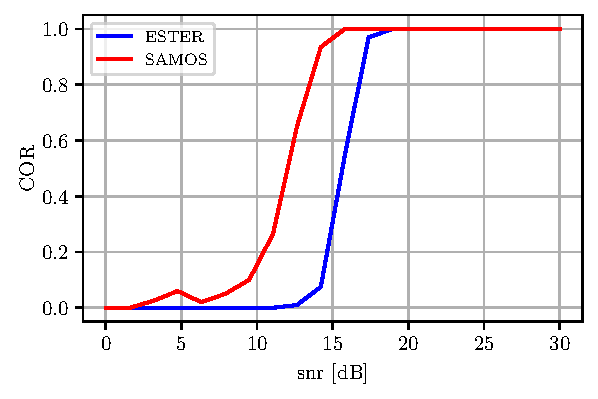
\includegraphics[width = 0.7\textwidth]{Figuras/COR_ESTER_SAMOS_pruebas.pdf}
	\caption{COR para $ESTER$ y SAMOS en función de la SNR.}
	\label{fig:COR_example_SAMOS_ESTER}
\end{figure}

El desempeño de ESTER y SAMOS se puede ver en la figura \ref{fig:COR_example_SAMOS_ESTER}. Se puede observar que cuando $s$ es cercano a $r$ los ángulos $\vartheta_i(s)$, $i=1,\ldots,s$ son pequeños, y $\sin(\vartheta_i(s))$ es muy sensible a pequeñas perturbaciones. Como consecuencia, tanto ESTER como SAMOS presentan un mal desempeño cuando el nivel de ruido es alto. Aunque en SAMOS, el promedio mostrado en \eqref{eq:SamosBoundHy} puede reducir el efecto del ruido, no es completamente efectivo cuando se trabaja con relaciones señal-ruido bajas. Por otro lado, en régimen de alta SNR obtiene un buen desempeño  




\newpage
\section{Apéndice}
\subsection{Algoritmo DBSCAN}

	DBSCAN define grupos como áreas en el espacio de datos donde hay muchos puntos cercanos entre sí. Como entrada recibe dos parámetros 
	\begin{itemize}
		\item $\delta$, determina la distancia máxima entre dos puntos para que uno sea considerado vecino del otro.
		\item $m$, es el número mínimo de puntos dentro de $\delta$ para que un punto sea considerado núcleo.
	\end{itemize}
	
	Luego, el algoritmo distingue entre diferentes tipo de puntos,
	
	\begin{itemize}
		\item Los \textbf{puntos centrales} son aquellos con al menos $m$ puntos es su vecindario de radio $\delta$.
		\item Los \textbf{puntos de borde} son puntos que caen dentro del radio $\delta$ de un punto central pero no tienen suficientes puntos vecinos para considerarlos puntos centrales.
		\item \textbf{Puntos de ruido}, son datos que no son ni puntos centrales ni puntos de borde
	\end{itemize}


DBSCAN comienza con un punto de datos arbitrario e identifica su vecindario (puntos de datos dentro de la distancia $\delta$). Si el vecindario contiene al menos $m$ puntos, se forma un grupo agregando todos los puntos en el vecindario al grupo. El proceso continúa expandiendo el grupo para incluir puntos centrales conectados y sus respectivos vecindarios. El algoritmo continúa visitando los puntos no visitados y comenzará una nueva clase si se encuentra otro punto central. Esta clase también se puede ampliar y así sucesivamente. Finalmente, todos los puntos que no están asignados a una clase son puntos de ruido. El pseudocódigo de DBSCAN se describe en el algoritmo \eqref{Algorithm_DBSCAN}.

\begin{algorithm}
	\caption{Pseudo-código para el algoritmo DBSCAN \cite{ester1996}}
	\begin{algorithmic}[1]
		\State{\textbf{Entradas}: Conjunto de puntos $\setX$; distancia máxima $\delta$; mínima cantidad de puntos para formar un grupo $m$.}
		\State{\textbf{Salidas}: Conjunto de grupos.}
		\Function{DBSCAN}{$\setX$, $\delta$, $m$}
			\State $C \gets 0$ \Comment{Contador de grupos}
			\For{\textbf{cada} punto no visitado $x\in\setX$}
				\State \textbf{Etiquetar} $x$ como ``visitado''	
				\State $Vecinos\gets$ \Call{ConsultaRegion}{$x$,$\delta$}
				\If{$|Vecinos|<m$}
					\State \textbf{marcar} $x$ como punto de ruido
				\Else
					\State $C\gets$ siguiente grupo
					\State \Call{expandirCluster}{$x$, $Vecinos$, $C$, $\delta$, $m$}
				\EndIf
			\EndFor
		\EndFunction
		\Function{expandirCluster}{$x$, Vecinos, $\delta$, $m$}
			\State \textbf{añadir} $x$ al grupo $C$
			\For{\textbf{cada} $p\in Vecinos$}
				\If{$p$ no esta etiquetado como ``visitado''}
					\State \textbf{Etiquetar} $p$ como ``visitado''
					\State $Vecinos' \gets$\Call{ConsultaRegion}{$p$, $\delta$}
					\If{$|Vecinos'|\geq m$}
						\State $Vecinos \gets Vecinos \cup Vecinos'$
					\EndIf
				\EndIf
				\If{$p$ aún no es miembro de ningún Grupo}
					\State \textbf{añadir} $p$ al grupo $C$
				\EndIf
			\EndFor
		\EndFunction
		 \Function{ConsultaRegion}{p, $\delta$}
				\State \textbf{devolver} todos los puntos dentro de una distancia $\delta$ desde el punto $x$
		\EndFunction
	\end{algorithmic}
	\label{Algorithm_DBSCAN}
\end{algorithm} 


 
 